\documentclass[]{ctexbook}
\usepackage{lmodern}
\usepackage{amssymb,amsmath}
\usepackage{ifxetex,ifluatex}
\usepackage{fixltx2e} % provides \textsubscript
\ifnum 0\ifxetex 1\fi\ifluatex 1\fi=0 % if pdftex
  \usepackage[T1]{fontenc}
  \usepackage[utf8]{inputenc}
\else % if luatex or xelatex
  \ifxetex
    \usepackage{xltxtra,xunicode}
  \else
    \usepackage{fontspec}
  \fi
  \defaultfontfeatures{Ligatures=TeX,Scale=MatchLowercase}
\fi
% use upquote if available, for straight quotes in verbatim environments
\IfFileExists{upquote.sty}{\usepackage{upquote}}{}
% use microtype if available
\IfFileExists{microtype.sty}{%
\usepackage{microtype}
\UseMicrotypeSet[protrusion]{basicmath} % disable protrusion for tt fonts
}{}
\usepackage[b5paper,tmargin=2.5cm,bmargin=2.5cm,lmargin=3.5cm,rmargin=2.5cm]{geometry}
\usepackage[unicode=true]{hyperref}
\PassOptionsToPackage{usenames,dvipsnames}{color} % color is loaded by hyperref
\hypersetup{
            pdftitle={rBAS使用文档},
            pdfauthor={王江宇},
            colorlinks=true,
            linkcolor=Maroon,
            citecolor=Blue,
            urlcolor=Blue,
            breaklinks=true}
\urlstyle{same}  % don't use monospace font for urls
\usepackage{natbib}
\bibliographystyle{apalike}
\usepackage{color}
\usepackage{fancyvrb}
\newcommand{\VerbBar}{|}
\newcommand{\VERB}{\Verb[commandchars=\\\{\}]}
\DefineVerbatimEnvironment{Highlighting}{Verbatim}{commandchars=\\\{\}}
% Add ',fontsize=\small' for more characters per line
\usepackage{framed}
\definecolor{shadecolor}{RGB}{248,248,248}
\newenvironment{Shaded}{\begin{snugshade}}{\end{snugshade}}
\newcommand{\KeywordTok}[1]{\textcolor[rgb]{0.13,0.29,0.53}{\textbf{#1}}}
\newcommand{\DataTypeTok}[1]{\textcolor[rgb]{0.13,0.29,0.53}{#1}}
\newcommand{\DecValTok}[1]{\textcolor[rgb]{0.00,0.00,0.81}{#1}}
\newcommand{\BaseNTok}[1]{\textcolor[rgb]{0.00,0.00,0.81}{#1}}
\newcommand{\FloatTok}[1]{\textcolor[rgb]{0.00,0.00,0.81}{#1}}
\newcommand{\ConstantTok}[1]{\textcolor[rgb]{0.00,0.00,0.00}{#1}}
\newcommand{\CharTok}[1]{\textcolor[rgb]{0.31,0.60,0.02}{#1}}
\newcommand{\SpecialCharTok}[1]{\textcolor[rgb]{0.00,0.00,0.00}{#1}}
\newcommand{\StringTok}[1]{\textcolor[rgb]{0.31,0.60,0.02}{#1}}
\newcommand{\VerbatimStringTok}[1]{\textcolor[rgb]{0.31,0.60,0.02}{#1}}
\newcommand{\SpecialStringTok}[1]{\textcolor[rgb]{0.31,0.60,0.02}{#1}}
\newcommand{\ImportTok}[1]{#1}
\newcommand{\CommentTok}[1]{\textcolor[rgb]{0.56,0.35,0.01}{\textit{#1}}}
\newcommand{\DocumentationTok}[1]{\textcolor[rgb]{0.56,0.35,0.01}{\textbf{\textit{#1}}}}
\newcommand{\AnnotationTok}[1]{\textcolor[rgb]{0.56,0.35,0.01}{\textbf{\textit{#1}}}}
\newcommand{\CommentVarTok}[1]{\textcolor[rgb]{0.56,0.35,0.01}{\textbf{\textit{#1}}}}
\newcommand{\OtherTok}[1]{\textcolor[rgb]{0.56,0.35,0.01}{#1}}
\newcommand{\FunctionTok}[1]{\textcolor[rgb]{0.00,0.00,0.00}{#1}}
\newcommand{\VariableTok}[1]{\textcolor[rgb]{0.00,0.00,0.00}{#1}}
\newcommand{\ControlFlowTok}[1]{\textcolor[rgb]{0.13,0.29,0.53}{\textbf{#1}}}
\newcommand{\OperatorTok}[1]{\textcolor[rgb]{0.81,0.36,0.00}{\textbf{#1}}}
\newcommand{\BuiltInTok}[1]{#1}
\newcommand{\ExtensionTok}[1]{#1}
\newcommand{\PreprocessorTok}[1]{\textcolor[rgb]{0.56,0.35,0.01}{\textit{#1}}}
\newcommand{\AttributeTok}[1]{\textcolor[rgb]{0.77,0.63,0.00}{#1}}
\newcommand{\RegionMarkerTok}[1]{#1}
\newcommand{\InformationTok}[1]{\textcolor[rgb]{0.56,0.35,0.01}{\textbf{\textit{#1}}}}
\newcommand{\WarningTok}[1]{\textcolor[rgb]{0.56,0.35,0.01}{\textbf{\textit{#1}}}}
\newcommand{\AlertTok}[1]{\textcolor[rgb]{0.94,0.16,0.16}{#1}}
\newcommand{\ErrorTok}[1]{\textcolor[rgb]{0.64,0.00,0.00}{\textbf{#1}}}
\newcommand{\NormalTok}[1]{#1}
\usepackage{longtable,booktabs}
% Fix footnotes in tables (requires footnote package)
\IfFileExists{footnote.sty}{\usepackage{footnote}\makesavenoteenv{long table}}{}
\usepackage[normalem]{ulem}
% avoid problems with \sout in headers with hyperref:
\pdfstringdefDisableCommands{\renewcommand{\sout}{}}
\IfFileExists{parskip.sty}{%
\usepackage{parskip}
}{% else
\setlength{\parindent}{0pt}
\setlength{\parskip}{6pt plus 2pt minus 1pt}
}
\setlength{\emergencystretch}{3em}  % prevent overfull lines
\providecommand{\tightlist}{%
  \setlength{\itemsep}{0pt}\setlength{\parskip}{0pt}}
\setcounter{secnumdepth}{5}
% Redefines (sub)paragraphs to behave more like sections
\ifx\paragraph\undefined\else
\let\oldparagraph\paragraph
\renewcommand{\paragraph}[1]{\oldparagraph{#1}\mbox{}}
\fi
\ifx\subparagraph\undefined\else
\let\oldsubparagraph\subparagraph
\renewcommand{\subparagraph}[1]{\oldsubparagraph{#1}\mbox{}}
\fi

% set default figure placement to htbp
\makeatletter
\def\fps@figure{htbp}
\makeatother

\usepackage{booktabs}
\usepackage{longtable}

\usepackage{framed,color}
\definecolor{shadecolor}{RGB}{248,248,248}

\renewcommand{\textfraction}{0.05}
\renewcommand{\topfraction}{0.8}
\renewcommand{\bottomfraction}{0.8}
\renewcommand{\floatpagefraction}{0.75}

\let\oldhref\href
\renewcommand{\href}[2]{#2\footnote{\url{#1}}}

\makeatletter
\newenvironment{kframe}{%
\medskip{}
\setlength{\fboxsep}{.8em}
 \def\at@end@of@kframe{}%
 \ifinner\ifhmode%
  \def\at@end@of@kframe{\end{minipage}}%
  \begin{minipage}{\columnwidth}%
 \fi\fi%
 \def\FrameCommand##1{\hskip\@totalleftmargin \hskip-\fboxsep
 \colorbox{shadecolor}{##1}\hskip-\fboxsep
     % There is no \\@totalrightmargin, so:
     \hskip-\linewidth \hskip-\@totalleftmargin \hskip\columnwidth}%
 \MakeFramed {\advance\hsize-\width
   \@totalleftmargin\z@ \linewidth\hsize
   \@setminipage}}%
 {\par\unskip\endMakeFramed%
 \at@end@of@kframe}
\makeatother

\makeatletter
\@ifundefined{Shaded}{
}{\renewenvironment{Shaded}{\begin{kframe}}{\end{kframe}}}
\@ifpackageloaded{fanyverb}{%
  % https://github.com/CTeX-org/ctex-kit/issues/331
  \RecustomVerbatimEnvironment{Highlighting}{Verbatim}{commandchars=\\\{\},formatcom=\xeCJKVerbAddon}%
}{}
\makeatother

\usepackage{makeidx}
\makeindex

\urlstyle{tt}

\usepackage{amsthm}
\makeatletter
\def\thm@space@setup{%
  \thm@preskip=8pt plus 2pt minus 4pt
  \thm@postskip=\thm@preskip
}

\makeatother

\makeatletter
\def\CTEX@section@format{\Large\bfseries\flushleft}
\makeatother

\frontmatter

\title{rBAS使用文档}
\author{王江宇}
\date{2019-02-02}

\let\BeginKnitrBlock\begin \let\EndKnitrBlock\end
\begin{document}
\maketitle

{
\setcounter{tocdepth}{2}
\tableofcontents
}
\listoftables
\listoffigures
\mainmatter

\chapter*{前言}


\section*{手册内容概述}


本手册是为了大家更好地使用\textbf{rBAS}\index{rBAS}
\citep{R-rBAS}包而撰写,内容如下:

\begin{itemize}
\item
  第 \ref{install}
  章介绍了如何安装\texttt{R}语言的环境,来使用\texttt{rBAS}包。不用担心,\texttt{R}的语法很简单,各种功能是按照自身的需要安装各种\texttt{packages},所以比\texttt{matlab}体积更小,入门时间成本也较低。\textbf{哪怕你无意于\texttt{R}的学习,也可以看看本手册的原理篇(第
  \ref{algorithm} 章),应用篇(第\ref{examples}章)以及后续的更新计划(第
  \ref{updates}
  章),来了解算法的原理,出现了哪些变种,以及有着什么样的工程应用}。
\item
  第 \ref{algorithm}
  章介绍了\textbf{BAS算法}以及在其基础上出现的各种\textbf{改进算法}的\textbf{原理},当然,随着算法的不断改进和发展,这个文档还需要随之不断更新。
\item
  第 \ref{mixedalgorithm}
  章中介绍了BAS与其他算法结合的算法。目前收录的有,王糖糖同学提供的BSO,即BAS和PSO的结合。\texttt{rBAS}包也提供了这些算法的实现与调用。
\item
  第 \ref{rBAS}
  章讲述了如何在\texttt{R}中使用\texttt{rBAS}包\textbf{调用收录的算法的对应函数},以及一些简单的\textbf{案例}(大部分是\texttt{BAS}相关文献中的算例和\texttt{benchmark\ functions})。每一句出现的代码我都会尽我所能去注释,让大家了解每一步的意义,以及\texttt{R}的简单易用。我也希望,自己的语言能尽力通俗,对于其他工具的使用者来说。
\item
  第 \ref{interface} 章介绍了\texttt{rBAS}中的用户界面的调用,以及运行。
\item
  第 \ref{examples}
  章主要介绍的是BAS及变体算法\textbf{在多杆机构优化中的应用},由群友莫小娟同学提供。
\item
  第 \ref{examples2}
  章主要介绍的是BAS及变体算法\textbf{在龙门起重机控制优化中的应用},由群友李晓晓同学提供。
\item
  第 \ref{python}
  章主要介绍吴会欢同学提供的python接口,目前有基本的BAS,以及三个测试函数,后续会持续更新。
\item
  第 \ref{matlabr} 章中主要介绍了两种方法供matlab用户来使用rBAS
  package。当然,未来可能会出现matlab中R的接口,或者是BAS
  toolbox,到时候此章无用。如果你发现了\textbf{更便捷的方法},来实现两者的通讯,还请\href{https://github.com/jywang2016/rBAS_documents/issues}{提出建议}。
\item
  第 \ref{paper} 章用于收录基于BAS及相关算法的工具箱,软件或者文献等等。
\item
  第 \ref{updates}
  章讲述了\texttt{rBAS}包的\textbf{开发和使用手册更新的计划}。因为算法总是会不断地推陈出新,所以\texttt{rBAS}包也必须和目前的研究保持一致。如果你有好的想法,可以看此章的内容,然后把自己的建议传达给我们。
\end{itemize}

\begin{quote}
好了,冗长的章节介绍完毕。大家可以开始浏览正文了。
\end{quote}

由于后续的案例中,会带有大量的动态图片。为了方便大家的浏览,强烈推荐在网页上阅读本手册,\url{https://jywang2016.github.io/rBAS_documents/}
。此外,由于个人能力与时间有限,希望大家看到相关的BAS文章或者工作后,可以在
\url{https://github.com/jywang2016/rBAS_documents/issues}
上\textbf{写明文章的信息,应用的领域以及采用的是哪种BAS算法},以此来帮助我的整理。十分感谢大家的帮助!

\section*{夹带私货}


如果你对这本手册本身的撰写环境感兴趣的话,那我可能还要啰嗦两句。

\emph{第一句}:照搬 \href{http://yihui.name/}{Yihui}
的一句话:我用了两个 R 包编译这本书,分别是 \textbf{knitr}\index{knitr}
\citep{xie2015} 和 \textbf{bookdown}\index{bookdown}
\citep{R-bookdown}。

\emph{第二句}:感谢
Yihui。嗯\ldots{},因为这个男人,R用户的读书笔记,文章,学位论文,个人网站等等都可以在R里面撰写或者开发。不得不感慨他的天才和对需求的把握。

\section*{致谢}


感谢提倡者\texttt{李帅}老师,以及\texttt{姜向远}博士。他们是\texttt{BAS}的提出者,也在算法原理与改进上,给了我这个做暖通的门外汉以启发。

此外,还感谢\texttt{李晓晓},\texttt{王甜甜},\texttt{莫小娟},\texttt{阮月}同学贡献自己的算法代码和应用案例,他(她)们改进了算法,并且让其应用部分变得更加丰富。

感谢\texttt{吴会欢}同学提供了\texttt{python}的接口,虽然目前只有基本的BAS,但后续会更加完善。

当然,还得感谢Yihui的\texttt{bookdown}。

老实讲,2018/07,也就是一个月以前,我刚开始用\texttt{R}编写这个算法,然后用在自己的建筑系统辨识研究中,没想到\(\dots\)
所以,这个手册是比较仓促的产物,再加之自身关于优化算法理论水平较低,如果大家发现了本手册的各种问题,欢迎在QQ群(437958608)内留言,或者是在\texttt{rBAS}的
github上提出 \href{https://github.com/jywang2016/rBAS/issues}{issues}。

总之,谢谢上述老师及同学,也谢谢未来给我提供问题或建议的同学,你们的帮助,让手册更加完善。

最后的最后,希望大家尽量用
\url{https://jywang2016.github.io/rBAS_documents/}
来访问本手册,PDF不支持案例中的动态图片展示。

\BeginKnitrBlock{flushright}
王江宇\\
2018/08/18\\
华中科技大学
\EndKnitrBlock{flushright}

\chapter*{作者简介}\label{author}


\begin{itemize}
\tightlist
\item
  包作者

  \begin{itemize}
  \tightlist
  \item
    王江宇:
    \texttt{BSAS}算法,创建维护\texttt{rBAS}包。\href{https://github.com/jywang2016/rBAS}{Github}
  \item
    李帅:
    提出\texttt{BAS}以及\texttt{BAS-WPT}算法。\href{http://www4.comp.polyu.edu.hk/~cssli/}{个人主页}
    \&
    \href{http://scholar.google.com/citations?hl=zh-CN\&user=H8UOWqoAAAAJ}{谷歌学术}
  \item
    姜向远: 提出\texttt{BAS}以及\texttt{BAS-WPT}算法。
  \end{itemize}
\item
  贡献者

  \begin{itemize}
  \tightlist
  \item
    李晓晓: 二阶\texttt{BAS}
  \item
    王甜甜: 天牛群体优化算法\texttt{BSO}
  \item
    阮月: \texttt{Binary-BAS}
  \item
    莫小娟: 多杆机构优化问题
  \end{itemize}
\end{itemize}

\chapter{R以及rBAS安装}\label{install}

\texttt{R}以及其集成开发环境(IDE)\texttt{Rstudio}加起来都不到200M,所以大家放心下载安装,不会是需要10+G的庞然大物。当然,\texttt{matlab}也是很好的科学计算软件,这里仅仅是说明安装的大小。

总体来说,R的安装十分简单,类似于把大象装进冰箱只需要三步。

\section{R安装}\label{Rinstall}

\texttt{Step1}: 进入R的网站 \url{https://www.r-project.org/}
,然后点击左上角\texttt{Download}底下的\texttt{CRAN}。

\texttt{Step2}:
选择并点击\texttt{China}底下的镜像网址,方便下载。然后点击\texttt{Download\ R\ for\ windows},出现的界面右上角有\texttt{install\ R\ for\ the\ first\ time},点击即可下载。

\texttt{Step3}: 安装,不需要各种复杂的配置,按照给定提示操作即可。

但是,打开R,你会发现是如图\ref{fig:rface}这样过于\texttt{简洁}的界面。

\begin{figure}

{\centering 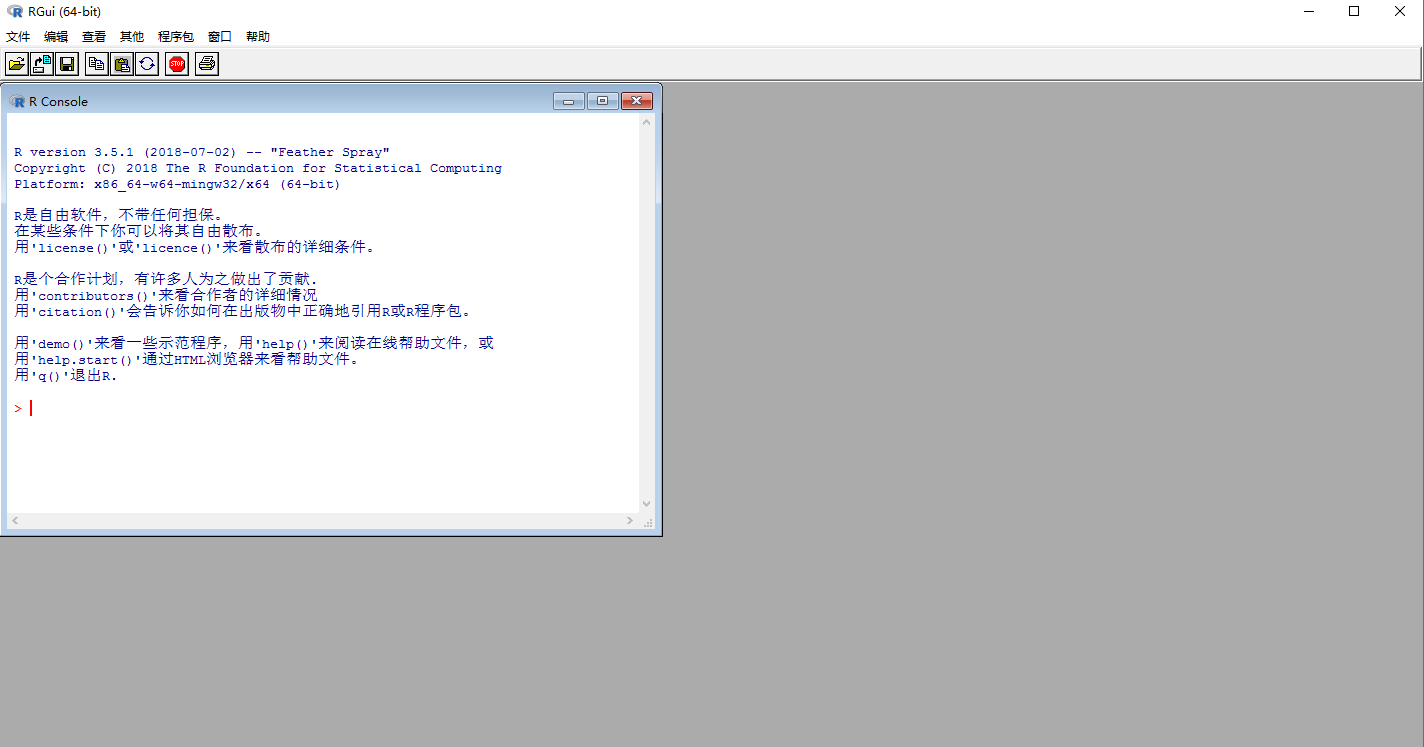
\includegraphics[width=0.8\linewidth]{img/R} 

}

\caption{R界面}\label{fig:rface}
\end{figure}

这并不符合新手的操作和开发习惯。因此,你可能需要一个集成开发环境,最好是有函数、变量的提示,方便浏览代码和结果等等优势的软件。那么,我想你说的应该是
\texttt{Rstudio}。

\section{Rstudio安装}\label{Rstudioinstall}

\texttt{Step1}: 进入下载页面
\url{https://www.rstudio.com/products/rstudio/download/} 。

\texttt{Step2}: 选择\texttt{free}版本的下载。

\texttt{Step3}: 安装,无需配置特别的环境变量等。

那么,打开\texttt{Rstudio}后,会看到如图\ref{fig:rstudioface}这样的界面。

\begin{figure}

{\centering 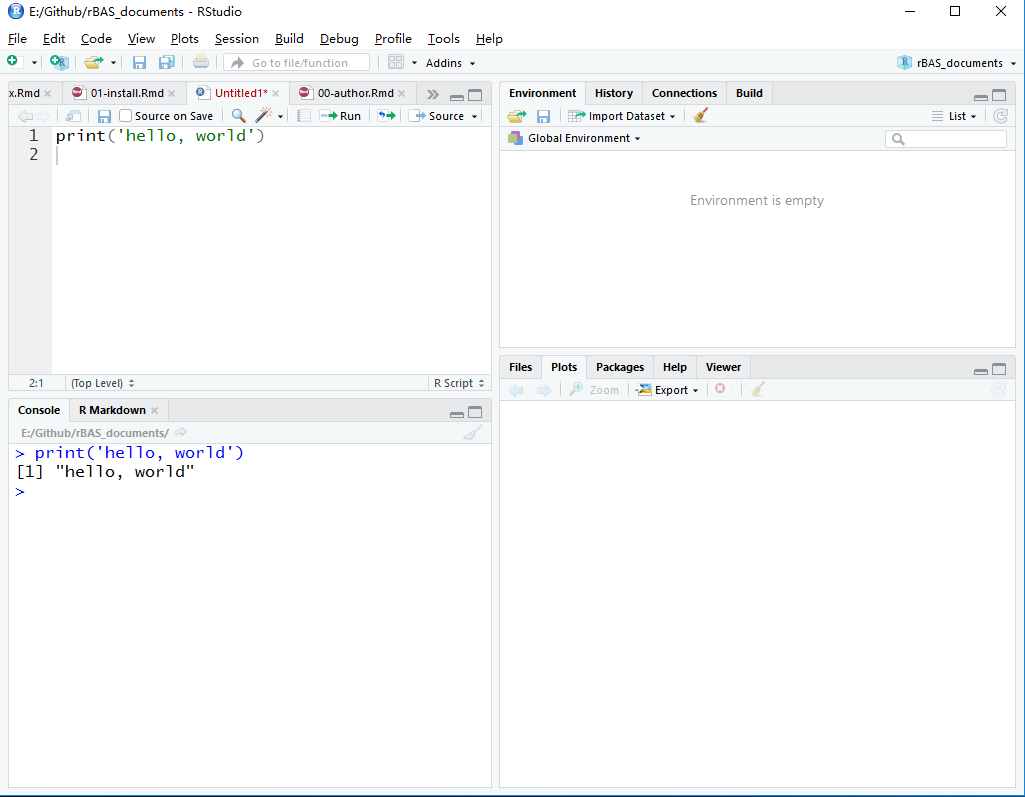
\includegraphics[width=0.8\linewidth]{img/Rstudio} 

}

\caption{Rstudio界面}\label{fig:rstudioface}
\end{figure}

左上角是撰写代码脚本的区域,左下角是结果输出的窗口。右下角的\texttt{files}可以查看工作路径下的文件,和\texttt{matlab}左侧的栏目是类似的;\texttt{plots}用于查看使用代码绘制的图像,\texttt{packages}可以用于安装\texttt{CRAN}上发布,或者是本地的\texttt{packages},也就类似\texttt{matlab}的\texttt{toolbox};\texttt{help}则是用来显示各个函数的帮助文档;\texttt{Viewer}则是用来预览\texttt{R}生成的交互图像(比如\texttt{plotly}绘制的图),生成的网页(比如我现在正在使用\texttt{bookdown}包来写本手册,那就可以预览生成的\texttt{gitbook}电子书的内容)等等。右上角的\texttt{Environment}显示被加载进来的函数,变量等信息,和\texttt{matlab}的\texttt{workspace}是类似的。
剩下的和本手册无关,可以在后面的开发中慢慢了解。

\section{rBAS安装}\label{rBASinstall}

在\texttt{Rstudio}的\texttt{Console}框内输入:

\begin{Shaded}
\begin{Highlighting}[]
\KeywordTok{install.packages}\NormalTok{(}\StringTok{'devtools'}\NormalTok{)}
\end{Highlighting}
\end{Shaded}

因为目前\texttt{rBAS}包还不在\texttt{CRAN}内,所以需要通过\texttt{devtools}包,来从\texttt{github}上安装。所以我们先在本地安装\texttt{devtools}包。如果觉得代码敲的累,那么有个更直观的方式,如图\ref{fig:devtools}:

\begin{figure}

{\centering 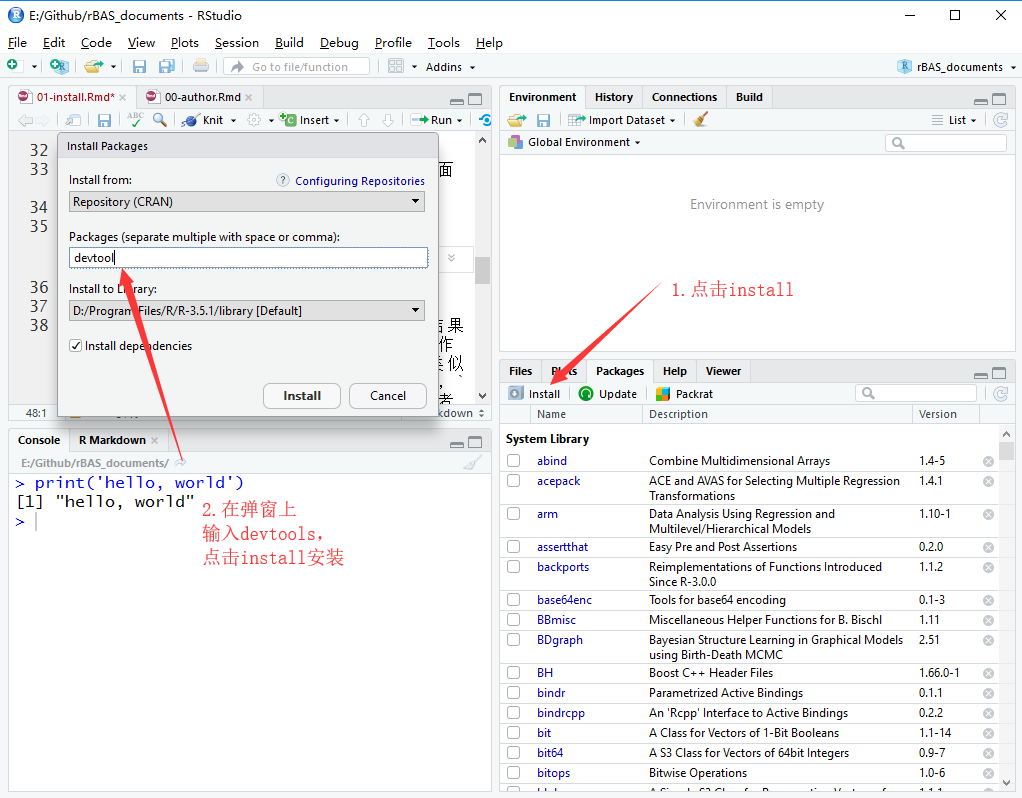
\includegraphics[width=0.8\linewidth]{img/rBAS} 

}

\caption{devtools手动安装示意图}\label{fig:devtools}
\end{figure}

最后,有了\texttt{devtools}包,我们可以从\texttt{github}上安装\texttt{rBAS}包了。

\begin{Shaded}
\begin{Highlighting}[]
\CommentTok{#不加载devtools,只调用其中的函数}
\NormalTok{devtools}\OperatorTok{::}\KeywordTok{install_github}\NormalTok{(}\StringTok{"jywang2016/rBAS"}\NormalTok{)}
\end{Highlighting}
\end{Shaded}

接下来,我们可以使用\texttt{rBAS}的函数了。

\chapter{算法原理}\label{algorithm}

本章讲述目前\texttt{rBAS}集成的三种算法,即\texttt{BAS},\texttt{BSAS},\texttt{BSAS-WPT}的原理。如有错漏,还请指出。此外,本章所述的算法,在原始的\texttt{BAS}基础上,并没有过多地改变根本上的东西。第\ref{mixedalgorithm}章的算法,则是\texttt{BAS}和其他一些算法的结合,又或者,有更多根本性改动。如王糖糖同学提出的\texttt{BSO},很典型地\texttt{BAS}和\texttt{PSO}的结合,则不在此章节。

\section{BAS}\label{bas}

关于\texttt{BAS},主要的参考资料为\texttt{姜向远}博士和\texttt{李帅}老师在\texttt{arXiv}上的论文,\href{https://arxiv.org/abs/1710.10724}{BAS:
beetle antennae search algorithm for optimization
problems}。而我是在知乎上看到一篇\href{https://zhuanlan.zhihu.com/p/30742461}{文章}后,才开始复现\texttt{BAS}算法。

\subsection{算法流程}\label{BASflow}

1.随机生成方向向量,标准化

\begin{equation}
\overrightarrow{\mathbf{b}}=\frac{\text{rnd}(n,1)}{\|\text{rnd}(n,1)\|}
\label{eq:dir}
\end{equation}

其中,\(n\)是待优化参数的维度。

2.计算左右须的坐标

\begin{equation}
\begin{split}
\mathbf{x}_r&=\mathbf{x}^t+d^t\overrightarrow{\mathbf{b}} \\
\mathbf{x}_l&=\mathbf{x}^t-d^t\overrightarrow{\mathbf{b}}
\end{split}
\label{eq:xlxr}
\end{equation}

其中,\(\mathbf{x}^t\)为\(t\)时刻天牛的位置,\(d^t\)则是\(t\)时刻,质心到须的距离。

3.根据两须对应函数值,决定天牛下一时刻移动位置

\begin{equation}
\mathbf{x}^t=\mathbf{x}^{t-1}+\delta^t\overrightarrow{\mathbf{b}}\text{sign}(f(\mathbf{x}_r)-f(\mathbf{x}_l))
\label{eq:xupdate}
\end{equation}

其中,\(\delta^t\)为t时刻的步长,\(f\)为待优化目标函数。

4.步长与搜索距离更新

\begin{align}
d^t&= \eta_d d^{t-1}+d_0 \label{eq:dupdate}\\
\delta^t&=\eta_{\delta} \delta^{t-1} \label{eq:deltaupdate}
\end{align}

其中,\(d_0\)是人为设定的距离的常数,\(\eta_d\)与\(\eta_\delta\)分别是搜索距离和步长的更新衰减系数。

为了避免参数过多,姜向远博士在\texttt{BAS-WPT}算法中是按照式\eqref{eq:WPTupdate}来更新搜索距离和步长的。其中,\(c_2\)是人为设定的常数。

\begin{equation}
\begin{split}
\delta^t&=\eta_{\delta} \delta^{t-1}\\
d^t &= \frac{\delta^t}{c_2}\\
\end{split}
\label{eq:WPTupdate} 
\end{equation}

\subsection{不足与改进}\label{BASimprove}

在对\texttt{BAS}算法的复现与案例应用中,我个人认为,其可能存在如下的缺点。

\begin{itemize}
\tightlist
\item
  步长更新策略(反馈)

  \begin{itemize}
  \tightlist
  \item
    缺点:无论每一步得到的结果是否变得更优,步长总会衰减;
  \item
    改进:带有反馈的步长更新,在无法找到更优的位置时,才进行步长的更新;
  \item
    关键:反馈
  \end{itemize}
\item
  初始步长选取(参数标准化)

  \begin{itemize}
  \tightlist
  \item
    缺点:对于多参数且量纲相差较大的问题,步长 \(\delta\)
    的初始值并不好选取;
  \item
    改进:标准化参数后,再进行调节,这也是\texttt{BAS-WPT}的技巧所在;
  \item
    关键:标准化
  \end{itemize}
\item
  群体寻优

  \begin{itemize}
  \tightlist
  \item
    缺点:1只天牛在随机方向上搜索更优的位置,容易迷失;
  \item
    改进:多只天牛寻优,设定的回合内无法找到更优位置,再考虑步长更新;
  \item
    关键:群体智能
  \end{itemize}
\item
  约束处理能力不足

  \begin{itemize}
  \tightlist
  \item
    缺点:在约束边界上优化目标突变问题的处理上表现不佳
  \item
    改进:二阶\texttt{BAS}
  \item
    关键:\texttt{暂时没有能力归纳},有待学习二阶\texttt{BAS}
  \end{itemize}
\end{itemize}

\section{BSAS}\label{bsas}

在\ref{BASimprove}节中提及,\texttt{BAS}可能在\textbf{步长更新}和\textbf{群体寻优}两个方面的策略上有一定的不足。因此,我比较莽撞地改出一个粗糙的算法,那就是所谓的\texttt{BSAS},即\texttt{beetle\ swarm\ antennae\ search}。在\href{https://arxiv.org/abs/1807.10470}{\texttt{BSAS:\ Beetle\ Swarm\ Antennae\ Search\ Algorithm\ for\ Optimization\ Problems}}中,我给出了更为详细的材料。至于具体和\texttt{王甜甜}同学的\texttt{BSO},即\texttt{beetle\ swarm\ optimization}有何不同,我需要进一步研究她的论文材料。

\subsection{与BAS不同之处}\label{BSASflow}

此部分没有公式,因为和\texttt{BAS}算法核心公式思路是一致的。而图\ref{fig:basflow}与图\ref{fig:bsasflow}描述了一种假设的寻优场景,能比较清晰地体现\texttt{BSAS}与\texttt{BAS}之间的不同。

\begin{figure}

{\centering 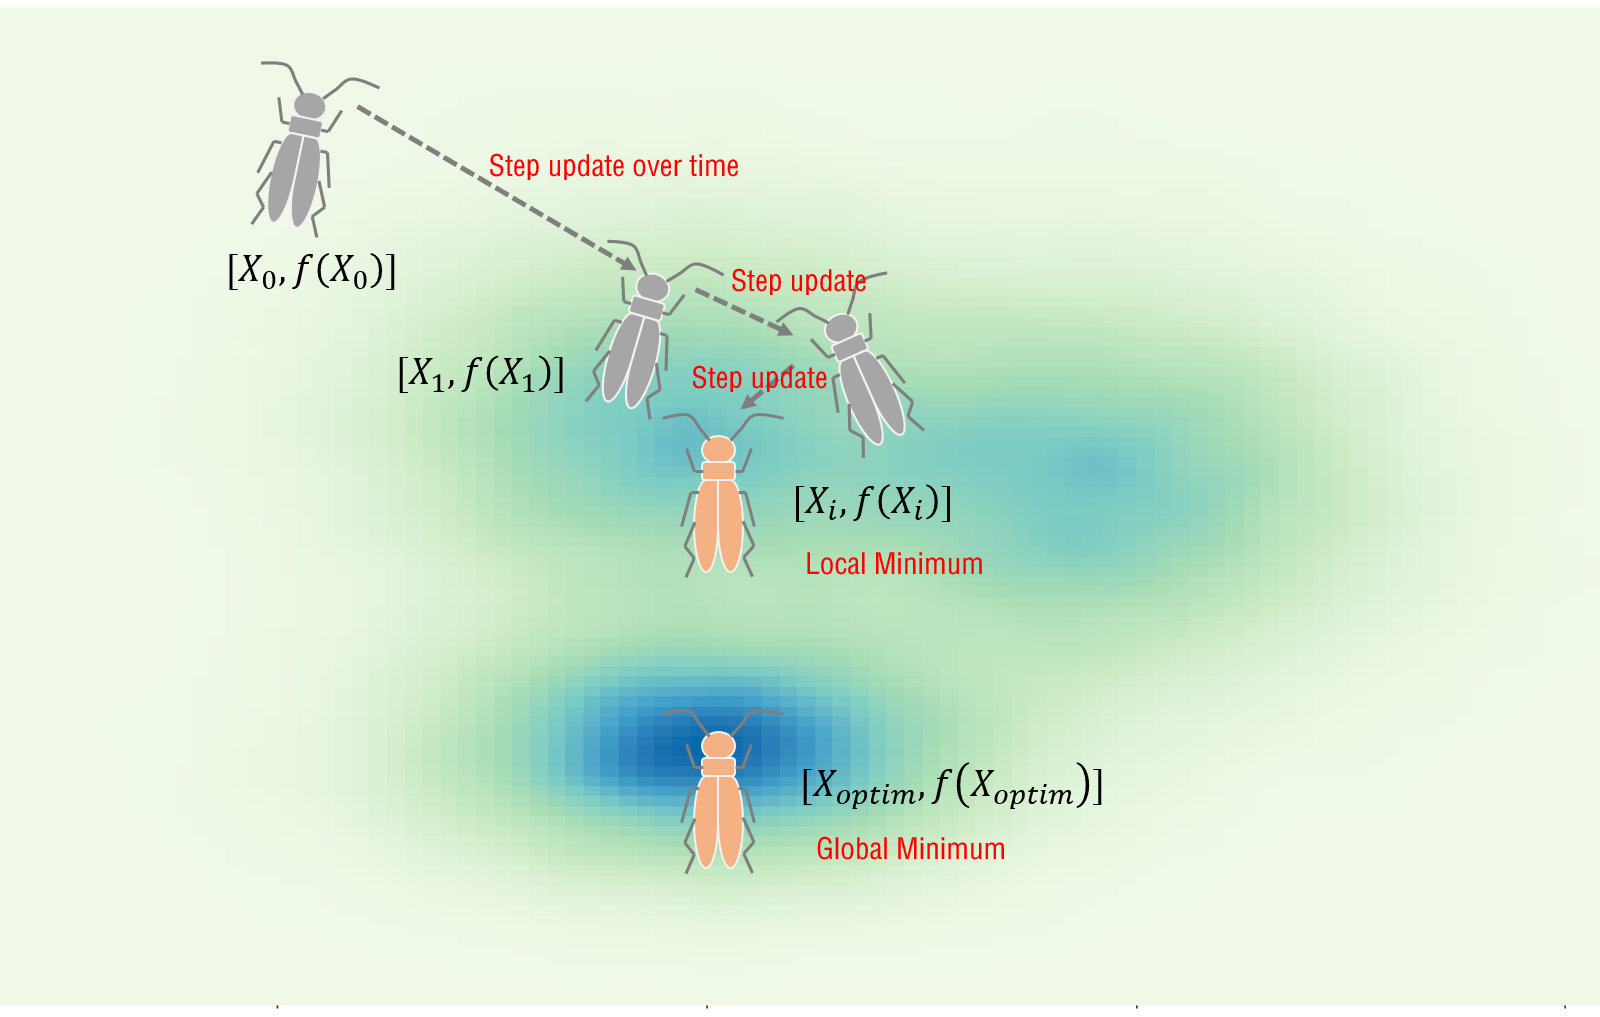
\includegraphics[width=0.8\linewidth]{img/BAS} 

}

\caption{BAS寻优过程示意}\label{fig:basflow}
\end{figure}

\begin{figure}

{\centering 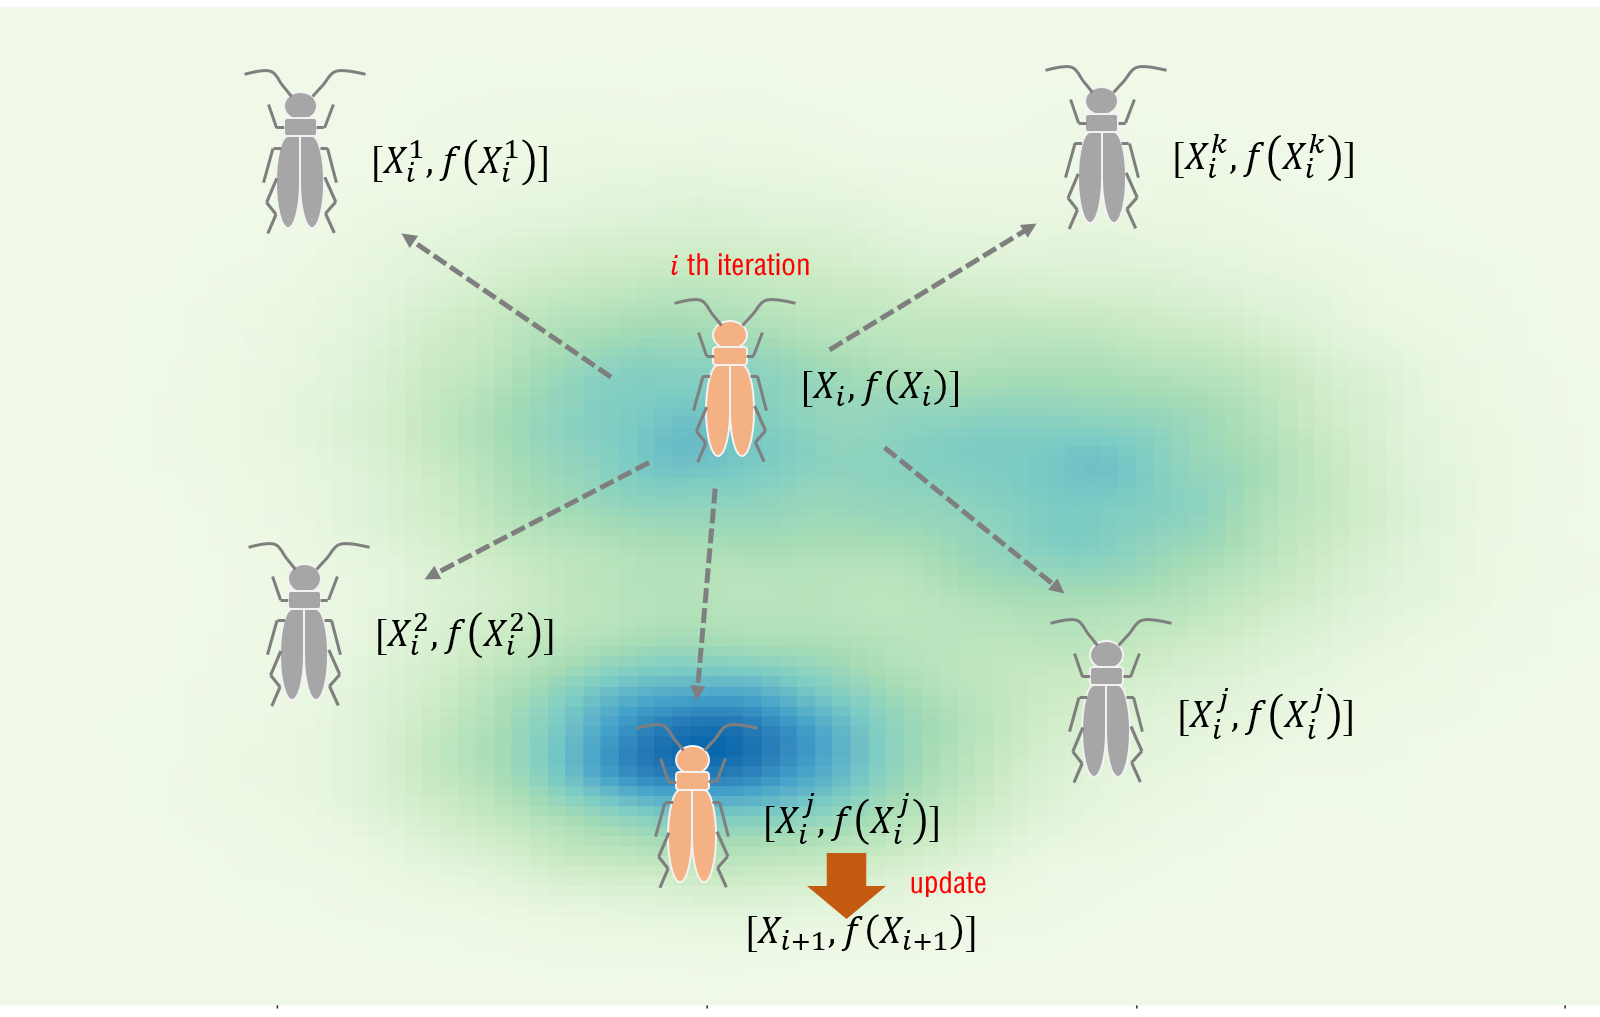
\includegraphics[width=0.8\linewidth]{img/BSAS} 

}

\caption{BSAS寻优过程示意}\label{fig:bsasflow}
\end{figure}

假定,天牛要找到图中\textbf{最蓝的点}。图\ref{fig:basflow}
中,天牛的起点在距离最优点较远处。由于位置更新只与时间有关,也就是每一步,天牛的步长都会缩减(为了可视化效果,天牛的大小我并没有缩放)。如果初始位置距离最优点较远,那在给定的步长缩减情况下,天牛只能在一个\textbf{局部最优点}处收敛。而图\ref{fig:bsasflow}中,每回合天牛会派出\(k\)只天牛在外试探,如果有更优的点,那么更新天牛位置。这样天牛可以更好地到达\textbf{全局最优点}。

\subsection{不足与改进}\label{BSASimprove}

虽然解决了步长更新和群体寻优的策略问题,但是还有两点并未解决。

\begin{itemize}
\tightlist
\item
  初始步长选取(参数标准化)

  \begin{itemize}
  \tightlist
  \item
    缺点:对于多参数且量纲相差较大的问题,步长 \(\delta\)
    的初始值并不好选取;
  \item
    改进:标准化参数后,再进行调节,这也是\texttt{BAS-WPT}的技巧所在;
  \end{itemize}
\item
  约束处理能力不足

  \begin{itemize}
  \tightlist
  \item
    缺点:在约束边界上优化目标突变问题的处理上表现不佳
  \item
    改进:二阶\texttt{BAS}
  \end{itemize}
\end{itemize}

好的是,在\texttt{rBAS\ 0.1.5}中,我们吸收了\texttt{BAS-WPT}中\textbf{参数标准化}的想法,加入了\texttt{BSAS-WPT}算法,来解决步长调参的问题,并取得了一定的改进效果。

\section{BAS-WPT}\label{bas-wpt}

相比于\ref{BASflow}节中描绘的\texttt{BAS},
\href{https://arxiv.org/abs/1711.02395}{Beetle Antennae Search without
Parameter Tuning (BAS-WPT) for Multi-objective
Optimization}一文给出了改进后的\texttt{BAS}是如何处理\textbf{步长调节}和\textbf{约束问题抽象}的。

\subsection{与BAS不同之处}\label{BASWPTflow}

\texttt{BAS-WPT}的小尾巴\texttt{without\ parameter\ tunning}已经说明了两者之间的区别,即\texttt{BAS-WPT}是不需要进行参数调节的。当然,按照我现在的理解,是\texttt{BAS-WPT}一方面简化了\textbf{每回合搜索距离}(质心到须的距离)的\textbf{更新},不需要再\textbf{额外设定与调节}诸如\(d_0\),\(\eta_d\)等参数,用户只需要按照式\eqref{eq:WPTupdate}来设置\(c_2\)便可;另一方面,参数标准化,让\textbf{存在量级差异}的参数之间不必再像\texttt{BAS}一样,共享一个你不知道该怎么设定的步长\(\delta^t\)(步长过大,小的参数可能经常处于在边界的状态;步长过小,大的参数可能搜索范围达不到)。

那么上述两方面的优势归纳起来是什么呢,那就是你可以设置一个在 \(1\) 附近
\(\delta\) ,然后设定一个衰减率
\(\eta_{\delta}\),以及步长与搜索距离之比
\(c_2\),那么你的天牛就不会出太大的岔子,并且方便调整调节。也就是说,\texttt{WPT}不是让你不用调参,而是减轻了调参的负担。

\begin{quote}
``不必就纠结归一化处理,之所以这么处理,仅仅是为了调参方便''

\begin{flushright}--- 姜向远\end{flushright}
\end{quote}

果然,偷懒催生了这一技巧的诞生。不过,我还得再次啰嗦一句标准化的好(是不是我没有接触这个领域,所以喜欢大惊小怪\ldots{}\ldots{})。我们在之后,压力容器约束问题(\textbf{混合整型规划})中,可以看到,待优化参数存在量级差异时,标准化技巧下的步长会比原始的\texttt{BAS}步长设定要更加合理。

\subsection{约束问题抽象形式}\label{constrform}

此外,\texttt{BAS-WPT}还为\texttt{BAS}引入了约束问题处理的手段。不过,这和我做模型预测控制时候看到的抽象方式是相同的。我觉得\texttt{BAS}的用户们应该都早已了解,此处就照本宣科。

\subsubsection{约束问题一般形式}

\begin{equation}
\begin{split}
& \frac{\text{Minimize}}{\text{Maximize}} f(\mathbf{x}) \\
s.t.  & g_j(\mathbf{x})\leq 0, j=1, \cdots, K \\
& x^\text{max}_i \leq x_i \leq x^\text{min}_i, i=1, \cdots N
\end{split}
\label{eq:ConProb}
\end{equation}

\(g_j(\mathbf{x})\leq 0\) 和
\(x^\text{max}_i \leq x_i \leq x^\text{min}_i\)
表示了参数本身的范围和更为精细具体的不等式约束控制。在\texttt{rBAS}包中,我们会有很\textbf{直观和简便}的方式,来设置这些约束。

\subsubsection{惩罚函数}

\begin{equation}
F(\mathbf{x})=f(\mathbf{x})+\lambda\sum_{j=1}^{K}h_j(\mathbf{x})g_j(\mathbf{x})
\label{eq:penalty}
\end{equation}

\begin{equation}
h_j(\mathbf{x}) = \begin{cases} 
1, & g_j(\mathbf{x})>0 \\ 
0, & g_j(\mathbf{x})\leq0
\end{cases}
\label{eq:violation}
\end{equation}

其中,式\eqref{eq:penalty}中的\(\lambda\)表示约束违背的惩罚因子,选取尽量大的正数。而后的\(h_j(\mathbf{x})\)为\texttt{Heaviside}函数,即不等式约束满足时,该函数为0,反之为1。

\subsection{不足与改进}\label{BSASimprove2}

\begin{itemize}
\tightlist
\item
  约束处理能力不足

  \begin{itemize}
  \tightlist
  \item
    缺点:在约束边界上优化目标突变问题的处理上表现不佳
  \item
    改进:二阶\texttt{BAS}
  \end{itemize}
\end{itemize}

此处的不足,还需要考虑步长反馈和群体搜索的问题。不过,既然\texttt{BSAS}把姜博的\texttt{WPT}给窃来了,摇身变为了\texttt{BSAS-WPT},那就不说上述两个问题了。等他日有闲,再去整合\texttt{李晓晓}同学的二阶\texttt{BAS}。

\section{BAS with momentum(second-order BAS)}\label{BAS2}

带动量的BAS,唔\ldots{}\ldots{}这名字听着有点长。顾名思义,是利用了惯性项(即,前一时刻的状态),来使得算法不陷入局部最优。不得不说,李晓晓同学对算法的改进既保留了BAS本身的简洁,又增大了BAS对局部最优处理的能力。

在打算复现BSO(BAS和PSO的诚意结合)算法之前,我就看过了李晓晓同学提供给我的二阶BAS代码。相比于BSO,进行了大量的细节上的BAS和PSO融合,二阶BAS只对天牛位置更新的等式(即式\eqref{eq:xupdate})做了大的改动。因此,我觉得这还是更为类似BAS的,大家接受起来应该也更为容易。

\subsection{算法原理}

在\ref{BASflow}节的基础上,改动了一大一小两处地方。大的是,天牛位置更新。小的改动是,步长增加了一个最小分辨率,也就是存在了最小值,不会无限制地缩减。

在位置更新上,参考式\eqref{eq:bas2vupdate}至式\eqref{eq:bas2xupdate}。

\begin{equation}
\mathbf{v}^{t+1} = w_0\mathbf{v}^t - w_1\overrightarrow{b}(f(\mathbf{x}_l^t)-f(\mathbf{x}_r^t))
\label{eq:bas2vupdate}
\end{equation}

\begin{equation}
\mathbf{v}^{t+1} = \begin{cases} 
V_{max},&\mathbf{v}^{t+1} > V_{max} \\ 
\mathbf{v}^{t+1},  &\mathbf{v}^{t+1} \in [V_{max},V_{max}] \\
-V_{max},&\mathbf{v}^{t+1} <- V_{max}
\end{cases}
\label{eq:bas2vbound}
\end{equation}

\begin{equation}
\mathbf{x}^{t+1} = \mathbf{x}^t+\mathbf{v}^{t+1}
\label{eq:bas2xupdate}
\end{equation}

大的改动;在式\eqref{eq:bas2vupdate}中,\(v\)表示速度,\(w_0\)和\(w_1\)分别为常数,也可以理解为权重。前者是上一时刻速度的权重,后者是由左右须函数强度差(类似于梯度)的权重。式\eqref{eq:bas2vbound}是对速度范围进行的限定。把式\eqref{eq:bas2xupdate}
和式\eqref{eq:xupdate}
相比,\textbf{不仅多了速度项,还把原有的步长从式中去掉了}。

那步长在哪里用呢,有两个地方。

\begin{itemize}
\tightlist
\item
  用来更新感知距离,也就是质心到须的距离。\(d = \delta/c\),\(c\)是两者之比。
\item
  用来确定式\eqref{eq:bas2vbound}中最大速度\(V_{max}\),即\(V_{max} = c_0 \delta\)。原文中的\(c_0\)和\(w_0\)是用的同一符号,但是在后续的测试函数调试中,两者分开似乎效果更好。因此,在\texttt{rBAS}中的\texttt{BASoptim2}中,为了更加灵活而将两者区分开来,把选择权给了大家。
\end{itemize}

此外,还有一个小改动。步长的更新采用了一个最小分辨率,参考式\eqref{eq:bas2stepupdate}。

\begin{equation}
\delta^{t+1}=\eta_{\delta}(\delta^{t}-\delta_0) + \delta_0
\label{eq:bas2stepupdate}
\end{equation}

如果有必要的话,大家在使用过程中可以设定较小的\(\delta_0\)来规避此项规则。

\subsection{不足与改进}

总的来说,我觉得是大家看完原理,应该就能自己敲出代码的算法。这也反映了该算法的简洁,这和BAS原本的风格应该是一致的。

当然,简洁也意味着可以提升的余地还存在。既然二阶BAS把最精华的惯性项奉上了,我们可以开始对其的改造。此处就不一一罗列。可以参考前面的章节。

就我而言,我觉得BSAS的思路完全可以用在二阶BAS上。这也是由于在某些测试函数上,BSAS更容易地(特指调参简单)达到更优精度给我带来的启发。看来,\texttt{群体}和\texttt{反馈}是一直可以借鉴的思路。

\chapter{混合算法}\label{mixedalgorithm}

在第\ref{algorithm}章中说明过,在基本\texttt{BAS}算法及变体的基础上,做出了大的改动的算法在本章说明。

\section{BSO}\label{bso}

关于\texttt{BSO},主要的参考资料为\texttt{王糖糖}同学的论文\href{https://arxiv.org/abs/1808.00206}{Beetle
Swarm Optimization Algorithm:Theory and
Application}。作为一个捣鼓了两天算法的能源人,论文对我而言很是吃力。因为我此前只听说过粒子群算法,却从未了解过其原理。在囫囵看过几篇入门粒子群算法的博文后,再阅读上述的论文,就看到了很多有意思的地方。

首先,假设大家都阅读过第\ref{algorithm}章,对\texttt{BAS}有了一定的了解。那么,接下来就能看看,\texttt{BSO}是如何把\texttt{BAS}和\texttt{PSO}结合起来的。此处,只把我的认知写在此处,如有问题,还请大家指出。

\subsection{粒子群算法流程}

我们先说一下标准的粒子群算法的几个核心更新关系。

粒子在第 \(k+1\) 回合中,其速度与第 \(k\)
回合的速度关系如式\eqref{eq:psov}:

\begin{equation}
v_{i,k+1} = \omega v_{i,k} + c_1*rand_1*(pbest_i-x_{i,k})+c_2*rand_2*(gbest_k-x_{i,k})
\label{eq:psov}
\end{equation}

那么第 \(k+1\) 回合中粒子位置如式\eqref{eq:psox}更新。

\begin{equation}
x_{i,k} = x_{i,k} + v_{i,k}
\label{eq:psox}
\end{equation}

其中,\(i=1,2,\cdots,S\),\(S\)
为设定的粒子数目。而\(k=1,2,\cdots,n\),\(n\)
为设定的最大循环数。\(\omega\)
表示粒子速度的惯性,也就是本回合速度对下回合速度更新的影响。
\(c1,c2\)则是学习因子,\(pbest_i-x_{i,k}\) 表示粒子\(i\)
当前的位置和其历史最优的位置的差距,而
\(gbest_k-x_{i,k}\)则表示,粒子\(i\)
当前的位置和历史全局最优的粒子的位置(所有粒子在历史时间跨度中最好的位置)的差距。

那么,这样更新了粒子的位置之后,自然要计算这一回合的适应度,也就是目标函数的值。如果\textbf{存在适应度比自身历史或全局历史更优},那么就相应地更新\(pbest\)和\(gbest\)。然后,就重复上述过程,直到设定的终止条件满足。

\(\omega\)动态变化,能取得好的效果,一般,它如式\eqref{eq:psoomega}所示变化。

\begin{equation}
\omega = \omega_{max} - (\omega_{max}-\omega_{min})\frac{k}{n}
\label{eq:psoomega}
\end{equation}

当然,如果 \(k\)
取0,也就是初始回合,那么\(\omega = \omega_{max}\)。如果 \(k\) 取\(n\)
(也就是最终的回合),那么\(\omega = \omega_{min}\)。所以,这也是个权重线性递减的过程。

\subsection{与BAS的结合}\label{bas}

我们假想一下,要把PSO和BAS结合,从什么方向入手呢?

作为门外汉,我可能会想,那就多放置几只天牛,让它们像粒子一样,信息共享,但是本身的更新寻优还按照BAS的来(后面会讲,这类似于BSAS,但不是BSO)。

不过呢,BSO给了一种很丰满和交错的方式,让BAS和PSO不是那么的泾渭分明。

首先,位置更新时,按照PSO和BAS的方式各自更新后加权得到新的位置。也就是,利用了BAS的触须方向和步长,同时也利用了粒子(在BSO中就是天牛)的速度。如式\eqref{eq:bsox}:

\begin{equation}
X_{s}^{k+1} = X_{s}^{k} + \lambda V_{s}^k + (1 - \lambda)\xi_{s}^k
\label{eq:bsox}
\end{equation}

第一项 \(X_{s}^{k}\) 自然是表明粒子 \(s\) 在 \(k\) 回合的位置了,第二项
\(\lambda V_{s}^k\) 也就是PSO中的天牛速度乘以权重
\(\lambda\)。那么第三项中的 \(\xi_{s}^k\)
应该是BAS中的步长乘以方向向量才对。但是,\textbf{方向并不是BAS中随机生成的方向}。

我们看看 \(\xi_s^k\) 怎么得到。在文中,给出了式\eqref{eq:bsoxi}。

\begin{equation}
\xi_s^{k+1} = \delta^kV_s^ksign(f(X_{rs}^k) - f(X_{ls}^k))
\label{eq:bsoxi}
\end{equation}

这就是我们熟悉的BAS更新的方式,不过,把随机生成的天牛方向,换为了粒子速度
\(V_s^k\)。在BSO中,并没有BAS中成方向的操作。有同学可能会问,\textbf{既然没有随机方向,那么天牛的左右须坐标怎么来的呢?}
和式\eqref{eq:bsoxi}中使用\textbf{速度替代方向}的操作相同,计算左右须坐标时,也是用的速度,来代替方向。即,如式\eqref{eq:bsolr}。

\begin{equation}
\begin{split}
X_{rs}^k&=X_{s}^k+V_s^k\frac{d}{2} \\
X_{ls}^k&=X_{s}^k-V_s^k\frac{d}{2}
\end{split}
\label{eq:bsolr}
\end{equation}

这样,就完成了BSO算法的更新过程。里面的速度,和粒子群算法的更新方式相同。

\begin{quote}
注明,原文中使用的上一回合的左右须坐标,
更新这回合的左右须坐标。但是根据代码来看,是文章存在了脚标的小错误,应该是用天牛坐标,更新须坐标。
\end{quote}

\texttt{王糖糖}同学还给出了一个动态的(BAS)步长更新系数,如式\eqref{eq:basstep}:

\begin{equation}
\eta = \omega_{\delta_1}(\frac{\omega_{\delta_1}}{\omega_{\delta_0}})^{1/(1+10k/n)}
\label{eq:basstep}
\end{equation}

默认参数为\(\omega_{\delta_1} = 0.4\),
\(\omega_{\delta_0} = 0.9\)。即,步长在回合初始,衰减最快,回合临终时,衰减最慢。

\subsection{总结}

此前,在写BSAS算法说明的时候,我把BSO加入到了待完成列表内。看了双方的英文名,是在是太巧了。BSAS是\texttt{Beetle\ Swarm\ Antennae\ Search},而BSO是\texttt{Beetle\ Swarm\ Optimization}。彼时,我还不知晓PSO是啥含义。现在看来,这样的名称所包含的意义是千差万别的。后来,在复现BSO的过程中(此句为马后炮,毕竟是有了王糖糖同学提供的代码),也深刻地体会到两者的不同,下面我们来做一下罗列。

\begin{itemize}
\tightlist
\item
  区别

  \begin{itemize}
  \tightlist
  \item
    BSAS:是BAS的衍生,移动和搜索的方式也很BAS。一言蔽之,BSAS就像天牛有了k对须而不是一对,在每回合,它必须要沿着这些须的方向都探索一遍。所谓的\texttt{Swarm},是因为每回合有k只(虚拟的)天牛在探索这k对须的方向。
  \item
    BSO:在粒子群算法的大框架下,由速度的更新(PSO)和步长的更新(BAS)共同决定下一步的天牛位置。这其中的\texttt{Swarm},可以视作是真正独立的群体,它们间共享信息。
  \end{itemize}
\item
  联系

  \begin{itemize}
  \tightlist
  \item
    BSO和BSAS保留着BAS的搜寻和移动方式
  \item
    BSO和BSAS都是意图通过每回合搜索更多的位置(也可以视为方向),达到更优的效果。
  \end{itemize}
\end{itemize}

\subsection{算法调用说明}\label{BSOparms}

\begin{Shaded}
\begin{Highlighting}[]
\KeywordTok{BSOoptim}\NormalTok{(fn, }\DataTypeTok{init =} \OtherTok{NULL}\NormalTok{, }\DataTypeTok{constr =} \OtherTok{NULL}\NormalTok{, }
         \DataTypeTok{lower =} \KeywordTok{c}\NormalTok{(}\OperatorTok{-}\DecValTok{50}\NormalTok{, }\OperatorTok{-}\DecValTok{50}\NormalTok{), }\DataTypeTok{upper =} \KeywordTok{c}\NormalTok{(}\DecValTok{50}\NormalTok{, }\DecValTok{50}\NormalTok{), }\DataTypeTok{n =} \DecValTok{300}\NormalTok{, }
         \DataTypeTok{s =} \KeywordTok{floor}\NormalTok{(}\DecValTok{10} \OperatorTok{+}\StringTok{ }\DecValTok{2} \OperatorTok{*}\KeywordTok{sqrt}\NormalTok{(}\KeywordTok{length}\NormalTok{(lower))), }
         \DataTypeTok{w =} \KeywordTok{c}\NormalTok{(}\FloatTok{0.9}\NormalTok{, }\FloatTok{0.4}\NormalTok{), }
         \DataTypeTok{w_vs =} \FloatTok{0.4}\NormalTok{, }
         \DataTypeTok{step =} \DecValTok{10}\NormalTok{,}
         \DataTypeTok{step_w =} \KeywordTok{c}\NormalTok{(}\FloatTok{0.9}\NormalTok{, }\FloatTok{0.4}\NormalTok{), }
         \DataTypeTok{c =} \DecValTok{8}\NormalTok{, }
         \DataTypeTok{v =} \KeywordTok{c}\NormalTok{(}\OperatorTok{-}\FloatTok{5.12}\NormalTok{, }\FloatTok{5.12}\NormalTok{), }
         \DataTypeTok{trace =}\NormalTok{ T,}
         \DataTypeTok{seed =} \OtherTok{NULL}\NormalTok{, }
         \DataTypeTok{pen =} \FloatTok{1e+06}\NormalTok{)}
\end{Highlighting}
\end{Shaded}

在本节写函数调用,是因为函数内有部分参数和本节的公式变量名称有出入。上面的代码是函数的默认调用形式,其中\(s\)表示设定的天牛或者粒子数目,\(w\)也就是式\eqref{eq:psoomega}中提到的\(\omega_{max}\)和\(\omega_{min}\)。\texttt{w\_vs}
是\(\lambda\),也就是式\eqref{eq:bsox}中天牛速度和移动步长之间的权重,直观地理解为\texttt{weight\ between\ velocity\ and\ step-size}。\texttt{step}和\texttt{c}仍然是表示步长和步长与须距离之比。而\(step_w\)为一个向量,表示的是式\eqref{eq:basstep}中的\(\omega_{\delta_1} = 0.4\),
\(\omega_{\delta_0} = 0.9\)。

一个简单的例子如下:

\begin{Shaded}
\begin{Highlighting}[]
\KeywordTok{library}\NormalTok{(rBAS)}
\NormalTok{mich <-}\StringTok{ }\ControlFlowTok{function}\NormalTok{(x)\{}
\NormalTok{y1 <-}\StringTok{ }\OperatorTok{-}\KeywordTok{sin}\NormalTok{(x[}\DecValTok{1}\NormalTok{])}\OperatorTok{*}\NormalTok{(}\KeywordTok{sin}\NormalTok{((x[}\DecValTok{1}\NormalTok{]}\OperatorTok{^}\DecValTok{2}\NormalTok{)}\OperatorTok{/}\NormalTok{pi))}\OperatorTok{^}\DecValTok{20}
\NormalTok{y2 <-}\StringTok{ }\OperatorTok{-}\KeywordTok{sin}\NormalTok{(x[}\DecValTok{2}\NormalTok{])}\OperatorTok{*}\NormalTok{(}\KeywordTok{sin}\NormalTok{((}\DecValTok{2}\OperatorTok{*}\NormalTok{x[}\DecValTok{2}\NormalTok{]}\OperatorTok{^}\DecValTok{2}\NormalTok{)}\OperatorTok{/}\NormalTok{pi))}\OperatorTok{^}\DecValTok{20}
\KeywordTok{return}\NormalTok{(y1}\OperatorTok{+}\NormalTok{y2)}
\NormalTok{\}}
\NormalTok{result <-}
\StringTok{ }\KeywordTok{BSOoptim}\NormalTok{(}\DataTypeTok{fn =}\NormalTok{ mich,}
           \DataTypeTok{init =} \OtherTok{NULL}\NormalTok{,}
           \DataTypeTok{lower =} \KeywordTok{c}\NormalTok{(}\OperatorTok{-}\DecValTok{6}\NormalTok{,}\DecValTok{0}\NormalTok{),}
           \DataTypeTok{upper =} \KeywordTok{c}\NormalTok{(}\OperatorTok{-}\DecValTok{1}\NormalTok{,}\DecValTok{2}\NormalTok{),}
           \DataTypeTok{n =} \DecValTok{100}\NormalTok{,}
           \DataTypeTok{step =} \DecValTok{5}\NormalTok{,}
           \DataTypeTok{s =} \DecValTok{10}\NormalTok{,}\DataTypeTok{seed =} \DecValTok{1}\NormalTok{, }\DataTypeTok{trace =}\NormalTok{ F)}
\NormalTok{result}\OperatorTok{$}\NormalTok{par; result}\OperatorTok{$}\NormalTok{value}
\end{Highlighting}
\end{Shaded}

\begin{verbatim}
## [1] -4.965998  1.570796
\end{verbatim}

\begin{verbatim}
## [1] -1.967851
\end{verbatim}

\section{bBAS}\label{bBASa}

\texttt{bBAS}算法由\texttt{阮月}同学提出,主要针对于0-1规划问题。当然,对于实数空间上的其他优化问题也可以使用,但是会牺牲一部分的精度(后面会谈到分辨率问题)。

\subsection{算法流程}

step1:
根据计算(或者初始随机生成)的天牛坐标,计算天牛质心和两触须的目标函数值,取最小的作为下一回合的位置。其中,搜索距离
\(d\) 的更新方式与BAS算法相同。可参考式\eqref{eq:xlxr}
与式\eqref{eq:dupdate}。然后得到了当前最佳的天牛位置 \(x_{best}\)。

step2:
两个速度向量的计算(或者初始随机生成);如式\eqref{eq:twov}所示,\(\overrightarrow{V_i^0}\)
表示天牛状态(在对应的二进制位上)由1转0的速度(或者称之为可能性,概率),\(\overrightarrow{V_i^1}\)
表示天牛由0转1的速度。

\begin{equation}
V_i^c = \begin{cases} 
\overrightarrow{V_i^0}, & if\quad x_i = 1 \\ 
\overrightarrow{V_i^1}, & if\quad x_i = 0
\end{cases}
\label{eq:twov}
\end{equation}

那么这两个速度分量该如何计算呢?
假设按照\textbf{step1}得到的最优位置(二进制位表示)向量长度为 \(m+n\)
,有 \(m\) 个元素为1, \(n\) 个元素为0。那么,在 \(x_{best}=1\) 的这
\(m\) 个元素上,速度分量的更新方式如式\eqref{eq:xbest1}。

\begin{equation}
\begin{split}
\text{if}\quad & x_{best}^i = 1\quad \text{then}\\
&V_i^1 = wV_i^1+cr\\
&V_i^0 = wV_i^0-cr
\end{split}
\label{eq:xbest1}
\end{equation}

在 \(x_{best}=0\) 的这 \(n\)
个元素上,速度分量的更新方式如式\eqref{eq:xbest0}所示。

\begin{equation}
\begin{split}
\text{if}\quad & x_{best}^i = 0\quad \text{then}\\
&V_i^1 = wV_i^1-cr\\
&V_i^0 = wV_i^0+cr
\end{split}
\label{eq:xbest0}
\end{equation}

其中, \(w\) 是惯性项,为前一时刻速度分量的影响权重, \(c\)
为一个固定的常数, \(r\) 为 \((0,1)\) 区间的随机数。

step3: 有了速度分量后,如何更新 \(x_{best}\) 呢?
和实数空间上的优化问题不同,如果直接把速度与对应的位置向量相加,这势必不符合会使得原有的位置向量脱离0-1的范畴。实际上,更新方式如式\eqref{eq:xupdatebBAS}所示。

\begin{equation}
x_i(t+1)=\begin{cases} 
\overline{x_i}(t) & if\quad rand() \leq S(V_i)\\ 
x_i(t) & if\quad rand() > S(V_i) 
\end{cases} 
\label{eq:xupdatebBAS} 
\end{equation}

当生成的服从均匀分布 \(U(0,1)\)
的随机数向量(长度与速度相同),某些元素小于等于状态转换概率 \(S(V_i)\)
时,那么下一时刻的位置等于在这些元素对应位置上的位置\textbf{取非}。反之,保持不变。例如,位置向量
\(x_t = (1,1,1,0,0,1,0)\) ,如果其
2,3,5元素上满足随机数小于等于转换概率条件,那么下一时刻的位置为
\(x_{t+1}=(1,0,0,0,1,1,0)\) 。

速度参与更新的方式,表现在计算状态转换概率 \(S(V_i)\)
上,类似于\texttt{Sigmoid}函数,该概率计算方式如式\eqref{eq:sbBAS}所示。

\begin{equation}
S(V_i) = \frac{1}{1+e^{-V_i}}
\label{eq:sbBAS}
\end{equation}

\subsection{总结}\label{-1}

\texttt{bBAS}算法与原始的BAS算法差异很大,具体表现在,已经不使用左右须作为类似梯度的指导下一步移动的方向的指标了,而是比较三者的大小,择优者作为最佳位置。

此外,不管是0-1问题,还是实数空间的问题,都会(通过扩大维度)转换为0-1问题来求解。因此,算法本身没有\textbf{步长},\textbf{速度}也仅仅是用于求取0-1之间相互转换的概率。

最后,由于实数空间的优化问题会被乘以一个分辨率向量后,转为二进制向量。比如,区间\textbf{(-2.048,2.048)}内的优化问题,会被转换为\textbf{(0,4096)}的空间,然后再把正整数进行二进制的转换。这样会导致,bBAS算法的搜索空间粒度较大(粗糙)。

\begin{quote}
``(对实数空间的优化问题)bbas的效果是比bpso好点,但是肯定没有实数空间的算法好''

\begin{flushright}--- 阮月\end{flushright}
\end{quote}

因此,如果优化参数不包含整型变量,或者简单地可以转为非整型变量(如压力容器例子约束的构造,见\ref{BSASpv}节),则优先考虑其他的算法。

更细致与形象地讨论分辨率问题,在\ref{bBASfuncparms}节。

\chapter{函数使用}\label{rBAS}

首先,加载\texttt{rBAS}包,然后在\ref{basoptim}节到\ref{bsaswpt}节中,我们详细讲述每个参数的含义。如果可能的话,我会加上调参时的经验(可能只对我的问题有用)。

\begin{Shaded}
\begin{Highlighting}[]
\KeywordTok{library}\NormalTok{(rBAS)}
\end{Highlighting}
\end{Shaded}

打开\href{https://jywang2016.github.io/rBAS/}{网址},可以看到托管在\texttt{github}上的\texttt{rBAS}文档。大家可以通过\texttt{Reference}来访问里面所有函数的帮助文档,通过\texttt{Changelog}来看每次包的更新及\texttt{bugs}修复记录。

\begin{quote}
文档网页是由\href{http://pkgdown.r-lib.org/}{\texttt{pkgdown}}包制作而成,logo由\href{https://github.com/GuangchuangYu/hexSticker}{\texttt{hexSticker}}包制作。
\end{quote}

\section{BASoptim/BASoptim2}\label{basoptim}

除了通过访问函数文档网站外,还可以在\texttt{R}中输入下面的命令,来查看文档。

\begin{Shaded}
\begin{Highlighting}[]
\KeywordTok{help}\NormalTok{(BASoptim)}
\end{Highlighting}
\end{Shaded}

\subsection{BASoptim参数说明}\label{BASparms}

\href{https://jywang2016.github.io/rBAS/reference/BASoptim.html}{\texttt{BASoptim}函数}(对应\texttt{BAS}算法)调用的格式如下:

\begin{Shaded}
\begin{Highlighting}[]
\KeywordTok{BASoptim}\NormalTok{(fn, }
         \DataTypeTok{init =} \OtherTok{NULL}\NormalTok{, }
         \DataTypeTok{lower =} \KeywordTok{c}\NormalTok{(}\OperatorTok{-}\DecValTok{6}\NormalTok{, }\DecValTok{0}\NormalTok{), }\DataTypeTok{upper =} \KeywordTok{c}\NormalTok{(}\OperatorTok{-}\DecValTok{1}\NormalTok{, }\DecValTok{2}\NormalTok{),}
         \DataTypeTok{constr =} \OtherTok{NULL}\NormalTok{, }\DataTypeTok{pen =} \FloatTok{1e+05}\NormalTok{,}
         \DataTypeTok{d0 =} \FloatTok{0.001}\NormalTok{, }\DataTypeTok{d1 =} \DecValTok{3}\NormalTok{, }\DataTypeTok{eta_d =} \FloatTok{0.95}\NormalTok{, }
         \DataTypeTok{l0 =} \DecValTok{0}\NormalTok{,}\DataTypeTok{l1 =} \DecValTok{0}\NormalTok{, }\DataTypeTok{eta_l =} \FloatTok{0.95}\NormalTok{, }
         \DataTypeTok{step =} \FloatTok{0.8}\NormalTok{, }\DataTypeTok{eta_step =} \FloatTok{0.95}\NormalTok{, }
         \DataTypeTok{n =} \DecValTok{200}\NormalTok{,}\DataTypeTok{steptol =} \FloatTok{0.01}\NormalTok{, }
         \DataTypeTok{seed =} \OtherTok{NULL}\NormalTok{, }\DataTypeTok{trace =}\NormalTok{ T )}
\end{Highlighting}
\end{Shaded}

\begin{quote}
直接带有\texttt{=}号的参数,表明是有默认值的。大家可以不指定,但是上下限需要根据实际问题来人为指定。给出的上下限只是因为第一个调试函数是\texttt{Michalewicz}而已。
\end{quote}

由于英文蹩脚,所以大家看起包自带的文档会比较吃力。因此,在此处给出中文说明。

\begin{itemize}
\tightlist
\item
  已知条件:目标函数与约束

  \begin{itemize}
  \tightlist
  \item
    fn 待优化的目标函数
  \item
    init
    参数初始值,默认为\texttt{NULL},即在上下限内随机选取,也可以自行指定
  \item
    constr 不等式约束
  \item
    lower/upper 上下限
  \item
    pen 惩罚因子\(\lambda\)
  \end{itemize}
\item
  \texttt{BAS}待调参数

  \begin{itemize}
  \tightlist
  \item
    d0
    参见式\eqref{eq:dupdate}中所述的搜索距离(也就是质心到须的距离)参数,一个比较小的值,默认为0.001
  \item
    d1 初始的搜索距离,默认为3
  \item
    eta\_d 搜索距离的衰减系数
  \item
    l0/l1/eta\_l 这一系列关于\(l\) 的参数,来源于\textbf{BAS}\index{BAS}
    \citep{Jiang2017BAS}论文中给出的\texttt{matlab}代码。其作用在于每回合位置更新时,产生一个\textbf{随机抖动}\(x = x - step * dir * sign(fn(left) - fn(right)) + l *random(npars)\)
  \item
    step/eta\_step 步长以及步长的衰减率
  \item
    steptol 停止更新的步长临界值
  \item
    n 回合数或者迭代次数
  \end{itemize}
\item
  其他

  \begin{itemize}
  \tightlist
  \item
    seed
    给定随机种子,用来固定寻优结果。不同的种子,对结果的影响\textbf{非常大}。
  \item
    trace 是否显示寻优过程信息
  \end{itemize}
\end{itemize}

\subsection{BAS2optim参数说明}\label{BAS2parms}

\href{https://jywang2016.github.io/rBAS/reference/BASoptim2.html}{\texttt{BASoptim2}函数}(对应\texttt{二阶BAS}算法)调用的格式如下:

\begin{Shaded}
\begin{Highlighting}[]
\KeywordTok{BASoptim2}\NormalTok{(fn, }\DataTypeTok{init =} \OtherTok{NULL}\NormalTok{, }\DataTypeTok{lower =} \KeywordTok{c}\NormalTok{(}\OperatorTok{-}\DecValTok{6}\NormalTok{, }\DecValTok{0}\NormalTok{), }\DataTypeTok{upper =} \KeywordTok{c}\NormalTok{(}\OperatorTok{-}\DecValTok{1}\NormalTok{, }\DecValTok{2}\NormalTok{),}
          \DataTypeTok{constr =} \OtherTok{NULL}\NormalTok{, }\DataTypeTok{c =} \DecValTok{2}\NormalTok{, }\DataTypeTok{l0 =} \DecValTok{0}\NormalTok{, }\DataTypeTok{l1 =} \DecValTok{0}\NormalTok{, }\DataTypeTok{eta_l =} \FloatTok{0.95}\NormalTok{,}
          \DataTypeTok{step0 =} \FloatTok{5e-05}\NormalTok{, }\DataTypeTok{step =} \FloatTok{0.8}\NormalTok{, }\DataTypeTok{eta_step =} \FloatTok{0.95}\NormalTok{, }\DataTypeTok{n =} \DecValTok{200}\NormalTok{,}
          \DataTypeTok{seed =} \OtherTok{NULL}\NormalTok{, }\DataTypeTok{trace =}\NormalTok{ T, }\DataTypeTok{steptol =}\NormalTok{ step0}\OperatorTok{/}\DecValTok{2}\NormalTok{, }\DataTypeTok{pen =} \FloatTok{1e+05}\NormalTok{,}
          \DataTypeTok{w0 =} \FloatTok{0.7}\NormalTok{, }\DataTypeTok{w1 =} \FloatTok{0.2}\NormalTok{, }\DataTypeTok{c0 =} \FloatTok{0.6}\NormalTok{)}
\end{Highlighting}
\end{Shaded}

与前面\texttt{BASoptim}函数调用的大部分参数含义相同。不同点如下:

\begin{itemize}
\tightlist
\item
  c; \(d = \delta/c\),\(c\) 是步长 \(\delta\) 与感知距离 \(\d\)
  之比。二阶BAS中,不直接指定感知距离。因此,与感知距离相关的参数都被移除。
\item
  step0; 步长的最小分辨率,可参见式\eqref{eq:bas2stepupdate}。
\item
  w0;w1;c0分别是式\eqref{eq:bas2vupdate}中的权重系数,和\(V_{max} = c_0 \delta\)中确定最大速度的系数。
\end{itemize}

\begin{quote}
实际调参中,调节w0会给结果带来较大的改变。
\end{quote}

\subsection{BASoptim简单案例}\label{BASexamples}

这里采用\textbf{BAS}\index{BAS}
\citep{Jiang2017BAS}一文中给出的测试函数,即\texttt{Michalewicz\ function}
与 \texttt{Goldstein-Price\ function}。

\subsubsection{Michalewicz function}\label{BASmich}

\[
f(x)=\sum_{i=1}^{d=2}sin(x_i)[sin(\frac{ix_i^2}{\pi})]^{20}
\]
图\ref{fig:mich}为\texttt{Michalewicz}函数在给定的约束范围的三维示意图。可以看到,最小值在\(x = -5,y = 1.5\)的附近。

\begin{figure}

{\centering \includegraphics[width=0.8\linewidth]{img/mich} 

}

\caption{ Michalewicz函数示意}\label{fig:mich}
\end{figure}

我们先在\texttt{R}的脚本中构建出函数:

\begin{Shaded}
\begin{Highlighting}[]
\CommentTok{# <- 可以视作 = 即用等于号在此处也是可以的 }
\NormalTok{mich <-}\StringTok{ }\ControlFlowTok{function}\NormalTok{(x)\{}
\NormalTok{  y1 <-}\StringTok{ }\OperatorTok{-}\KeywordTok{sin}\NormalTok{(x[}\DecValTok{1}\NormalTok{])}\OperatorTok{*}\NormalTok{(}\KeywordTok{sin}\NormalTok{((x[}\DecValTok{1}\NormalTok{]}\OperatorTok{^}\DecValTok{2}\NormalTok{)}\OperatorTok{/}\NormalTok{pi))}\OperatorTok{^}\DecValTok{20}
\NormalTok{  y2 <-}\StringTok{ }\OperatorTok{-}\KeywordTok{sin}\NormalTok{(x[}\DecValTok{2}\NormalTok{])}\OperatorTok{*}\NormalTok{(}\KeywordTok{sin}\NormalTok{((}\DecValTok{2}\OperatorTok{*}\NormalTok{x[}\DecValTok{2}\NormalTok{]}\OperatorTok{^}\DecValTok{2}\NormalTok{)}\OperatorTok{/}\NormalTok{pi))}\OperatorTok{^}\DecValTok{20}
  \KeywordTok{return}\NormalTok{(y1}\OperatorTok{+}\NormalTok{y2)}
\NormalTok{\}}
\end{Highlighting}
\end{Shaded}

然后利用\texttt{rBAS}包中的\texttt{BASoptim}函数求解:

\begin{Shaded}
\begin{Highlighting}[]
\CommentTok{# 把BASoptim的寻优结果赋值给test}
\NormalTok{test<-}
\StringTok{  }\KeywordTok{BASoptim}\NormalTok{(}\DataTypeTok{fn =}\NormalTok{ mich,}
           \DataTypeTok{lower =} \KeywordTok{c}\NormalTok{(}\OperatorTok{-}\DecValTok{6}\NormalTok{,}\DecValTok{0}\NormalTok{), }\DataTypeTok{upper =} \KeywordTok{c}\NormalTok{(}\OperatorTok{-}\DecValTok{1}\NormalTok{,}\DecValTok{2}\NormalTok{),}
           \DataTypeTok{seed =} \DecValTok{1}\NormalTok{, }\DataTypeTok{n =} \DecValTok{100}\NormalTok{,}\DataTypeTok{trace =} \OtherTok{FALSE}\NormalTok{)}

\NormalTok{test}\OperatorTok{$}\NormalTok{par}
\end{Highlighting}
\end{Shaded}

\begin{verbatim}
## [1] -4.964687  1.575415
\end{verbatim}

\begin{Shaded}
\begin{Highlighting}[]
\NormalTok{test}\OperatorTok{$}\NormalTok{value}
\end{Highlighting}
\end{Shaded}

\begin{verbatim}
## [1] -1.966817
\end{verbatim}

可以看到,\texttt{BAS}在100个回合内找到了全局的最小值。非\texttt{R}用户可能对上下限的声明有点陌生,\texttt{c(-6,0)}中\texttt{c()},其实是声明了一个向量,这也是\texttt{R}里面最基本的数据类型,和\texttt{matlab}里面的\texttt{{[}-6\ 0{]}}效果类似。整体看来,代码还是很简洁的。

\subsubsection{Goldstein-Price function}\label{BASgold}

\begin{equation}
\begin{split}
f({x})=& [1+(x_1+x_2+1)^2(19-14x_1+3x_1^2-14x_2\notag \\
& +6x_1x_2+3x_2^2)][30+(2x_1-3X_2)^2(18-32x_1\notag  \\
& +12x_1^2+48x_2-36x_1x_2+27x_2^2)]\notag
\end{split}
\end{equation}

图\ref{fig:gold}为\texttt{Goldstein-Price}函数在给定的约束范围的三维示意图。可以看到,最小值在\(x = -5,y = 1.5\)的附近。图\ref{fig:mich}与\ref{fig:gold}均使用\href{https://plot.ly/r/}{\texttt{plotly}}绘制。

\begin{figure}

{\centering \includegraphics[width=0.8\linewidth]{img/gold} 

}

\caption{ Michalewicz函数示意}\label{fig:gold}
\end{figure}

函数构造:

\begin{Shaded}
\begin{Highlighting}[]
\NormalTok{gold <-}\StringTok{ }\ControlFlowTok{function}\NormalTok{(x)\{}
\NormalTok{  x1 <-}\StringTok{ }\NormalTok{x[}\DecValTok{1}\NormalTok{]}
\NormalTok{  x2 <-}\StringTok{ }\NormalTok{x[}\DecValTok{2}\NormalTok{]}
\NormalTok{  y1 <-}\StringTok{ }\DecValTok{1} \OperatorTok{+}\StringTok{ }\NormalTok{(x1 }\OperatorTok{+}\StringTok{ }\NormalTok{x2 }\OperatorTok{+}\StringTok{ }\DecValTok{1}\NormalTok{)}\OperatorTok{^}\DecValTok{2}\OperatorTok{*}
\StringTok{    }\NormalTok{(}\DecValTok{19} \OperatorTok{-}\StringTok{ }\DecValTok{14}\OperatorTok{*}\NormalTok{x1}\OperatorTok{+}\DecValTok{3}\OperatorTok{*}\NormalTok{x1}\OperatorTok{^}\DecValTok{2} \OperatorTok{-}\StringTok{ }\DecValTok{14}\OperatorTok{*}\NormalTok{x2 }\OperatorTok{+}\StringTok{ }\DecValTok{6}\OperatorTok{*}\NormalTok{x1}\OperatorTok{*}\NormalTok{x2 }\OperatorTok{+}\StringTok{ }\DecValTok{3}\OperatorTok{*}\NormalTok{x2}\OperatorTok{^}\DecValTok{2}\NormalTok{)}
\NormalTok{  y2 <-}\StringTok{ }\DecValTok{30} \OperatorTok{+}\StringTok{ }\NormalTok{(}\DecValTok{2}\OperatorTok{*}\NormalTok{x1 }\OperatorTok{-}\DecValTok{3}\OperatorTok{*}\NormalTok{x2)}\OperatorTok{^}\DecValTok{2}\OperatorTok{*}
\StringTok{    }\NormalTok{(}\DecValTok{18} \OperatorTok{-}\StringTok{ }\DecValTok{32}\OperatorTok{*}\NormalTok{x1 }\OperatorTok{+}\StringTok{ }\DecValTok{12}\OperatorTok{*}\NormalTok{x1}\OperatorTok{^}\DecValTok{2}\OperatorTok{+}\DecValTok{48}\OperatorTok{*}\NormalTok{x2}\OperatorTok{-}\DecValTok{36}\OperatorTok{*}\NormalTok{x1}\OperatorTok{*}\NormalTok{x2 }\OperatorTok{+}\StringTok{ }\DecValTok{27}\OperatorTok{*}\NormalTok{x2}\OperatorTok{^}\DecValTok{2}\NormalTok{)}
  \KeywordTok{return}\NormalTok{(y1}\OperatorTok{*}\NormalTok{y2)}
\NormalTok{\}}
\end{Highlighting}
\end{Shaded}

其中,\texttt{x{[}1{]}}表示向量\texttt{x}的第一个元素。举例,\texttt{x\ =\ c(1,2)},那么\texttt{x{[}1{]}}等于1,\texttt{x{[}2{]}}等于2。索引从1开始,并不是从0开始(\texttt{python}和\texttt{C++}用户可能需要在此处注意)。

优化代码:

\begin{Shaded}
\begin{Highlighting}[]
\NormalTok{test<-}
\StringTok{  }\KeywordTok{BASoptim}\NormalTok{(}\DataTypeTok{fn =}\NormalTok{ gold,}
           \DataTypeTok{lower =} \KeywordTok{c}\NormalTok{(}\OperatorTok{-}\DecValTok{2}\NormalTok{,}\OperatorTok{-}\DecValTok{2}\NormalTok{), }\DataTypeTok{upper =} \KeywordTok{c}\NormalTok{(}\DecValTok{2}\NormalTok{,}\DecValTok{2}\NormalTok{),}
           \DataTypeTok{seed =} \OtherTok{NULL}\NormalTok{, }\DataTypeTok{n =} \DecValTok{100}\NormalTok{,}\DataTypeTok{trace =}\NormalTok{ F)}

\NormalTok{test}\OperatorTok{$}\NormalTok{par}
\end{Highlighting}
\end{Shaded}

\begin{verbatim}
## [1]  0.001870855 -0.996496153
\end{verbatim}

\begin{Shaded}
\begin{Highlighting}[]
\NormalTok{test}\OperatorTok{$}\NormalTok{value}
\end{Highlighting}
\end{Shaded}

\begin{verbatim}
## [1] 3.004756
\end{verbatim}

同样,结果也是给出了全局最优点(或在此附近,继续迭代下去,可能会有更精确更小的值)。

\subsection{BASoptim2简单案例}\label{BAS2examples}

\begin{Shaded}
\begin{Highlighting}[]
\NormalTok{mich <-}\StringTok{ }\ControlFlowTok{function}\NormalTok{(x)\{}
\NormalTok{  y1 <-}\StringTok{ }\OperatorTok{-}\KeywordTok{sin}\NormalTok{(x[}\DecValTok{1}\NormalTok{])}\OperatorTok{*}\NormalTok{(}\KeywordTok{sin}\NormalTok{((x[}\DecValTok{1}\NormalTok{]}\OperatorTok{^}\DecValTok{2}\NormalTok{)}\OperatorTok{/}\NormalTok{pi))}\OperatorTok{^}\DecValTok{20}
\NormalTok{  y2 <-}\StringTok{ }\OperatorTok{-}\KeywordTok{sin}\NormalTok{(x[}\DecValTok{2}\NormalTok{])}\OperatorTok{*}\NormalTok{(}\KeywordTok{sin}\NormalTok{((}\DecValTok{2}\OperatorTok{*}\NormalTok{x[}\DecValTok{2}\NormalTok{]}\OperatorTok{^}\DecValTok{2}\NormalTok{)}\OperatorTok{/}\NormalTok{pi))}\OperatorTok{^}\DecValTok{20}
  \KeywordTok{return}\NormalTok{(y1}\OperatorTok{+}\NormalTok{y2)}
\NormalTok{\}}
\NormalTok{fit<-}
\StringTok{  }\KeywordTok{BASoptim2}\NormalTok{(}\DataTypeTok{fn =}\NormalTok{ mich,}
            \DataTypeTok{lower =} \KeywordTok{c}\NormalTok{(}\OperatorTok{-}\DecValTok{6}\NormalTok{,}\DecValTok{0}\NormalTok{),}
            \DataTypeTok{upper =} \KeywordTok{c}\NormalTok{(}\OperatorTok{-}\DecValTok{1}\NormalTok{,}\DecValTok{2}\NormalTok{),}
            \DataTypeTok{n =} \DecValTok{100}\NormalTok{,}
            \DataTypeTok{trace =}\NormalTok{ F,}
            \DataTypeTok{c =} \FloatTok{0.4}\NormalTok{,}\CommentTok{#d = 1.2/0.4 = 3}
            \DataTypeTok{step =} \FloatTok{1.2}\NormalTok{,}
            \DataTypeTok{seed =} \DecValTok{1}\NormalTok{,}
            \DataTypeTok{w0 =} \FloatTok{0.4}\NormalTok{,}\DataTypeTok{w1 =} \FloatTok{0.2}\NormalTok{, }\DataTypeTok{c0 =} \FloatTok{0.6}\NormalTok{)}
\NormalTok{fit}\OperatorTok{$}\NormalTok{par;fit}\OperatorTok{$}\NormalTok{value}
\end{Highlighting}
\end{Shaded}

\begin{verbatim}
## [1] -4.965421  1.569728
\end{verbatim}

\begin{verbatim}
## [1] -1.967772
\end{verbatim}

\begin{Shaded}
\begin{Highlighting}[]
\NormalTok{func1 <-}\StringTok{ }\ControlFlowTok{function}\NormalTok{(x)\{}
  \KeywordTok{sum}\NormalTok{(x}\OperatorTok{^}\DecValTok{2}\NormalTok{)}
\NormalTok{\}}
\NormalTok{fit<-}
\StringTok{  }\KeywordTok{BASoptim2}\NormalTok{(}\DataTypeTok{fn =}\NormalTok{ func1,}
            \DataTypeTok{lower =} \KeywordTok{c}\NormalTok{(}\OperatorTok{-}\DecValTok{100}\NormalTok{,}\OperatorTok{-}\DecValTok{100}\NormalTok{),}
            \DataTypeTok{upper =} \KeywordTok{c}\NormalTok{(}\DecValTok{100}\NormalTok{,}\DecValTok{100}\NormalTok{),}
            \DataTypeTok{n =} \DecValTok{100}\NormalTok{,}
            \DataTypeTok{trace =}\NormalTok{ F,}
            \DataTypeTok{c =} \DecValTok{20}\NormalTok{,}
            \DataTypeTok{step =} \DecValTok{100}\NormalTok{,}
            \DataTypeTok{seed =} \DecValTok{1}\NormalTok{,}
            \DataTypeTok{w0 =} \FloatTok{0.5}\NormalTok{,}\DataTypeTok{w1 =} \FloatTok{0.2}\NormalTok{, }\DataTypeTok{c0 =} \FloatTok{0.6}\NormalTok{)}
\NormalTok{fit}\OperatorTok{$}\NormalTok{par;fit}\OperatorTok{$}\NormalTok{value}
\end{Highlighting}
\end{Shaded}

\begin{verbatim}
## [1] 7.320204e-06 7.091455e-05
\end{verbatim}

\begin{verbatim}
## [1] 5.082459e-09
\end{verbatim}

\begin{Shaded}
\begin{Highlighting}[]
\NormalTok{func2 <-}\StringTok{ }\ControlFlowTok{function}\NormalTok{(x)\{}
  \KeywordTok{sum}\NormalTok{((}\KeywordTok{abs}\NormalTok{(x)}\OperatorTok{-}\DecValTok{5}\NormalTok{)}\OperatorTok{^}\DecValTok{2}\NormalTok{)}
\NormalTok{\}}
\NormalTok{fit<-}
\StringTok{  }\KeywordTok{BASoptim2}\NormalTok{(}\DataTypeTok{fn =}\NormalTok{ func2,}
            \DataTypeTok{lower =} \KeywordTok{c}\NormalTok{(}\OperatorTok{-}\DecValTok{10}\NormalTok{,}\OperatorTok{-}\DecValTok{10}\NormalTok{),}
            \DataTypeTok{upper =} \KeywordTok{c}\NormalTok{(}\DecValTok{10}\NormalTok{,}\DecValTok{10}\NormalTok{),}
            \DataTypeTok{n =} \DecValTok{100}\NormalTok{,}
            \DataTypeTok{trace =}\NormalTok{ F,}
            \DataTypeTok{c =} \DecValTok{5}\NormalTok{,}
            \DataTypeTok{step =} \DecValTok{5}\NormalTok{,}
            \DataTypeTok{seed =} \DecValTok{1}\NormalTok{,}
            \DataTypeTok{w0 =} \FloatTok{0.2}\NormalTok{,}\DataTypeTok{w1 =} \FloatTok{0.2}\NormalTok{, }\DataTypeTok{c0 =} \FloatTok{0.6}\NormalTok{)}
\NormalTok{fit}\OperatorTok{$}\NormalTok{par;fit}\OperatorTok{$}\NormalTok{value}
\end{Highlighting}
\end{Shaded}

\begin{verbatim}
## [1] -5 -5
\end{verbatim}

\begin{verbatim}
## [1] 1.871564e-13
\end{verbatim}

\section{BSASoptim}\label{bsasoptim}

\href{https://jywang2016.github.io/rBAS/reference/BSASoptim.html}{\texttt{BSASoptim}函数}(对应\texttt{BSAS}算法),在\texttt{BAS}的基础上,加入了步长反馈和群体策略。调用的格式如下:

\begin{Shaded}
\begin{Highlighting}[]
\KeywordTok{BSASoptim}\NormalTok{(fn, }
          \DataTypeTok{init =} \OtherTok{NULL}\NormalTok{, }\DataTypeTok{constr =} \OtherTok{NULL}\NormalTok{, }
          \DataTypeTok{lower =} \KeywordTok{c}\NormalTok{(}\OperatorTok{-}\DecValTok{6}\NormalTok{, }\DecValTok{0}\NormalTok{), }\DataTypeTok{upper =} \KeywordTok{c}\NormalTok{(}\OperatorTok{-}\DecValTok{1}\NormalTok{, }\DecValTok{2}\NormalTok{),}
          \DataTypeTok{k =} \DecValTok{5}\NormalTok{, }\DataTypeTok{pen =} \FloatTok{1e+05}\NormalTok{,}
          \DataTypeTok{d0 =} \FloatTok{0.001}\NormalTok{, }\DataTypeTok{d1 =} \DecValTok{3}\NormalTok{, }\DataTypeTok{eta_d =} \FloatTok{0.95}\NormalTok{,}
          \DataTypeTok{l0 =} \DecValTok{0}\NormalTok{, }\DataTypeTok{l1 =} \DecValTok{0}\NormalTok{, }\DataTypeTok{eta_l =} \FloatTok{0.95}\NormalTok{, }
          \DataTypeTok{step =} \FloatTok{0.8}\NormalTok{, }\DataTypeTok{eta_step =} \FloatTok{0.95}\NormalTok{,}\DataTypeTok{steptol =} \FloatTok{0.01}\NormalTok{,}
          \DataTypeTok{n =} \DecValTok{200}\NormalTok{, }\DataTypeTok{seed =} \OtherTok{NULL}\NormalTok{, }\DataTypeTok{trace =}\NormalTok{ T,  }
          \DataTypeTok{p_min =} \FloatTok{0.2}\NormalTok{,}\DataTypeTok{p_step =} \FloatTok{0.2}\NormalTok{, }\DataTypeTok{n_flag =} \DecValTok{2}\NormalTok{)}
\end{Highlighting}
\end{Shaded}

\subsection{BSASoptim参数说明}\label{BSASparms}

与\texttt{BAS}相比,\texttt{BSAS}在下面几处不同参数:

\begin{itemize}
\tightlist
\item
  k
  每回合的外出试探的天牛数目,越多结果会越稳定(多次执行,结果更接近),但是计算时长会相应增长。适当选取天牛数目,有助于避免随机的初始值和方向带来影响的同时,计算时长也可以接受。
\item
  p\_min
  当k只外出的天牛存在超过1只找到了更优的位置,也就是比当前的最佳值要更小。那是否需要\textbf{更新到那k只天牛中最优的那一只所在的位置呢}?经过一些尝试,我片面地认为,未必是每次都最佳,最后的位置一定最佳。因此,给定一个概率\(p_{min}\)。当有2只或以上的天牛找到更好的位置时,会在{[}0,1{]}间生成一个随机数,如果大于\(p_{min}\),那么就选k只天牛里\textbf{最优天牛}作为下次的更新位置牛;如果小于\(p_{min}\),那么就在找到了更好的位置的天牛里面,\textbf{随机选出}一只天牛,作为下次的更新位置。
\item
  p\_step
  想法与\texttt{p\_min}类同,用于\textbf{控制步长反馈策略}。在k只天牛找不到更优位置时,算法认为是步长过大,下一回合天牛位置不更新,且会减小步长。反之,则更新天牛位置,并保持当前步长直至不能找到更优位置。\textbf{那么,是否存在由于随机方向的原因,或者是k过小,导致在当前步长条件下,存在更优位置,但是找不到}。这个时候,我们设置一个更新概率\(p_{step}\),即在找不到更优的天牛位置下,步长有\(p_{step}\)概率不更新,继续寻找。
\item
  n\_flag
  为了防止设定过大的\texttt{p\_step},让数次产生的随机数都小于\texttt{p\_step},影响迭代的效率。我们给定了这个参数,默认为2,只要在同一个步长上的无效搜索(因为找不到更优位置而反复搜索)次数保持3次及以上,则会强制更新步长。
\end{itemize}

\subsection{BSASoptim取值摸索}\label{BSAStrick}

好吧,用中文说明都这么绕口,何况是我撰写的可怜的英文文档。有同学会问了,为什么要后面那几个概率和什么次数的参数,这不是画蛇添足吗?回答是,这几个参数\textbf{来源于生活}···

我在做建筑阻容模型系统辨识时,每回合的寻优,都是在用龙哥库塔法求解一次常微分方程组(\texttt{ODEs})。在我的问题规模下,每回合纯粹的R代码要\textbf{耗费0.25s左右}来求解一次这样的\texttt{ODEs}。也就是说,在求解目标函数上,程序耗费的时间就有\(k*n*0.25\),还不算其他的计算开销。(换言之,用遗传算法,会带来更大的计算开销,因为每回合至少计算10*参数个数次的目标函数)

所以,我必须要结果较好的同时,尽量减少不必要的计算。因此,k不能太大,但是这又会在随机方向的影响下,\textbf{错失一些优化的位置},那就需要\texttt{p\_step}参数了。但是初始位置或者说中间位置附近的最优,\textbf{不代表在这附近或方向上,有全局最优},所以我还需要\texttt{p\_min}来保证,我有那么\textbf{一丝可能},跳出\textbf{每次都找最优,可是收敛结果与全局最优背离}的怪圈。至于\texttt{n\_flag},是因为我之前设置了\texttt{p\_step}为0.5,所以算法效率极低,几乎每个找不到更优的夜,这些天牛都悲伤地多做数次运行,所以我设置了这个参数。

\begin{quote}
还是需要强调,在我的问题里,这些参数起到了较好的效果。但是换成大家的研究,这些参数可能就是被害妄想症的产物了。有意思的是,我在默认参数下执行50次
\texttt{Michalewicz}
函数的寻优,效果并没有\texttt{BASoptim}好。但在RC模型辨识上,\texttt{BSASoptim}远好于\texttt{BASoptim}。
\end{quote}

接下来就是这几个参数的调节的一些小技巧了。

\begin{itemize}
\tightlist
\item
  设置\texttt{k}为1,那就是带步长反馈的BAS了
\item
  如果求解目标函数速度快,可以设置较大的k
\item
  \texttt{p\_step}设置为0,只要k只天牛找不到最优位置,步长就会更新;不存在不更新继续找的可能
\item
  \texttt{p\_step}设置为1,那算法会在一个步长下一直执行,直到找到更优的位置,才会更新步长
\item
  \texttt{p\_min}设置为0,在k只出去试探的天牛中找到了更优的位置时,那么当前时刻的天牛,总会选择这k只中最好的一只的位置来作为下一时刻的位置
\item
  \texttt{p\_min}设置为1,下一时刻的位置是k只中更优天牛的位置的随机选择
\item
  为了求解效率,\texttt{p\_step}会选择较小的值;\texttt{p\_min}我也没有摸清楚个规律,但是在我的研究对象中,为0得到的结果在多次试验中,整体看来没有为较小值0.2好。
\end{itemize}

上述是我在自身研究方向上摸出的规律,可能问题的类型不同,需要做的取舍也不同。大家可以保持默认参数,然后进行符合自身情况的微调。更为详细的结果可以参见\textbf{BSAS}\index{BSAS}
\citep{Wang2018BSAS}论文。

\subsection{BSASoptim案例}\label{BSASexample}

\subsubsection{Michalewicz function}\label{michalewicz-function}

不做过多的阐述对于此案例,可以参看\ref{BASmich}节。

\begin{Shaded}
\begin{Highlighting}[]
\KeywordTok{library}\NormalTok{(rBAS)}
\NormalTok{mich <-}\StringTok{ }\ControlFlowTok{function}\NormalTok{(x)\{}
\NormalTok{   y1 <-}\StringTok{ }\OperatorTok{-}\KeywordTok{sin}\NormalTok{(x[}\DecValTok{1}\NormalTok{])}\OperatorTok{*}\NormalTok{(}\KeywordTok{sin}\NormalTok{((x[}\DecValTok{1}\NormalTok{]}\OperatorTok{^}\DecValTok{2}\NormalTok{)}\OperatorTok{/}\NormalTok{pi))}\OperatorTok{^}\DecValTok{20}
\NormalTok{   y2 <-}\StringTok{ }\OperatorTok{-}\KeywordTok{sin}\NormalTok{(x[}\DecValTok{2}\NormalTok{])}\OperatorTok{*}\NormalTok{(}\KeywordTok{sin}\NormalTok{((}\DecValTok{2}\OperatorTok{*}\NormalTok{x[}\DecValTok{2}\NormalTok{]}\OperatorTok{^}\DecValTok{2}\NormalTok{)}\OperatorTok{/}\NormalTok{pi))}\OperatorTok{^}\DecValTok{20}
   \KeywordTok{return}\NormalTok{(y1}\OperatorTok{+}\NormalTok{y2)}
\NormalTok{\}}
\NormalTok{result <-}\StringTok{ }\KeywordTok{BSASoptim}\NormalTok{(}\DataTypeTok{fn =}\NormalTok{ mich,}
                    \DataTypeTok{lower =} \KeywordTok{c}\NormalTok{(}\OperatorTok{-}\DecValTok{6}\NormalTok{,}\DecValTok{0}\NormalTok{), }\DataTypeTok{upper =} \KeywordTok{c}\NormalTok{(}\OperatorTok{-}\DecValTok{1}\NormalTok{,}\DecValTok{2}\NormalTok{),}
                    \DataTypeTok{seed =} \DecValTok{1}\NormalTok{, }\DataTypeTok{n =} \DecValTok{100}\NormalTok{,}\DataTypeTok{k=}\DecValTok{5}\NormalTok{,}\DataTypeTok{step =} \FloatTok{0.6}\NormalTok{,}
                    \DataTypeTok{trace =} \OtherTok{FALSE}\NormalTok{)}
\NormalTok{result}\OperatorTok{$}\NormalTok{par}
\end{Highlighting}
\end{Shaded}

\begin{verbatim}
## [1] -4.970202  1.578791
\end{verbatim}

\begin{Shaded}
\begin{Highlighting}[]
\NormalTok{result}\OperatorTok{$}\NormalTok{value}
\end{Highlighting}
\end{Shaded}

\begin{verbatim}
## [1] -1.963534
\end{verbatim}

\subsubsection{Pressure Vessel function}\label{BSASpv}

使用\textbf{BAS-WPT}\index{BAS-WPT}\citep{Jiangwpt}
论文中压力容器优化函数来测试\texttt{BSASoptim}处理约束的能力。问题背景如下:

\begin{align}
\text{minimize} f(\mathbf{x}) = &0.6224x_1x_3x_4+1.7781x_2x^2_3 \notag\\
&+3.1661x^2_1x_4 + 19.84x^2_1x_3 \notag \\
s.t. ~~ g_1(\mathbf{x}) = & -x1 + 0.0193x_3 \leq 0 \notag \\
g_2(\mathbf{x}) = & -x_2 + 0.00954x_3 \leq 0 \notag \\
g_3(\mathbf{x}) = & -\pi x^2_3x_4 -\frac{4}{3}\pi x^3_3 + 1296000 \leq 0 \notag \\
g_4(\mathbf{x}) = & x_4-240\leq 0 \notag \\
x_1 \in& \{1,2,3,\cdots,99\}\times0.0625 \notag \\
x_2 \in& \{1,2,3,\cdots,99\}\times0.0625 \notag \\
x_3 \in& [10,200] \notag \\
x_4 \in& [10,200] \notag \\
\label{eq:PV}
\end{align}

构造一个列表,也就是\texttt{list()}。其中包含有2个函数,一个是我们的目标函数\texttt{obj},一个是我们的不等式约束函数\texttt{con}。为了方便起见,我并没有写每一个函数的返回值,那么,\texttt{R}会自动返回计算的最后一个对象。比如,在\texttt{obj}函数中,是\texttt{result}变量(标量)被返回。而在\texttt{con}函数中,是由\texttt{c()}声明的向量被返回。

\begin{Shaded}
\begin{Highlighting}[]
\NormalTok{pressure_Vessel <-}\StringTok{ }\KeywordTok{list}\NormalTok{(}
  \DataTypeTok{obj =} \ControlFlowTok{function}\NormalTok{(x)\{}
\NormalTok{    x1 <-}\StringTok{ }\KeywordTok{floor}\NormalTok{(x[}\DecValTok{1}\NormalTok{])}\OperatorTok{*}\FloatTok{0.0625}
\NormalTok{    x2 <-}\StringTok{ }\KeywordTok{floor}\NormalTok{(x[}\DecValTok{2}\NormalTok{])}\OperatorTok{*}\FloatTok{0.0625}
\NormalTok{    x3 <-}\StringTok{ }\NormalTok{x[}\DecValTok{3}\NormalTok{]}
\NormalTok{    x4 <-}\StringTok{ }\NormalTok{x[}\DecValTok{4}\NormalTok{]}
\NormalTok{    result <-}\StringTok{ }\FloatTok{0.6224}\OperatorTok{*}\NormalTok{x1}\OperatorTok{*}\NormalTok{x3}\OperatorTok{*}\NormalTok{x4 }\OperatorTok{+}\StringTok{ }
\StringTok{      }\FloatTok{1.7781}\OperatorTok{*}\NormalTok{x2}\OperatorTok{*}\NormalTok{x3}\OperatorTok{^}\DecValTok{2} \OperatorTok{+}
\StringTok{      }\FloatTok{3.1611}\OperatorTok{*}\NormalTok{x1}\OperatorTok{^}\DecValTok{2}\OperatorTok{*}\NormalTok{x4 }\OperatorTok{+}\StringTok{ }
\StringTok{      }\FloatTok{19.84}\OperatorTok{*}\NormalTok{x1}\OperatorTok{^}\DecValTok{2}\OperatorTok{*}\NormalTok{x3}
\NormalTok{  \},}
  \DataTypeTok{con =} \ControlFlowTok{function}\NormalTok{(x)\{}
\NormalTok{    x1 <-}\StringTok{ }\KeywordTok{floor}\NormalTok{(x[}\DecValTok{1}\NormalTok{])}\OperatorTok{*}\FloatTok{0.0625}
\NormalTok{    x2 <-}\StringTok{ }\KeywordTok{floor}\NormalTok{(x[}\DecValTok{2}\NormalTok{])}\OperatorTok{*}\FloatTok{0.0625}
\NormalTok{    x3 <-}\StringTok{ }\NormalTok{x[}\DecValTok{3}\NormalTok{]}
\NormalTok{    x4 <-}\StringTok{ }\NormalTok{x[}\DecValTok{4}\NormalTok{]}
    \KeywordTok{c}\NormalTok{(}\CommentTok{#把所有的不等式约束,全部写为小于等于0的形式}
      \FloatTok{0.0193}\OperatorTok{*}\NormalTok{x3 }\OperatorTok{-}\StringTok{ }\NormalTok{x1,}
      \FloatTok{0.00954}\OperatorTok{*}\NormalTok{x3 }\OperatorTok{-}\StringTok{ }\NormalTok{x2,}
      \FloatTok{750.0}\OperatorTok{*}\FloatTok{1728.0} \OperatorTok{-}\StringTok{ }\NormalTok{pi}\OperatorTok{*}\NormalTok{x3}\OperatorTok{^}\DecValTok{2}\OperatorTok{*}\NormalTok{x4 }\OperatorTok{-}\StringTok{ }\DecValTok{4}\OperatorTok{/}\DecValTok{3}\OperatorTok{*}\NormalTok{pi}\OperatorTok{*}\NormalTok{x3}\OperatorTok{^}\DecValTok{3}
\NormalTok{    )}
\NormalTok{  \}}
\NormalTok{)}
\end{Highlighting}
\end{Shaded}

使用\texttt{BSASoptim}函数进行优化。需要注意的是,\texttt{pressure\_Vessel}是一个列表,对于其中包含的元素,使用\texttt{\$}符号进行访问。也可以使用\texttt{{[}{[}}符号,即
\texttt{pressure\_Vessel\$obj} 等价于
\texttt{pressure\_Vessel{[}{[}1{]}{]}}。

\begin{Shaded}
\begin{Highlighting}[]
\NormalTok{result <-}\StringTok{ }\KeywordTok{BSASoptim}\NormalTok{(}\DataTypeTok{fn =}\NormalTok{ pressure_Vessel}\OperatorTok{$}\NormalTok{obj,}
                    \DataTypeTok{k =} \DecValTok{5}\NormalTok{,}
                    \DataTypeTok{lower =}\KeywordTok{c}\NormalTok{( }\DecValTok{1}\NormalTok{, }\DecValTok{1}\NormalTok{, }\DecValTok{10}\NormalTok{, }\DecValTok{10}\NormalTok{),}
                    \DataTypeTok{upper =} \KeywordTok{c}\NormalTok{(}\DecValTok{100}\NormalTok{, }\DecValTok{100}\NormalTok{, }\DecValTok{200}\NormalTok{, }\DecValTok{200}\NormalTok{),}
                    \DataTypeTok{constr =}\NormalTok{ pressure_Vessel}\OperatorTok{$}\NormalTok{con,}
                    \DataTypeTok{n =} \DecValTok{200}\NormalTok{,}
                    \DataTypeTok{step =} \DecValTok{100}\NormalTok{,}
                    \DataTypeTok{d1 =} \DecValTok{5}\NormalTok{,}
                    \DataTypeTok{pen =} \FloatTok{1e6}\NormalTok{,}
                    \DataTypeTok{steptol =} \FloatTok{1e-6}\NormalTok{,}
                    \DataTypeTok{n_flag =} \DecValTok{2}\NormalTok{,}
                    \DataTypeTok{seed =} \DecValTok{2}\NormalTok{,}\DataTypeTok{trace =} \OtherTok{FALSE}\NormalTok{)}

\NormalTok{result}\OperatorTok{$}\NormalTok{par}
\end{Highlighting}
\end{Shaded}

\begin{verbatim}
## [1]  14.92195   7.87620  43.51377 159.87104
\end{verbatim}

\begin{Shaded}
\begin{Highlighting}[]
\NormalTok{result}\OperatorTok{$}\NormalTok{value}
\end{Highlighting}
\end{Shaded}

\begin{verbatim}
## [1] 6309.406
\end{verbatim}

可以看到结果与论文\textbf{BAS-WPT}\index{BAS-WPT}\citep{Jiangwpt}中\texttt{TABLE\ 1}给出的优化值还是有一定的差距。不过,这也让我意识到了,对于\textbf{复杂的优化问题,调试其中的参数是个困难的活}。歧路亡羊呀!

好在,改进后的\texttt{BSAS-WPT}能够比较好地得到不逊于\textbf{BAS-WPT}\index{BAS-WPT}\citep{Jiangwpt}中的结果(在\ref{bsaswptexample}节可以看到)。更多更优地结果,等待你去调参,如果你还有勇气的话。

\subsubsection{Himmelblau function}\label{BSAShim}

\begin{align}
\text{minimize} f(\mathbf{x}) =& 5.3578547x^2_3 +0.8356891x_1x_5\notag \\
&+ 37.29329x_1 - 40792.141 \notag\\
s.t. ~~g_1(\mathbf{x}) =& 85.334407 + 0.0056858x_2x_5\notag\\
&+ 0.00026x_1x_4 - 0.0022053x_3x_5  \notag\\
g_2(\mathbf{x}) =&80.51249 +0.0071317x_2x_5\notag\\
&+ 0.0029955x_1x_2 + 0.0021813x^2_3  \notag\\
g_3(\mathbf{x}) =& 9.300961 +0.0047026x_3x_5\notag\\
&+ 0.0012547x_1x_3 + 0.0019085x_3x_4 \notag\\
g_1(\mathbf{x})\in&[0,92] \notag\\
g_2(\mathbf{x})\in&[90,110] \notag\\
g_3(\mathbf{x})\in&[20,25] \notag\\
x_1\in&[78,102] \notag\\
x_2\in&[33,45] \notag\\
x_3\in&[27,45] \notag\\
x_4\in&[27,45] \notag\\
x_5\in&[27,45] \notag\\
\label{eq:him}
\end{align}

构造优化目标函数和约束:

\begin{Shaded}
\begin{Highlighting}[]
\NormalTok{himmelblau <-}\StringTok{ }\KeywordTok{list}\NormalTok{(}
  \DataTypeTok{obj =} \ControlFlowTok{function}\NormalTok{(x)\{}
\NormalTok{    x1 <-}\StringTok{ }\NormalTok{x[}\DecValTok{1}\NormalTok{]}
\NormalTok{    x3 <-}\StringTok{ }\NormalTok{x[}\DecValTok{3}\NormalTok{]}
\NormalTok{    x5 <-}\StringTok{ }\NormalTok{x[}\DecValTok{5}\NormalTok{]}
\NormalTok{    result <-}\StringTok{ }\FloatTok{5.3578547}\OperatorTok{*}\NormalTok{x3}\OperatorTok{^}\DecValTok{2} \OperatorTok{+}\StringTok{ }
\StringTok{      }\FloatTok{0.8356891}\OperatorTok{*}\NormalTok{x1}\OperatorTok{*}\NormalTok{x5 }\OperatorTok{+}\StringTok{ }
\StringTok{      }\FloatTok{37.29329}\OperatorTok{*}\NormalTok{x[}\DecValTok{1}\NormalTok{] }\OperatorTok{-}\StringTok{ }
\StringTok{      }\FloatTok{40792.141}
\NormalTok{  \},}
  \DataTypeTok{con =} \ControlFlowTok{function}\NormalTok{(x)\{}
\NormalTok{    x1 <-}\StringTok{ }\NormalTok{x[}\DecValTok{1}\NormalTok{]}
\NormalTok{    x2 <-}\StringTok{ }\NormalTok{x[}\DecValTok{2}\NormalTok{]}
\NormalTok{    x3 <-}\StringTok{ }\NormalTok{x[}\DecValTok{3}\NormalTok{]}
\NormalTok{    x4 <-}\StringTok{ }\NormalTok{x[}\DecValTok{4}\NormalTok{]}
\NormalTok{    x5 <-}\StringTok{ }\NormalTok{x[}\DecValTok{5}\NormalTok{]}
\NormalTok{    g1 <-}\StringTok{ }\FloatTok{85.334407} \OperatorTok{+}\StringTok{ }\FloatTok{0.0056858}\OperatorTok{*}\NormalTok{x2}\OperatorTok{*}\NormalTok{x5 }\OperatorTok{+}\StringTok{ }
\StringTok{      }\FloatTok{0.00026}\OperatorTok{*}\NormalTok{x1}\OperatorTok{*}\NormalTok{x4 }\OperatorTok{-}\StringTok{ }\FloatTok{0.0022053}\OperatorTok{*}\NormalTok{x3}\OperatorTok{*}\NormalTok{x5}
\NormalTok{    g2 <-}\StringTok{ }\FloatTok{80.51249} \OperatorTok{+}\StringTok{ }\FloatTok{0.0071317}\OperatorTok{*}\NormalTok{x2}\OperatorTok{*}\NormalTok{x5 }\OperatorTok{+}\StringTok{ }
\StringTok{      }\FloatTok{0.0029955}\OperatorTok{*}\NormalTok{x1}\OperatorTok{*}\NormalTok{x2 }\OperatorTok{+}\StringTok{ }\FloatTok{0.0021813}\OperatorTok{*}\NormalTok{x3}\OperatorTok{^}\DecValTok{2}
\NormalTok{    g3 <-}\StringTok{ }\FloatTok{9.300961} \OperatorTok{+}\StringTok{ }\FloatTok{0.0047026}\OperatorTok{*}\NormalTok{x3}\OperatorTok{*}\NormalTok{x5 }\OperatorTok{+}\StringTok{ }
\StringTok{      }\FloatTok{0.0012547}\OperatorTok{*}\NormalTok{x1}\OperatorTok{*}\NormalTok{x3 }\OperatorTok{+}\StringTok{ }\FloatTok{0.0019085}\OperatorTok{*}\NormalTok{x3}\OperatorTok{*}\NormalTok{x4}
    \KeywordTok{c}\NormalTok{(}
      \OperatorTok{-}\NormalTok{g1,}
\NormalTok{      g1}\OperatorTok{-}\DecValTok{92}\NormalTok{,}
      \DecValTok{90}\OperatorTok{-}\NormalTok{g2,}
\NormalTok{      g2 }\OperatorTok{-}\StringTok{ }\DecValTok{110}\NormalTok{,}
      \DecValTok{20} \OperatorTok{-}\StringTok{ }\NormalTok{g3,}
\NormalTok{      g3 }\OperatorTok{-}\StringTok{ }\DecValTok{25}
\NormalTok{    )}
\NormalTok{  \}}
\NormalTok{)}
\end{Highlighting}
\end{Shaded}

使用\texttt{BSASoptim}函数进行优化:

\begin{Shaded}
\begin{Highlighting}[]
\NormalTok{result <-}\StringTok{ }\KeywordTok{BSASoptim}\NormalTok{(}\DataTypeTok{fn =}\NormalTok{ himmelblau}\OperatorTok{$}\NormalTok{obj,}
                    \DataTypeTok{k =} \DecValTok{5}\NormalTok{,}
                    \DataTypeTok{lower =}\KeywordTok{c}\NormalTok{(}\DecValTok{78}\NormalTok{,}\DecValTok{33}\NormalTok{,}\DecValTok{27}\NormalTok{,}\DecValTok{27}\NormalTok{,}\DecValTok{27}\NormalTok{),}
                    \DataTypeTok{upper =} \KeywordTok{c}\NormalTok{(}\DecValTok{102}\NormalTok{,}\DecValTok{45}\NormalTok{,}\DecValTok{45}\NormalTok{,}\DecValTok{45}\NormalTok{,}\DecValTok{45}\NormalTok{),}
                    \DataTypeTok{constr =}\NormalTok{ himmelblau}\OperatorTok{$}\NormalTok{con,}
                    \DataTypeTok{n =} \DecValTok{200}\NormalTok{,}
                    \DataTypeTok{step =} \DecValTok{100}\NormalTok{,}
                    \DataTypeTok{d1 =} \DecValTok{10}\NormalTok{,}
                    \DataTypeTok{pen =} \FloatTok{1e6}\NormalTok{,}
                    \DataTypeTok{steptol =} \FloatTok{1e-6}\NormalTok{,}
                    \DataTypeTok{n_flag =} \DecValTok{2}\NormalTok{,}
                    \DataTypeTok{seed =} \DecValTok{11}\NormalTok{,}\DataTypeTok{trace =} \OtherTok{FALSE}\NormalTok{)}
\NormalTok{result}\OperatorTok{$}\NormalTok{par }
\end{Highlighting}
\end{Shaded}

\begin{verbatim}
## [1] 78.01565 33.00000 27.07409 45.00000 44.95878
\end{verbatim}

\begin{Shaded}
\begin{Highlighting}[]
\NormalTok{result}\OperatorTok{$}\NormalTok{value}
\end{Highlighting}
\end{Shaded}

\begin{verbatim}
## [1] -31024.17
\end{verbatim}

这个结果,比\textbf{BAS-WPT}\index{BAS-WPT}\citep{Jiangwpt}中\texttt{TABLE\ 2}记载的结果都要好。但只要你愿意调差,嘿嘿,总有更好的。

\section{BSAS-WPT}\label{bsaswpt}

在进行\texttt{BSAS-WPT}参数讲解的这一部分前,我想问个问题。在式\eqref{eq:PV}和式\eqref{eq:him}中,我们可以看到,有些\(x_i\)的约束范围较小,有的较大。比如,压力容器中,\(x_1\)和\(x_2\)就偏小,只是经过提取出0.0625,勉强能达到\(x_3\)和\(x_4\)的一半。那么,如果某些优化问题,其参数约束范围之间,相差了量级,该\textbf{如何选择步长}呢?这就是\texttt{WPT}的便捷之处了。

\href{https://jywang2016.github.io/rBAS/reference/BSAS_WPT.html}{\texttt{BSAS-WPT}函数}(对应\texttt{BSAS-WPT}算法)调用的格式如下:

\begin{Shaded}
\begin{Highlighting}[]
\KeywordTok{BSAS_WPT}\NormalTok{(fn, }
         \DataTypeTok{init =} \OtherTok{NULL}\NormalTok{, }
         \DataTypeTok{lower =} \KeywordTok{c}\NormalTok{(}\OperatorTok{-}\DecValTok{6}\NormalTok{, }\DecValTok{0}\NormalTok{), }\DataTypeTok{upper =} \KeywordTok{c}\NormalTok{(}\OperatorTok{-}\DecValTok{1}\NormalTok{, }\DecValTok{2}\NormalTok{),}
         \DataTypeTok{k =} \DecValTok{5}\NormalTok{, }\DataTypeTok{constr =} \OtherTok{NULL}\NormalTok{, }\DataTypeTok{pen =} \FloatTok{1e+05}\NormalTok{, }
         \DataTypeTok{c2 =} \DecValTok{5}\NormalTok{, }
         \DataTypeTok{step =} \DecValTok{1}\NormalTok{, }\DataTypeTok{eta_step =} \FloatTok{0.95}\NormalTok{,}\DataTypeTok{steptol =} \FloatTok{0.001}\NormalTok{, }
         \DataTypeTok{n =} \DecValTok{200}\NormalTok{, }\DataTypeTok{seed =} \OtherTok{NULL}\NormalTok{, }\DataTypeTok{trace =}\NormalTok{ T, }
         \DataTypeTok{p_min =} \FloatTok{0.2}\NormalTok{,}\DataTypeTok{p_step =} \FloatTok{0.2}\NormalTok{, }\DataTypeTok{n_flag =} \DecValTok{2}\NormalTok{)}
\end{Highlighting}
\end{Shaded}

\subsection{BSAS-WPT 参数说明}\label{bsaswptparms}

与\texttt{BSAS}相比,除去我人为略去的抖动部分,减少了搜索距离\texttt{d}相关的参数,这些用\texttt{c2}来替代。而初始步长\texttt{step},我们可以设定为一个在1附近的数。由于算法先标准化了参数,然后根据式\eqref{eq:xupdate}在计算位置后,再根据上下限进行反标准化,而后导入目标函数。所以,你可以认为,\texttt{BSAS}中,把step变成一个\(n\)维的向量,假设\(n\)是参数个数,每个步长元素都根据参数的约束范围大小来设定,那么算法就会变成\texttt{BSAS-WPT}。

总之,现在要调节的参数,主要有2个,即\texttt{c2}和\texttt{step}。

\subsection{BSAS-WPT 案例}\label{bsaswptexample}

我们使用和\texttt{BSASoptim}函数相同的例子来对比效果。但是,这些效果都是不固定的,即给定不同的参数,结果也会不同,所以不能根据一次结果评价算法的优劣。

\subsubsection{Pressure Vessel function}\label{bsaswptPV}

\begin{Shaded}
\begin{Highlighting}[]
\NormalTok{result <-}\StringTok{ }\KeywordTok{BSAS_WPT}\NormalTok{(}\DataTypeTok{fn =}\NormalTok{ pressure_Vessel}\OperatorTok{$}\NormalTok{obj,}
                   \DataTypeTok{k =} \DecValTok{8}\NormalTok{,}
                   \DataTypeTok{lower =}\KeywordTok{c}\NormalTok{( }\DecValTok{1}\NormalTok{, }\DecValTok{1}\NormalTok{, }\DecValTok{10}\NormalTok{, }\DecValTok{10}\NormalTok{),}
                   \DataTypeTok{upper =} \KeywordTok{c}\NormalTok{(}\DecValTok{100}\NormalTok{, }\DecValTok{100}\NormalTok{, }\DecValTok{200}\NormalTok{, }\DecValTok{200}\NormalTok{),}
                   \DataTypeTok{constr =}\NormalTok{ pressure_Vessel}\OperatorTok{$}\NormalTok{con,}
                   \DataTypeTok{c2 =} \DecValTok{10}\NormalTok{, }\DataTypeTok{n =} \DecValTok{200}\NormalTok{, }\DataTypeTok{step =} \DecValTok{2}\NormalTok{,}
                   \DataTypeTok{seed =} \DecValTok{1}\NormalTok{,}
                   \DataTypeTok{n_flag =} \DecValTok{3}\NormalTok{,}
                   \DataTypeTok{trace =} \OtherTok{FALSE}\NormalTok{,}
                   \DataTypeTok{steptol =} \FloatTok{1e-6}\NormalTok{)}
\NormalTok{result}\OperatorTok{$}\NormalTok{par}
\end{Highlighting}
\end{Shaded}

\begin{verbatim}
## [1]  13.882270   7.434164  42.094999 176.932890
\end{verbatim}

\begin{Shaded}
\begin{Highlighting}[]
\NormalTok{result}\OperatorTok{$}\NormalTok{value}
\end{Highlighting}
\end{Shaded}

\begin{verbatim}
## [1] 6065.478
\end{verbatim}

\subsubsection{Himmelblau function}\label{bsaswpthim}

\begin{Shaded}
\begin{Highlighting}[]
\NormalTok{result <-}\StringTok{ }\KeywordTok{BSAS_WPT}\NormalTok{(}\DataTypeTok{fn =}\NormalTok{ himmelblau}\OperatorTok{$}\NormalTok{obj,}
                   \DataTypeTok{k =} \DecValTok{10}\NormalTok{,}
                   \DataTypeTok{lower =}\KeywordTok{c}\NormalTok{(}\DecValTok{78}\NormalTok{,}\DecValTok{33}\NormalTok{,}\DecValTok{27}\NormalTok{,}\DecValTok{27}\NormalTok{,}\DecValTok{27}\NormalTok{),}
                   \DataTypeTok{upper =} \KeywordTok{c}\NormalTok{(}\DecValTok{102}\NormalTok{,}\DecValTok{45}\NormalTok{,}\DecValTok{45}\NormalTok{,}\DecValTok{45}\NormalTok{,}\DecValTok{45}\NormalTok{),}
                   \DataTypeTok{constr =}\NormalTok{ himmelblau}\OperatorTok{$}\NormalTok{con,}
                   \DataTypeTok{c2 =} \DecValTok{5}\NormalTok{, }\DataTypeTok{n =} \DecValTok{200}\NormalTok{, }\DataTypeTok{step =} \FloatTok{1.6}\NormalTok{,}
                   \DataTypeTok{pen =} \FloatTok{1e5}\NormalTok{,}\DataTypeTok{trace =} \OtherTok{FALSE}\NormalTok{,}\DataTypeTok{seed =} \DecValTok{11}\NormalTok{)}
\end{Highlighting}
\end{Shaded}

\begin{verbatim}
## ----step < steptol---------stop the iteration------
\end{verbatim}

\begin{Shaded}
\begin{Highlighting}[]
\NormalTok{result}\OperatorTok{$}\NormalTok{par }
\end{Highlighting}
\end{Shaded}

\begin{verbatim}
## [1] 78.00000 33.00000 27.07176 45.00000 44.96713
\end{verbatim}

\begin{Shaded}
\begin{Highlighting}[]
\NormalTok{result}\OperatorTok{$}\NormalTok{value }
\end{Highlighting}
\end{Shaded}

\begin{verbatim}
## [1] -31025.47
\end{verbatim}

\texttt{BSAS-WPT}没有做过多的参数调节,即可获得更畅快地优化体验。举例,在对\texttt{Himmelblau}函数进行优化时,我仅仅设定了随机种子\texttt{seed},然后把\texttt{step}从1调到了2,看了看效果的变化。发现都不错,最后每隔0.1选取\texttt{step},试探最好的效果在哪里,于是就成了上面的例子。
如果把这一套,放在\texttt{BSASoptim}函数上,对于复杂的优化问题,就\textbf{成了一种折磨}。

\section{BSOoptim}\label{bsooptim}

\subsection{BSO参数说明}\label{BSOfuncparms}

由于BSO参数与原理中的公式较为复杂。因此,在讲述其原理时,对函数的参数也进行了说明。故大家可以参考\ref{BSOparms}节。此处,仅仅复制该节内容。

\begin{Shaded}
\begin{Highlighting}[]
\KeywordTok{BSOoptim}\NormalTok{(fn, }\DataTypeTok{init =} \OtherTok{NULL}\NormalTok{, }\DataTypeTok{constr =} \OtherTok{NULL}\NormalTok{, }
         \DataTypeTok{lower =} \KeywordTok{c}\NormalTok{(}\OperatorTok{-}\DecValTok{50}\NormalTok{, }\OperatorTok{-}\DecValTok{50}\NormalTok{), }\DataTypeTok{upper =} \KeywordTok{c}\NormalTok{(}\DecValTok{50}\NormalTok{, }\DecValTok{50}\NormalTok{), }\DataTypeTok{n =} \DecValTok{300}\NormalTok{, }
         \DataTypeTok{s =} \KeywordTok{floor}\NormalTok{(}\DecValTok{10} \OperatorTok{+}\StringTok{ }\DecValTok{2} \OperatorTok{*}\KeywordTok{sqrt}\NormalTok{(}\KeywordTok{length}\NormalTok{(lower))), }
         \DataTypeTok{w =} \KeywordTok{c}\NormalTok{(}\FloatTok{0.9}\NormalTok{, }\FloatTok{0.4}\NormalTok{), }
         \DataTypeTok{w_vs =} \FloatTok{0.4}\NormalTok{, }
         \DataTypeTok{step =} \DecValTok{10}\NormalTok{,}
         \DataTypeTok{step_w =} \KeywordTok{c}\NormalTok{(}\FloatTok{0.9}\NormalTok{, }\FloatTok{0.4}\NormalTok{), }
         \DataTypeTok{c =} \DecValTok{8}\NormalTok{, }
         \DataTypeTok{v =} \KeywordTok{c}\NormalTok{(}\OperatorTok{-}\FloatTok{5.12}\NormalTok{, }\FloatTok{5.12}\NormalTok{), }
         \DataTypeTok{trace =}\NormalTok{ T,}
         \DataTypeTok{seed =} \OtherTok{NULL}\NormalTok{, }
         \DataTypeTok{pen =} \FloatTok{1e+06}\NormalTok{)}
\end{Highlighting}
\end{Shaded}

上面的代码是函数的默认调用形式,其中\(s\)表示设定的天牛或者粒子数目,\(w\)也就是式\eqref{eq:psoomega}中提到的\(\omega_{max}\)和\(\omega_{min}\)。\texttt{w\_vs}
是\(\lambda\),也就是式\eqref{eq:bsox}中天牛速度和移动步长之间的权重,直观地理解为\texttt{weight\ between\ velocity\ and\ step-size}。\texttt{step}和\texttt{c}仍然是表示步长和步长与须距离之比。而\(step_w\)为一个向量,表示的是式\eqref{eq:basstep}中的\(\omega_{\delta_1} = 0.4\),
\(\omega_{\delta_0} = 0.9\)。

\subsection{BSO案例}\label{bsoexample}

\subsubsection{Michalewicz function}\label{michalewicz-function-1}

一个简单的例子(\texttt{Michalewicz\ function})如下:

\begin{Shaded}
\begin{Highlighting}[]
\KeywordTok{library}\NormalTok{(rBAS)}
\NormalTok{mich <-}\StringTok{ }\ControlFlowTok{function}\NormalTok{(x)\{}
\NormalTok{y1 <-}\StringTok{ }\OperatorTok{-}\KeywordTok{sin}\NormalTok{(x[}\DecValTok{1}\NormalTok{])}\OperatorTok{*}\NormalTok{(}\KeywordTok{sin}\NormalTok{((x[}\DecValTok{1}\NormalTok{]}\OperatorTok{^}\DecValTok{2}\NormalTok{)}\OperatorTok{/}\NormalTok{pi))}\OperatorTok{^}\DecValTok{20}
\NormalTok{y2 <-}\StringTok{ }\OperatorTok{-}\KeywordTok{sin}\NormalTok{(x[}\DecValTok{2}\NormalTok{])}\OperatorTok{*}\NormalTok{(}\KeywordTok{sin}\NormalTok{((}\DecValTok{2}\OperatorTok{*}\NormalTok{x[}\DecValTok{2}\NormalTok{]}\OperatorTok{^}\DecValTok{2}\NormalTok{)}\OperatorTok{/}\NormalTok{pi))}\OperatorTok{^}\DecValTok{20}
\KeywordTok{return}\NormalTok{(y1}\OperatorTok{+}\NormalTok{y2)}
\NormalTok{\}}
\NormalTok{result <-}
\StringTok{ }\KeywordTok{BSOoptim}\NormalTok{(}\DataTypeTok{fn =}\NormalTok{ mich,}
           \DataTypeTok{init =} \OtherTok{NULL}\NormalTok{,}
           \DataTypeTok{lower =} \KeywordTok{c}\NormalTok{(}\OperatorTok{-}\DecValTok{6}\NormalTok{,}\DecValTok{0}\NormalTok{),}
           \DataTypeTok{upper =} \KeywordTok{c}\NormalTok{(}\OperatorTok{-}\DecValTok{1}\NormalTok{,}\DecValTok{2}\NormalTok{),}
           \DataTypeTok{n =} \DecValTok{100}\NormalTok{,}
           \DataTypeTok{step =} \DecValTok{5}\NormalTok{,}
           \DataTypeTok{s =} \DecValTok{10}\NormalTok{,}\DataTypeTok{seed =} \DecValTok{1}\NormalTok{, }\DataTypeTok{trace =}\NormalTok{ F)}
\NormalTok{result}\OperatorTok{$}\NormalTok{par; result}\OperatorTok{$}\NormalTok{value}
\end{Highlighting}
\end{Shaded}

\begin{verbatim}
## [1] -4.965998  1.570796
\end{verbatim}

\begin{verbatim}
## [1] -1.967851
\end{verbatim}

\subsubsection{Pressure Vessel function}\label{pressure-vessel-function}

\begin{Shaded}
\begin{Highlighting}[]
\NormalTok{pressure_Vessel <-}\StringTok{ }\KeywordTok{list}\NormalTok{(}
\DataTypeTok{obj =} \ControlFlowTok{function}\NormalTok{(x)\{}
\NormalTok{  x1 <-}\StringTok{ }\KeywordTok{floor}\NormalTok{(x[}\DecValTok{1}\NormalTok{])}\OperatorTok{*}\FloatTok{0.0625}
\NormalTok{  x2 <-}\StringTok{ }\KeywordTok{floor}\NormalTok{(x[}\DecValTok{2}\NormalTok{])}\OperatorTok{*}\FloatTok{0.0625}
\NormalTok{  x3 <-}\StringTok{ }\NormalTok{x[}\DecValTok{3}\NormalTok{]}
\NormalTok{  x4 <-}\StringTok{ }\NormalTok{x[}\DecValTok{4}\NormalTok{]}
\NormalTok{  result <-}\StringTok{ }\FloatTok{0.6224}\OperatorTok{*}\NormalTok{x1}\OperatorTok{*}\NormalTok{x3}\OperatorTok{*}\NormalTok{x4 }\OperatorTok{+}\StringTok{ }\FloatTok{1.7781}\OperatorTok{*}\NormalTok{x2}\OperatorTok{*}\NormalTok{x3}\OperatorTok{^}\DecValTok{2} \OperatorTok{+}\FloatTok{3.1611}\OperatorTok{*}\NormalTok{x1}\OperatorTok{^}\DecValTok{2}\OperatorTok{*}\NormalTok{x4 }\OperatorTok{+}\StringTok{ }\FloatTok{19.84}\OperatorTok{*}\NormalTok{x1}\OperatorTok{^}\DecValTok{2}\OperatorTok{*}\NormalTok{x3}
\NormalTok{\},}
\DataTypeTok{con =} \ControlFlowTok{function}\NormalTok{(x)\{}
\NormalTok{  x1 <-}\StringTok{ }\KeywordTok{floor}\NormalTok{(x[}\DecValTok{1}\NormalTok{])}\OperatorTok{*}\FloatTok{0.0625}
\NormalTok{  x2 <-}\StringTok{ }\KeywordTok{floor}\NormalTok{(x[}\DecValTok{2}\NormalTok{])}\OperatorTok{*}\FloatTok{0.0625}
\NormalTok{  x3 <-}\StringTok{ }\NormalTok{x[}\DecValTok{3}\NormalTok{]}
\NormalTok{  x4 <-}\StringTok{ }\NormalTok{x[}\DecValTok{4}\NormalTok{]}
  \KeywordTok{c}\NormalTok{(}
    \FloatTok{0.0193}\OperatorTok{*}\NormalTok{x3 }\OperatorTok{-}\StringTok{ }\NormalTok{x1,}\CommentTok{#<=0}
    \FloatTok{0.00954}\OperatorTok{*}\NormalTok{x3 }\OperatorTok{-}\StringTok{ }\NormalTok{x2,}
    \FloatTok{750.0}\OperatorTok{*}\FloatTok{1728.0} \OperatorTok{-}\StringTok{ }\NormalTok{pi}\OperatorTok{*}\NormalTok{x3}\OperatorTok{^}\DecValTok{2}\OperatorTok{*}\NormalTok{x4 }\OperatorTok{-}\StringTok{ }\DecValTok{4}\OperatorTok{/}\DecValTok{3}\OperatorTok{*}\NormalTok{pi}\OperatorTok{*}\NormalTok{x3}\OperatorTok{^}\DecValTok{3}
\NormalTok{  )}
\NormalTok{\}}
\NormalTok{)}
\end{Highlighting}
\end{Shaded}

\begin{Shaded}
\begin{Highlighting}[]
\NormalTok{result<-}
\KeywordTok{BSOoptim}\NormalTok{(}\DataTypeTok{fn =}\NormalTok{ pressure_Vessel}\OperatorTok{$}\NormalTok{obj,}
         \DataTypeTok{init =} \OtherTok{NULL}\NormalTok{,}
         \DataTypeTok{constr =}\NormalTok{ pressure_Vessel}\OperatorTok{$}\NormalTok{con,}
         \DataTypeTok{lower =} \KeywordTok{c}\NormalTok{( }\DecValTok{1}\NormalTok{, }\DecValTok{1}\NormalTok{, }\DecValTok{10}\NormalTok{, }\DecValTok{10}\NormalTok{),}
         \DataTypeTok{upper =} \KeywordTok{c}\NormalTok{(}\DecValTok{100}\NormalTok{, }\DecValTok{100}\NormalTok{, }\DecValTok{200}\NormalTok{, }\DecValTok{200}\NormalTok{),}
         \DataTypeTok{n =} \DecValTok{1000}\NormalTok{,}
         \DataTypeTok{w =} \KeywordTok{c}\NormalTok{(}\FloatTok{0.9}\NormalTok{,}\FloatTok{0.4}\NormalTok{),}
         \DataTypeTok{w_vs =} \FloatTok{0.9}\NormalTok{,}
         \DataTypeTok{step =} \DecValTok{100}\NormalTok{,}
         \DataTypeTok{step_w =} \KeywordTok{c}\NormalTok{(}\FloatTok{0.9}\NormalTok{,}\FloatTok{0.4}\NormalTok{),}
         \DataTypeTok{c =} \DecValTok{35}\NormalTok{,}
         \DataTypeTok{v =} \KeywordTok{c}\NormalTok{(}\OperatorTok{-}\FloatTok{5.12}\NormalTok{,}\FloatTok{5.12}\NormalTok{),}
         \DataTypeTok{trace =}\NormalTok{ F,}\DataTypeTok{seed =} \DecValTok{1}\NormalTok{,}
         \DataTypeTok{pen =} \FloatTok{1e6}\NormalTok{)}
\NormalTok{ result}\OperatorTok{$}\NormalTok{par}
\end{Highlighting}
\end{Shaded}

\begin{verbatim}
## [1]  13.955250   7.550179  42.098446 176.636596
\end{verbatim}

\begin{Shaded}
\begin{Highlighting}[]
\NormalTok{ result}\OperatorTok{$}\NormalTok{value}
\end{Highlighting}
\end{Shaded}

\begin{verbatim}
## [1] 6059.131
\end{verbatim}

得到的结果十分好(甚至比论文\citep{Wang2018BSO}还要高出那么一点点)。但是,这是调参调出来的结果。

总的来说,我自己的经验是:

\begin{itemize}
\tightlist
\item
  调节最大迭代次数\texttt{n}
\item
  调节步长\texttt{step}和步长与须距离比值\texttt{c}(让搜索距离的尺度尽量在迭代后不要太大)
\item
  调节\texttt{w\_vs},该值越大,粒子群算法更新方式所占的比重越大。
\end{itemize}

而\texttt{王糖糖}同学给出的建议是:

\begin{quote}
``在试验的时候发现,当维度提高时,步长和迭代次数也要相应的提高''

\begin{flushright}---王糖糖\end{flushright}
\end{quote}

\section{bBAS}\label{bBASr}

\subsection{bBAS参数说明}\label{bBASfuncparms}

bBAS算法原理参看 \ref{bBASa} 节。
对应的\texttt{bBASoptim}函数,与其他算法相比,需要调节的参数较少。调用形式如下。

\begin{Shaded}
\begin{Highlighting}[]
\KeywordTok{bBASoptim}\NormalTok{(fn, }\DataTypeTok{init =} \OtherTok{NULL}\NormalTok{, }
          \DataTypeTok{lower =} \KeywordTok{c}\NormalTok{(}\OperatorTok{-}\DecValTok{6}\NormalTok{, }\DecValTok{0}\NormalTok{), }\DataTypeTok{upper =} \KeywordTok{c}\NormalTok{(}\OperatorTok{-}\DecValTok{1}\NormalTok{, }\DecValTok{2}\NormalTok{),}
          \DataTypeTok{d0 =} \FloatTok{1e-30}\NormalTok{, }\DataTypeTok{d1 =} \DecValTok{3}\NormalTok{, }\DataTypeTok{eta_d =} \FloatTok{0.99}\NormalTok{, }
          \DataTypeTok{w =} \FloatTok{0.2}\NormalTok{, }\DataTypeTok{c =} \FloatTok{0.5}\NormalTok{, }\DataTypeTok{vmax =} \DecValTok{4}\NormalTok{,}
          \DataTypeTok{n =} \DecValTok{800}\NormalTok{,}
          \DataTypeTok{seed =} \OtherTok{NULL}\NormalTok{, }\DataTypeTok{trace =} \DecValTok{20}\NormalTok{, }\DataTypeTok{resolution =} \KeywordTok{rep}\NormalTok{(}\DecValTok{1}\NormalTok{,}\KeywordTok{length}\NormalTok{(lower)))}
\end{Highlighting}
\end{Shaded}

\(w\) 与 \(c\)
分别为式\eqref{eq:xbest1}与式\eqref{eq:xbest0}中的惯性项与常系数。 \(vmax\)
则用于控制速度的边界。

\texttt{trace}参数表示,每隔多少次循环,打印一次结果。

\texttt{resolution}
则是我们在处理实数空间优化问题时候所给的分辨率。这么说有点绕口,举例说明。如果\texttt{Michalewicz\ function}使我们的优化目标,上下限分别是
\texttt{(-6,0)}和\texttt{(-1,2)}。

那问题来了,用二进制数来模拟取值空间:

\begin{itemize}
\tightlist
\item
  我们如何让二进制数取负数呢?
\item
  我们如何让二进制数取小数呢?
\end{itemize}

首先,算法把 \(x_1\in[-6,-1]\) 转为\(x_1\in[0,5]\)
来处理。然后新的空间转为二进制后,可以写作\(x_1 \in [000,101]\),\(x_2 \in [00,10]\)。也就是,表示第一个分量,需要三个二进制位,表示第二个分量,需要两个二进制位,然后我们的算法就可以对于每个二进制位的0-1进行寻优调节。\textbf{但是实际上的二进制上限会与十进制的值有所出入},可能会出现
\(x_1 = 111, x_2 = 11\)的状况。

\begin{quote}
大家可能会问,为什么不进行上下限的判定?主要是因为还没有想好,如果超过上下限,该限制哪些位数上的取值。此外,二进制转十进制判断大小,会拖慢循环的速度。所以,下面有个更好的办法。
\end{quote}

因此,我们只在\textbf{转二进制后只获取和关注位数信息},把新的范围写为
\(x_1\in[000,111], x_2\in[00,11]\)
,也就是上限全部位数为1,下限全部位数为0。然后利用下面的方法来变成原来的实数空间的取值。

\[
\begin{aligned}
x_1 &= \frac{x_{1,binary}-0}{(2^3-1)-0} * (-1-(-6))\\
x_0 &= \frac{x_{0,binary}-0}{(2^2-1)-0} * (2-(0))\\
\end{aligned}
\] 这样,就不用担心在取值的过程中,溢出上下限了。

接下来,问题又来了,这样的表示方法,能够搜索到的值寥寥无几。我们可以穷举出来,
\(x1\in\frac{5}{2^3-1}*k\quad k=0,1,\cdots,7\) ,共8种取值,而 \(x_2\)
共4种取值。所以,\textbf{如果搜索空间只有32种可能},这肯定是不合理的,我们需要更细的粒度来让算法更为细致地搜索参数空间。这就是分辨率参数的由来。

还是上面的问题,\textbf{取值范围有限是由于二进制位数小引起}的,\textbf{二进制位数小是由于十进制的上下限差距小引起}的。换言之,我们可以考虑放大参数的上下限。
比如,我们使用100的分辨率(倍数),那么
\(x_1\in[-600,-10] = [0,590] = [0000000000,1001001110]\)
,现在,二进制位数变为了\textbf{10位},当然,还会稍作扩大,使得 \(x_1\)
新的上限为\texttt{1111111111}。而 \(x2\) 的取值为
\(x_2\in[0,200]=[00000000,11001000]\) ,
二进制位变为了\textbf{8位}。同样,按照下面的方式转为原始空间的取值。

\[
\begin{aligned}
x_1 &= \frac{x_{1,binary}-0}{(2^{10}-1)-0} * (-1-(-6))\\
x_0 &= \frac{x_{0,binary}-0}{(2^{8}-1)-0} * (2-(0))\\
\end{aligned}
\]

这样,我们能探索的空间有
\(2^{10}*2^8\)种可能性,这样能极大地增大寻优的几率。\textbf{把分辨率理解为,你要精确到小数点后多少位}。比如
\(x\in[-2.048,2.048]\),设置1000的分辨率,表明希望能精确到0.001位。当然,这是比较形象的一个理解办法。

一个小的技巧是,对于库存问题,参数本身的取值就是0和1,那么分辨率设为1即可,这也是默认取值;而对于实数空间的取值,如{[}-2.048,2.048{]},可以设置分辨率为1000。**如果参数中既有0-1变量,又有实数变量,可以分别设置,比如
\(x_1 = 0,1 \quad x_2\in[-1,1]\),可以设置分辨率为
\texttt{resolution\ =\ c(1,100)}。

\subsection{bBAS案例}\label{bBASexamples}

对于上面提及的\texttt{Michalewicz\ function} 优化问题,代码如下:

\begin{Shaded}
\begin{Highlighting}[]
\KeywordTok{library}\NormalTok{(rBAS)}
\NormalTok{mich <-}\StringTok{ }\ControlFlowTok{function}\NormalTok{(x)\{}
\NormalTok{  y1 <-}\StringTok{ }\OperatorTok{-}\KeywordTok{sin}\NormalTok{(x[}\DecValTok{1}\NormalTok{])}\OperatorTok{*}\NormalTok{(}\KeywordTok{sin}\NormalTok{((x[}\DecValTok{1}\NormalTok{]}\OperatorTok{^}\DecValTok{2}\NormalTok{)}\OperatorTok{/}\NormalTok{pi))}\OperatorTok{^}\DecValTok{20}
\NormalTok{  y2 <-}\StringTok{ }\OperatorTok{-}\KeywordTok{sin}\NormalTok{(x[}\DecValTok{2}\NormalTok{])}\OperatorTok{*}\NormalTok{(}\KeywordTok{sin}\NormalTok{((}\DecValTok{2}\OperatorTok{*}\NormalTok{x[}\DecValTok{2}\NormalTok{]}\OperatorTok{^}\DecValTok{2}\NormalTok{)}\OperatorTok{/}\NormalTok{pi))}\OperatorTok{^}\DecValTok{20}
  \KeywordTok{return}\NormalTok{(y1}\OperatorTok{+}\NormalTok{y2)}
\NormalTok{\}}
\NormalTok{fit <-}\StringTok{ }\KeywordTok{bBASoptim}\NormalTok{(}\DataTypeTok{fn =}\NormalTok{ mich,}
                 \DataTypeTok{init =} \KeywordTok{c}\NormalTok{(}\OperatorTok{-}\DecValTok{3}\NormalTok{,}\DecValTok{1}\NormalTok{),}
                 \DataTypeTok{resolution =} \KeywordTok{c}\NormalTok{(}\DecValTok{100}\NormalTok{,}\DecValTok{100}\NormalTok{), }\CommentTok{#分辨率的设置}
                 \DataTypeTok{trace =} \DecValTok{20}\NormalTok{, }\CommentTok{#每隔20个循环,打印一次信息}
                 \DataTypeTok{c =} \FloatTok{0.6}\NormalTok{,}
                 \DataTypeTok{seed =} \DecValTok{3}\NormalTok{)}
\end{Highlighting}
\end{Shaded}

\begin{verbatim}
## Iters 0 xbest = [ -3 1 ], fbest = -2.55738e-05 
## Iters 20 xbest = [ -3.651663 1.607843 ], fbest = -0.9949117 
## Iters 40 xbest = [ -4.581213 1.568627 ], fbest = -0.9998098 
## Iters 60 xbest = [ -4.581213 1.568627 ], fbest = -0.9998098 
## Iters 80 xbest = [ -4.581213 1.568627 ], fbest = -0.9998098 
## Iters 100 xbest = [ -3.78865 1.458824 ], fbest = -1.111469 
## Iters 120 xbest = [ -3.798434 1.537255 ], fbest = -1.485165 
## Iters 140 xbest = [ -3.798434 1.537255 ], fbest = -1.485165 
## Iters 160 xbest = [ -3.798434 1.537255 ], fbest = -1.485165 
## Iters 180 xbest = [ -3.798434 1.537255 ], fbest = -1.485165 
## Iters 200 xbest = [ -3.798434 1.537255 ], fbest = -1.485165 
## Iters 220 xbest = [ -3.798434 1.537255 ], fbest = -1.485165 
## Iters 240 xbest = [ -3.798434 1.537255 ], fbest = -1.485165 
## Iters 260 xbest = [ -3.798434 1.537255 ], fbest = -1.485165 
## Iters 280 xbest = [ -3.798434 1.537255 ], fbest = -1.485165 
## Iters 300 xbest = [ -3.798434 1.537255 ], fbest = -1.485165 
## Iters 320 xbest = [ -3.798434 1.537255 ], fbest = -1.485165 
## Iters 340 xbest = [ -3.798434 1.537255 ], fbest = -1.485165 
## Iters 360 xbest = [ -3.798434 1.537255 ], fbest = -1.485165 
## Iters 380 xbest = [ -5.011742 1.6 ], fbest = -1.747737 
## Iters 400 xbest = [ -5.011742 1.6 ], fbest = -1.747737 
## Iters 420 xbest = [ -5.011742 1.6 ], fbest = -1.747737 
## Iters 440 xbest = [ -5.011742 1.6 ], fbest = -1.747737 
## Iters 460 xbest = [ -5.011742 1.6 ], fbest = -1.747737 
## Iters 480 xbest = [ -5.011742 1.6 ], fbest = -1.747737 
## Iters 500 xbest = [ -5.011742 1.6 ], fbest = -1.747737 
## Iters 520 xbest = [ -5.011742 1.6 ], fbest = -1.747737 
## Iters 540 xbest = [ -5.011742 1.6 ], fbest = -1.747737 
## Iters 560 xbest = [ -5.011742 1.6 ], fbest = -1.747737 
## Iters 580 xbest = [ -5.011742 1.6 ], fbest = -1.747737 
## Iters 600 xbest = [ -5.011742 1.6 ], fbest = -1.747737 
## Iters 620 xbest = [ -4.972603 1.537255 ], fbest = -1.919954 
## Iters 640 xbest = [ -4.972603 1.537255 ], fbest = -1.919954 
## Iters 660 xbest = [ -4.972603 1.568627 ], fbest = -1.963422 
## Iters 680 xbest = [ -4.972603 1.568627 ], fbest = -1.963422 
## Iters 700 xbest = [ -4.972603 1.568627 ], fbest = -1.963422 
## Iters 720 xbest = [ -4.972603 1.568627 ], fbest = -1.963422 
## Iters 740 xbest = [ -4.972603 1.568627 ], fbest = -1.963422 
## Iters 760 xbest = [ -4.972603 1.568627 ], fbest = -1.963422 
## Iters 780 xbest = [ -4.972603 1.568627 ], fbest = -1.963422 
## Iters 800 xbest = [ -4.972603 1.568627 ], fbest = -1.963422
\end{verbatim}

\begin{Shaded}
\begin{Highlighting}[]
\NormalTok{fit}\OperatorTok{$}\NormalTok{par;fit}\OperatorTok{$}\NormalTok{value}
\end{Highlighting}
\end{Shaded}

\begin{verbatim}
## [1] -4.972603  1.568627
\end{verbatim}

\begin{verbatim}
## [1] -1.963422
\end{verbatim}

此处还有阮月同学提供的库存(批次)问题(lot-sizing)案例。

\begin{align}
\text{minimize} &\sum_{i=1}^n(Ax_i+cI_i) \notag\\
s.t. ~~ &I_0 = 0 \notag \\
&I_{i-1}+x_iQ_i-I_i=R_i \notag \\
&I_i\geq 0 \notag \\
&Q_i\geq 0 \notag \\
&x_i \in{0,1}\notag \\
\label{eq:lotsize}
\end{align}

该案例具体的参数解释会在之后案例章节描述。此处简单给出例子。

\begin{Shaded}
\begin{Highlighting}[]
\NormalTok{lot_size2 <-}\StringTok{ }\ControlFlowTok{function}\NormalTok{(x)\{}
\NormalTok{  R =}\StringTok{ }\KeywordTok{c}\NormalTok{(}\DecValTok{100}\NormalTok{,}\DecValTok{60}\NormalTok{,}\DecValTok{40}\NormalTok{,}\DecValTok{50}\NormalTok{,}\DecValTok{80}\NormalTok{)}
\NormalTok{  A =}\StringTok{ }\DecValTok{100}
\NormalTok{  c =}\StringTok{ }\DecValTok{1}
\NormalTok{  x1 =}\StringTok{ }\DecValTok{1} \OperatorTok{-}\StringTok{ }\NormalTok{x}

\NormalTok{  I =}\StringTok{ }\KeywordTok{rep}\NormalTok{(}\DecValTok{0}\NormalTok{,}\DecValTok{5}\NormalTok{)}

  \ControlFlowTok{for}\NormalTok{(m }\ControlFlowTok{in} \DecValTok{1}\OperatorTok{:}\DecValTok{4}\NormalTok{)\{}
\NormalTok{    t =}\StringTok{ }\DecValTok{0}
    \ControlFlowTok{for}\NormalTok{ (p }\ControlFlowTok{in}\NormalTok{ (m}\OperatorTok{+}\DecValTok{1}\NormalTok{)}\OperatorTok{:}\DecValTok{5}\NormalTok{)\{}
      \ControlFlowTok{if}\NormalTok{(x1[p] }\OperatorTok{==}\StringTok{ }\DecValTok{1}\NormalTok{)\{}
\NormalTok{        t =}\StringTok{ }\NormalTok{t }\OperatorTok{+}\StringTok{ }\NormalTok{R[p]}
\NormalTok{      \}}
      \ControlFlowTok{else}\NormalTok{\{}\ControlFlowTok{break}\NormalTok{\}}
\NormalTok{    \}}
\NormalTok{    I[m] =}\StringTok{ }\NormalTok{t}
\NormalTok{  \}}
  \ControlFlowTok{if}\NormalTok{(x[}\DecValTok{1}\NormalTok{]}\OperatorTok{!=}\DecValTok{1}\NormalTok{)\{}
\NormalTok{    pen =}\StringTok{ }\FloatTok{1e5}
\NormalTok{  \}}\ControlFlowTok{else}\NormalTok{\{}
\NormalTok{    pen =}\StringTok{ }\DecValTok{0}
\NormalTok{  \}}
\NormalTok{  cost =}\StringTok{ }\KeywordTok{sum}\NormalTok{(A}\OperatorTok{*}\NormalTok{x) }\OperatorTok{+}\StringTok{ }\KeywordTok{sum}\NormalTok{(c}\OperatorTok{*}\NormalTok{I) }\OperatorTok{+}\StringTok{ }\NormalTok{pen}

  \KeywordTok{return}\NormalTok{(cost)}
\NormalTok{\}}
\NormalTok{fit <-}\StringTok{ }\KeywordTok{bBASoptim}\NormalTok{(}\DataTypeTok{fn =}\NormalTok{ lot_size2,}
                 \DataTypeTok{init =} \KeywordTok{rep}\NormalTok{(}\DecValTok{1}\NormalTok{,}\DecValTok{5}\NormalTok{),}
                 \DataTypeTok{lower =} \KeywordTok{rep}\NormalTok{(}\DecValTok{0}\NormalTok{,}\DecValTok{5}\NormalTok{),}
                 \DataTypeTok{upper =} \KeywordTok{rep}\NormalTok{(}\DecValTok{1}\NormalTok{,}\DecValTok{5}\NormalTok{),}
                 \DataTypeTok{resolution =} \KeywordTok{rep}\NormalTok{(}\DecValTok{1}\NormalTok{,}\DecValTok{5}\NormalTok{),}
                 \DataTypeTok{n =} \DecValTok{200}\NormalTok{,}
                 \DataTypeTok{trace =} \DecValTok{10}\NormalTok{)}
\end{Highlighting}
\end{Shaded}

\begin{verbatim}
## Iters 0 xbest = [ 1 1 1 1 1 ], fbest = 500 
## Iters 10 xbest = [ 1 0 0 1 1 ], fbest = 440 
## Iters 20 xbest = [ 1 0 0 1 0 ], fbest = 420 
## Iters 30 xbest = [ 1 0 0 1 0 ], fbest = 420 
## Iters 40 xbest = [ 1 0 0 1 0 ], fbest = 420 
## Iters 50 xbest = [ 1 0 0 1 0 ], fbest = 420 
## Iters 60 xbest = [ 1 0 0 1 0 ], fbest = 420 
## Iters 70 xbest = [ 1 0 1 0 1 ], fbest = 410 
## Iters 80 xbest = [ 1 0 1 0 1 ], fbest = 410 
## Iters 90 xbest = [ 1 0 1 0 1 ], fbest = 410 
## Iters 100 xbest = [ 1 0 1 0 1 ], fbest = 410 
## Iters 110 xbest = [ 1 0 1 0 1 ], fbest = 410 
## Iters 120 xbest = [ 1 0 1 0 1 ], fbest = 410 
## Iters 130 xbest = [ 1 0 1 0 1 ], fbest = 410 
## Iters 140 xbest = [ 1 0 1 0 1 ], fbest = 410 
## Iters 150 xbest = [ 1 0 1 0 1 ], fbest = 410 
## Iters 160 xbest = [ 1 0 1 0 1 ], fbest = 410 
## Iters 170 xbest = [ 1 0 1 0 1 ], fbest = 410 
## Iters 180 xbest = [ 1 0 1 0 1 ], fbest = 410 
## Iters 190 xbest = [ 1 0 1 0 1 ], fbest = 410 
## Iters 200 xbest = [ 1 0 1 0 1 ], fbest = 410
\end{verbatim}

\begin{Shaded}
\begin{Highlighting}[]
\NormalTok{fit}\OperatorTok{$}\NormalTok{par;fit}\OperatorTok{$}\NormalTok{value}
\end{Highlighting}
\end{Shaded}

\begin{verbatim}
## [1] 1 0 1 0 1
\end{verbatim}

\begin{verbatim}
## [1] 410
\end{verbatim}

得到的结果能使得库存与订单总的费用最小。

\begin{table}[t]

\caption{\label{tab:lotsizingtable}需求订单与库存}
\centering
\begin{tabular}{lcccccc}
\toprule
  & day1 & day2 & day3 & day4 & day5 & $f(X^k)$\\
\midrule
$R_d$ & 100 & 60 & 40 & 50 & 80 & -\\
$x_d^k$ & 1 & 0 & 1 & 0 & 1 & -\\
$Q_d^k$ & 160 & - & 90 & - & 80 & -\\
$I_d^k$ & 60 & - & 50 & - & - & -\\
$c_d^k$ & 60 & - & 50 & - & - & -\\
\addlinespace
$Ax_d^k$ & 100 & - & 100 & - & - & -\\
$C(X_d^k)$ & 160 & - & 150 & - & 100 & 410\\
\bottomrule
\end{tabular}
\end{table}

\chapter{用户界面}\label{interface}

用户界面基于\href{https://github.com/rstudio/shiny}{shiny}包开发。核心思想是,把目标函数或者约束在\texttt{R}的脚本中预先定义好,然后调用\texttt{run\_BAS\_App(func\ =\ ...,\ constr\ =\ ...,theme\ =\ ...)}函数来人为调节参数,运行以及可视化。

\section{调用语句}

\begin{Shaded}
\begin{Highlighting}[]
\KeywordTok{run_BAS_App}\NormalTok{(}\DataTypeTok{func =}\NormalTok{ Your}\OperatorTok{-}\NormalTok{objective}\OperatorTok{-}\NormalTok{func,}
            \DataTypeTok{constr =}\NormalTok{ Your}\OperatorTok{-}\NormalTok{constraint}\OperatorTok{-}\NormalTok{func,}
            \DataTypeTok{theme =} \StringTok{'united'}\NormalTok{)}
\end{Highlighting}
\end{Shaded}

其中:

\begin{itemize}
\item
  \texttt{func}指的是,需要优化的目标函数
\item
  \texttt{constr}则是不等式约束,至于上下限约束,可以直接在用户界面里面定义
\item
  \texttt{theme}也就是界面主题,即\textbf{皮肤},默认的主题是\texttt{united}。可以使用\texttt{help(run\_BAS\_App)}语句来看可选的主题样式都有哪些,如\texttt{superhero},\texttt{cosmo},\texttt{paper},\texttt{journal}等主题。这些主题是调用\href{https://github.com/rstudio/shinythemes}{shinythemes}而来。
\end{itemize}

\section{使用案例}

\subsection{Michalewicz function}\label{michalewicz-function-2}

先在代码中预定义函数:

\begin{Shaded}
\begin{Highlighting}[]
\NormalTok{mich <-}\StringTok{ }\ControlFlowTok{function}\NormalTok{(x)\{}
\NormalTok{  y1 <-}\StringTok{ }\OperatorTok{-}\KeywordTok{sin}\NormalTok{(x[}\DecValTok{1}\NormalTok{])}\OperatorTok{*}\NormalTok{(}\KeywordTok{sin}\NormalTok{((x[}\DecValTok{1}\NormalTok{]}\OperatorTok{^}\DecValTok{2}\NormalTok{)}\OperatorTok{/}\NormalTok{pi))}\OperatorTok{^}\DecValTok{20}
\NormalTok{  y2 <-}\StringTok{ }\OperatorTok{-}\KeywordTok{sin}\NormalTok{(x[}\DecValTok{2}\NormalTok{])}\OperatorTok{*}\NormalTok{(}\KeywordTok{sin}\NormalTok{((}\DecValTok{2}\OperatorTok{*}\NormalTok{x[}\DecValTok{2}\NormalTok{]}\OperatorTok{^}\DecValTok{2}\NormalTok{)}\OperatorTok{/}\NormalTok{pi))}\OperatorTok{^}\DecValTok{20}
  \KeywordTok{return}\NormalTok{(y1}\OperatorTok{+}\NormalTok{y2)}
\NormalTok{\}}
\end{Highlighting}
\end{Shaded}

然后调用用户界面:

\begin{Shaded}
\begin{Highlighting}[]
\KeywordTok{run_BAS_App}\NormalTok{(}\DataTypeTok{func =}\NormalTok{ mich)}
\CommentTok{#run_BAS_App(func = mich, theme = 'paper') 可以尝试下paper或是其他的主题}
\end{Highlighting}
\end{Shaded}

出现了如图\ref{fig:basapp}的界面:

\begin{figure}

{\centering 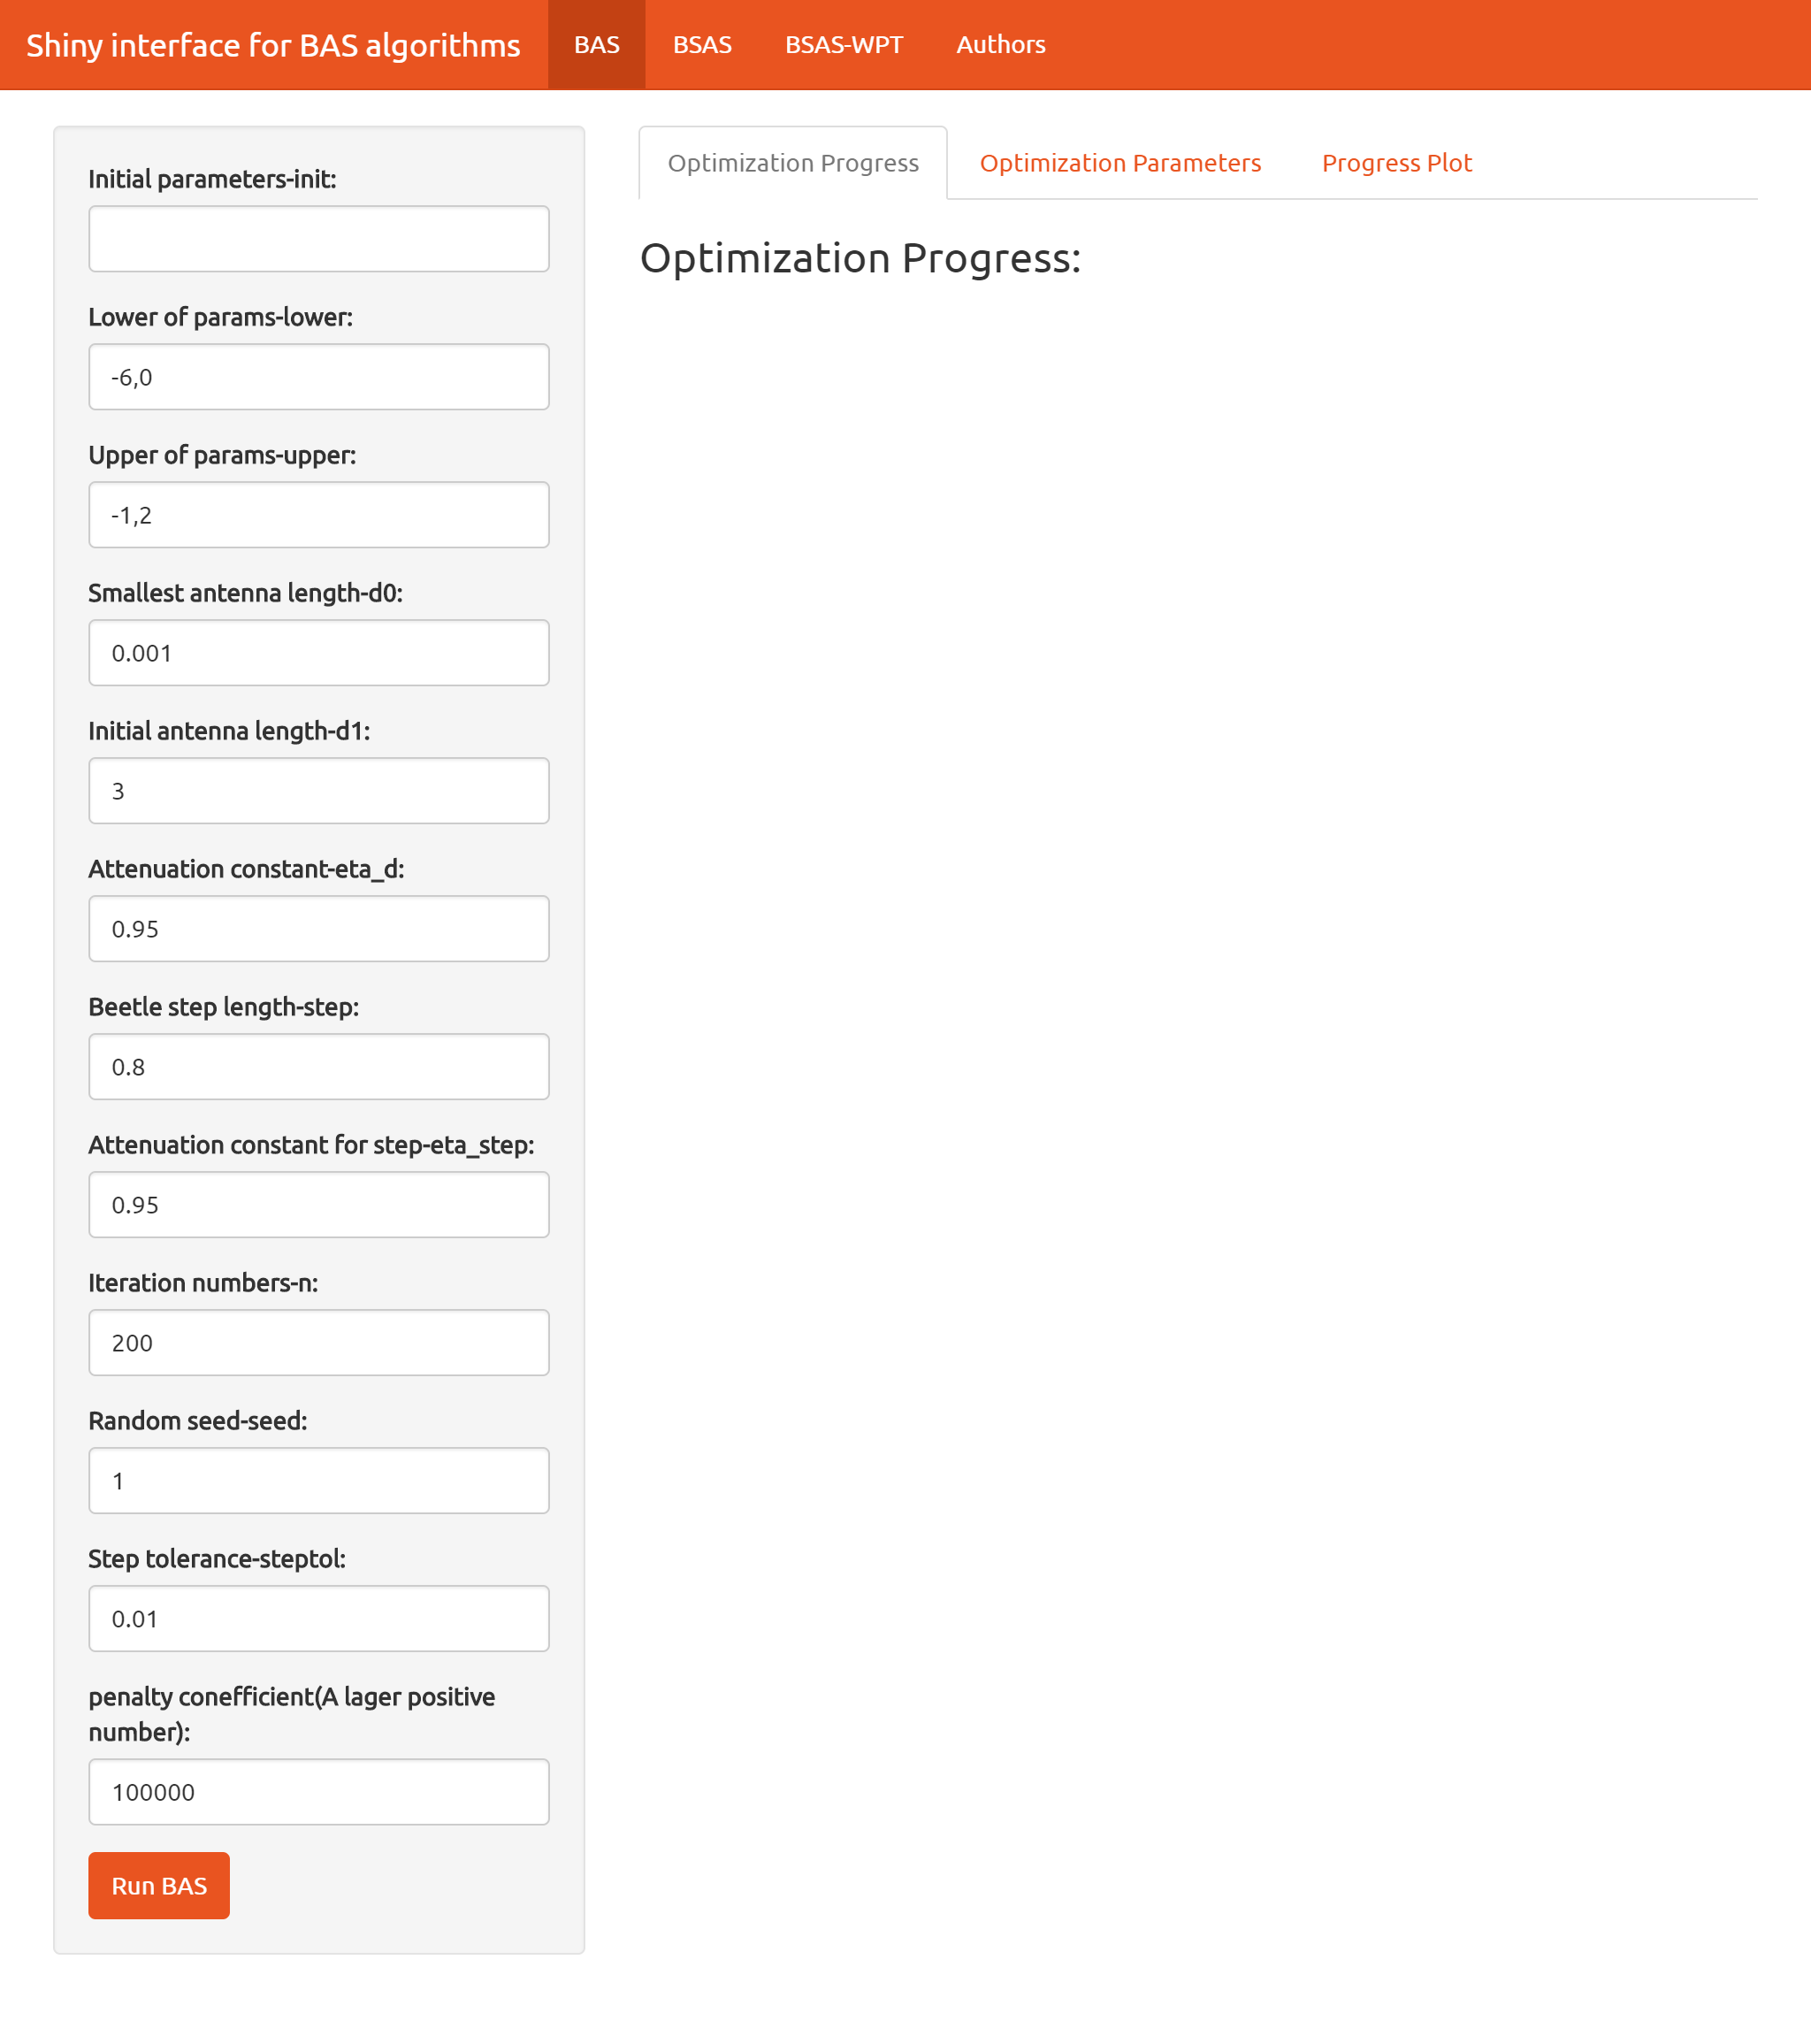
\includegraphics[width=0.95\linewidth]{img/app1} 

}

\caption{shiny interface}\label{fig:basapp}
\end{figure}

左边是固定的参数调节栏,最上方有目前的收录的三种算法可供选择,以及本包的作者信息。右侧也有三个选项,分别是\textbf{优化过程信息},\textbf{优化参数结果}以及\textbf{优化结果可视化}。

按照你的需要,调节好左边的参数信息(第一个参数,也就是初始值\texttt{init},默认为空,也可以指定),然后点击左下方的\texttt{Run\ BAS}键,即可看到如图\ref{fig:basprogress}的内容:

\begin{figure}

{\centering 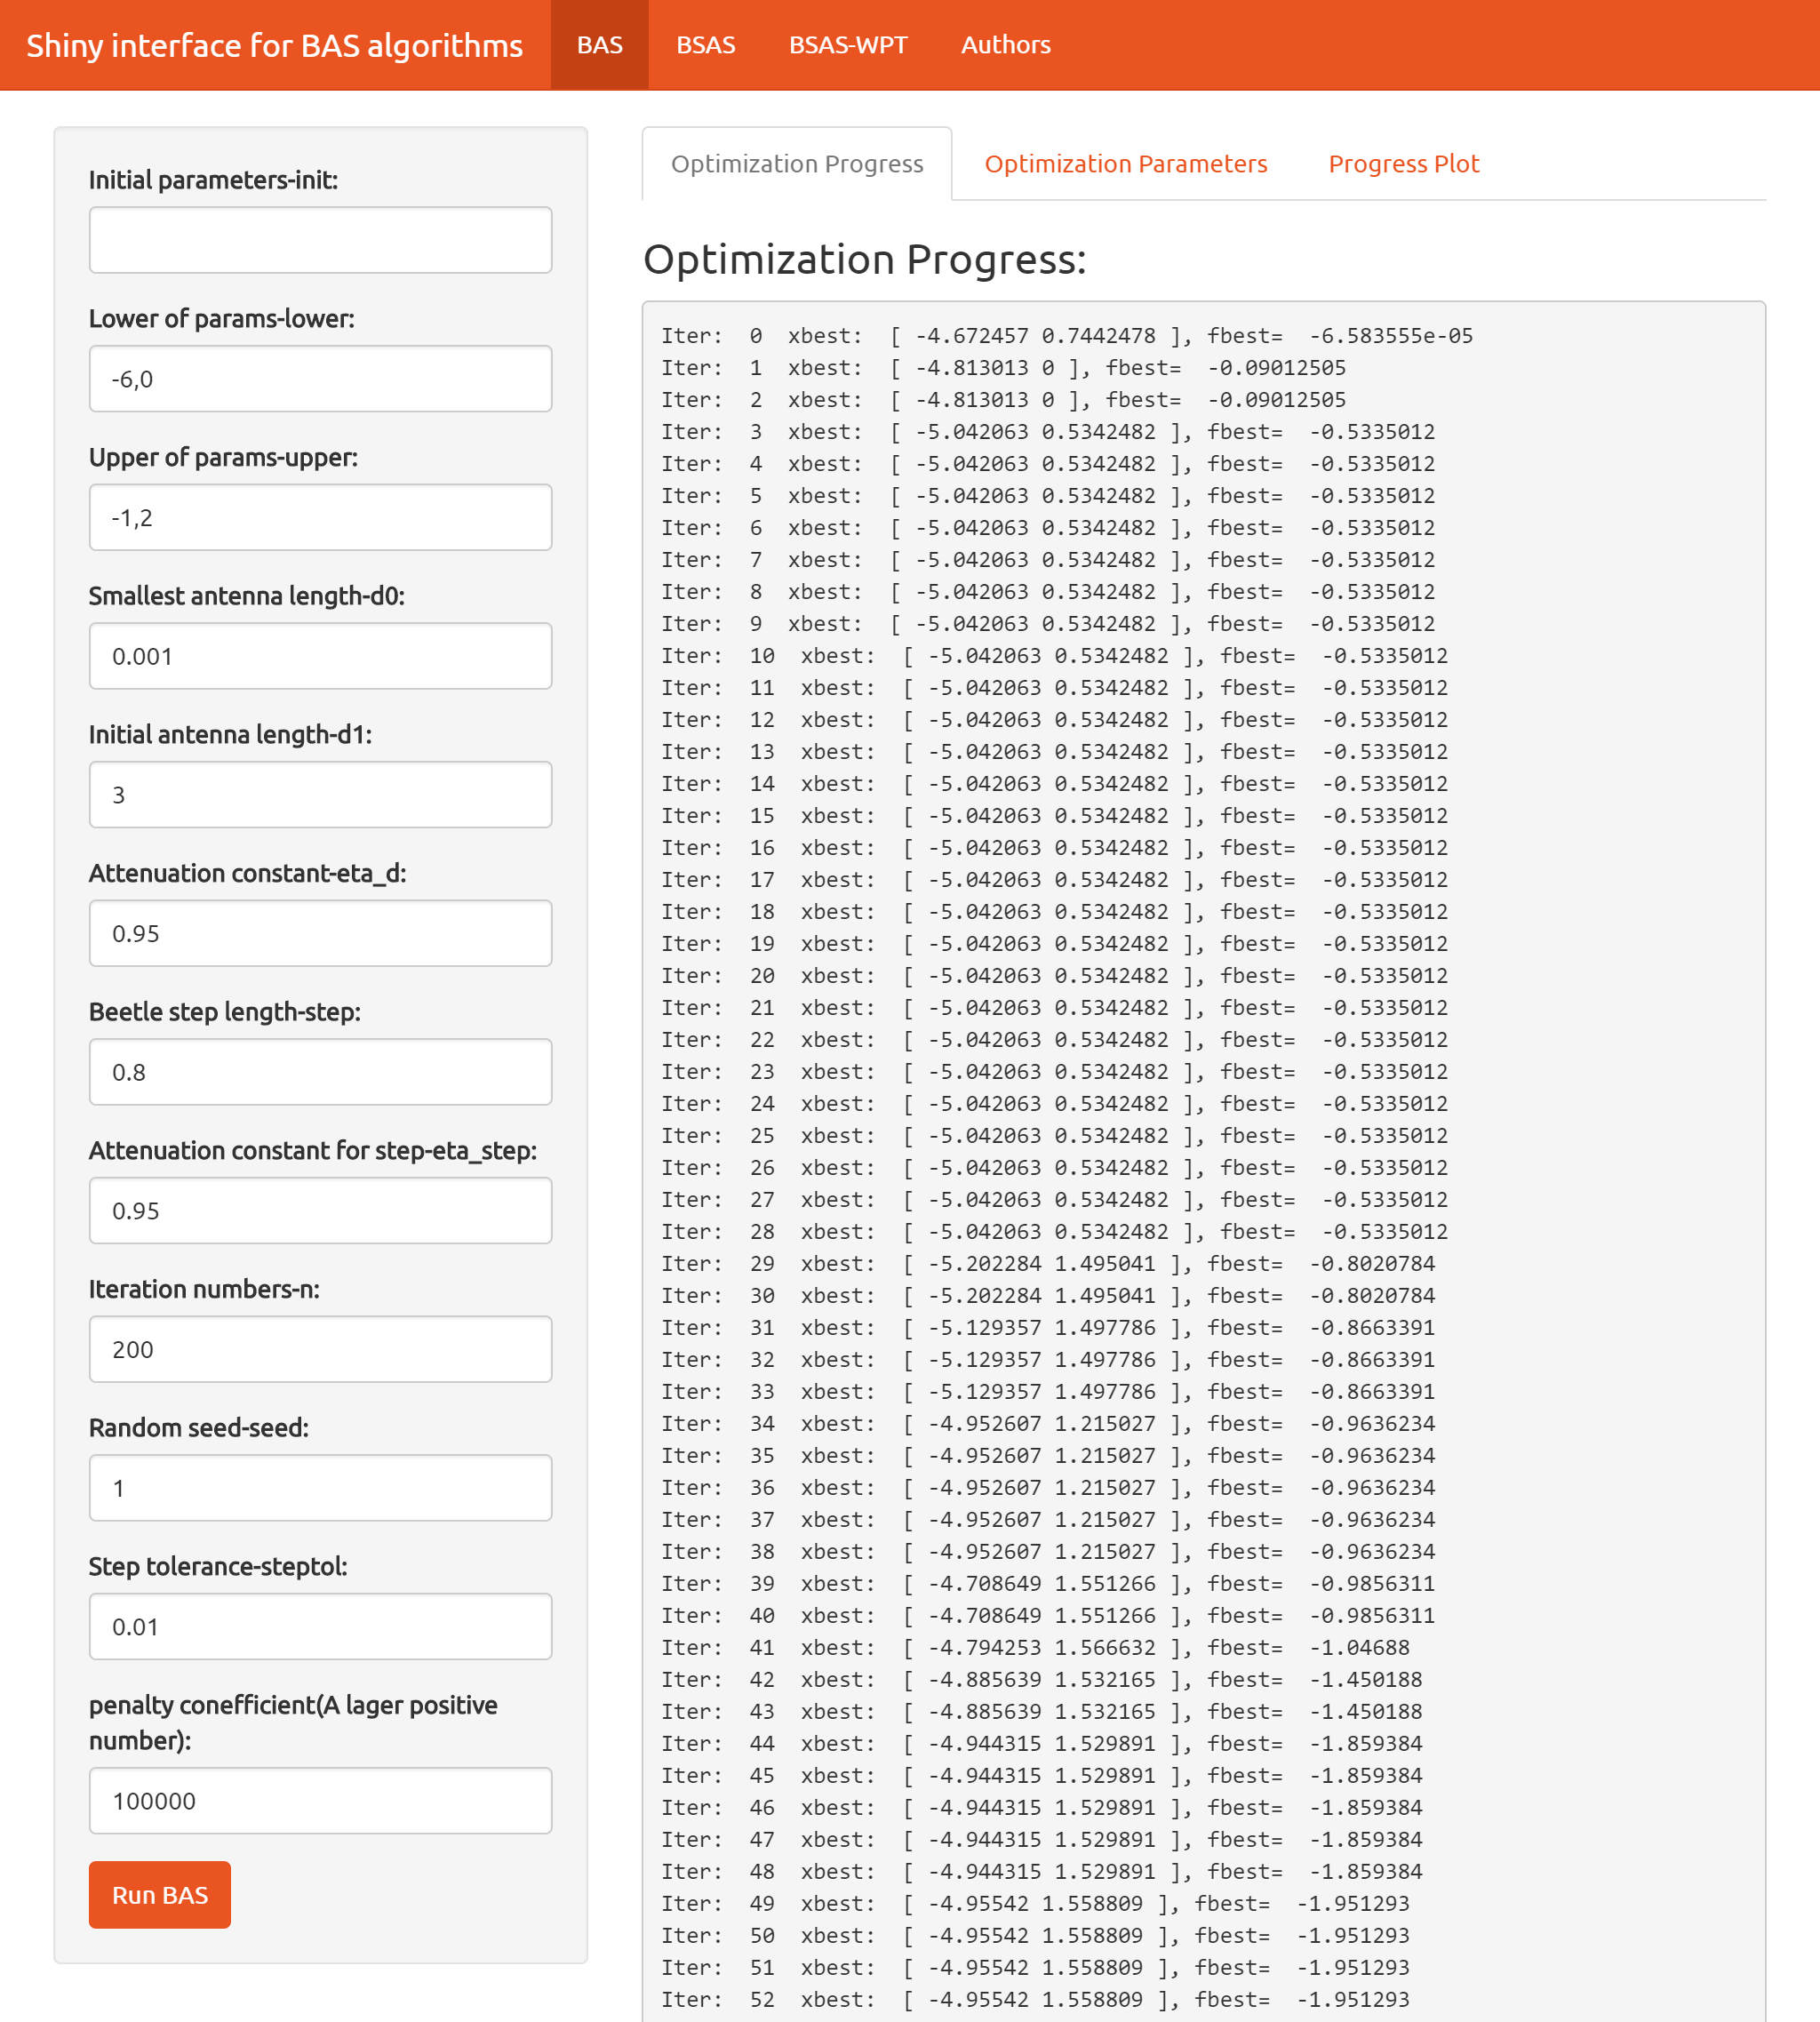
\includegraphics[width=0.95\linewidth]{img/app2} 

}

\caption{optimization progress栏信息}\label{fig:basprogress}
\end{figure}

\begin{quote}
由于回合数较大,因此只截取了部分内容显示。
\end{quote}

分别点击\texttt{Optimization\ Parameters}和\texttt{Progress\ Plot}键,可以看到最后的结果,以及可视化信息,分别如图\ref{fig:basparms}与
\ref{fig:basplot}所示。

\begin{figure}

{\centering 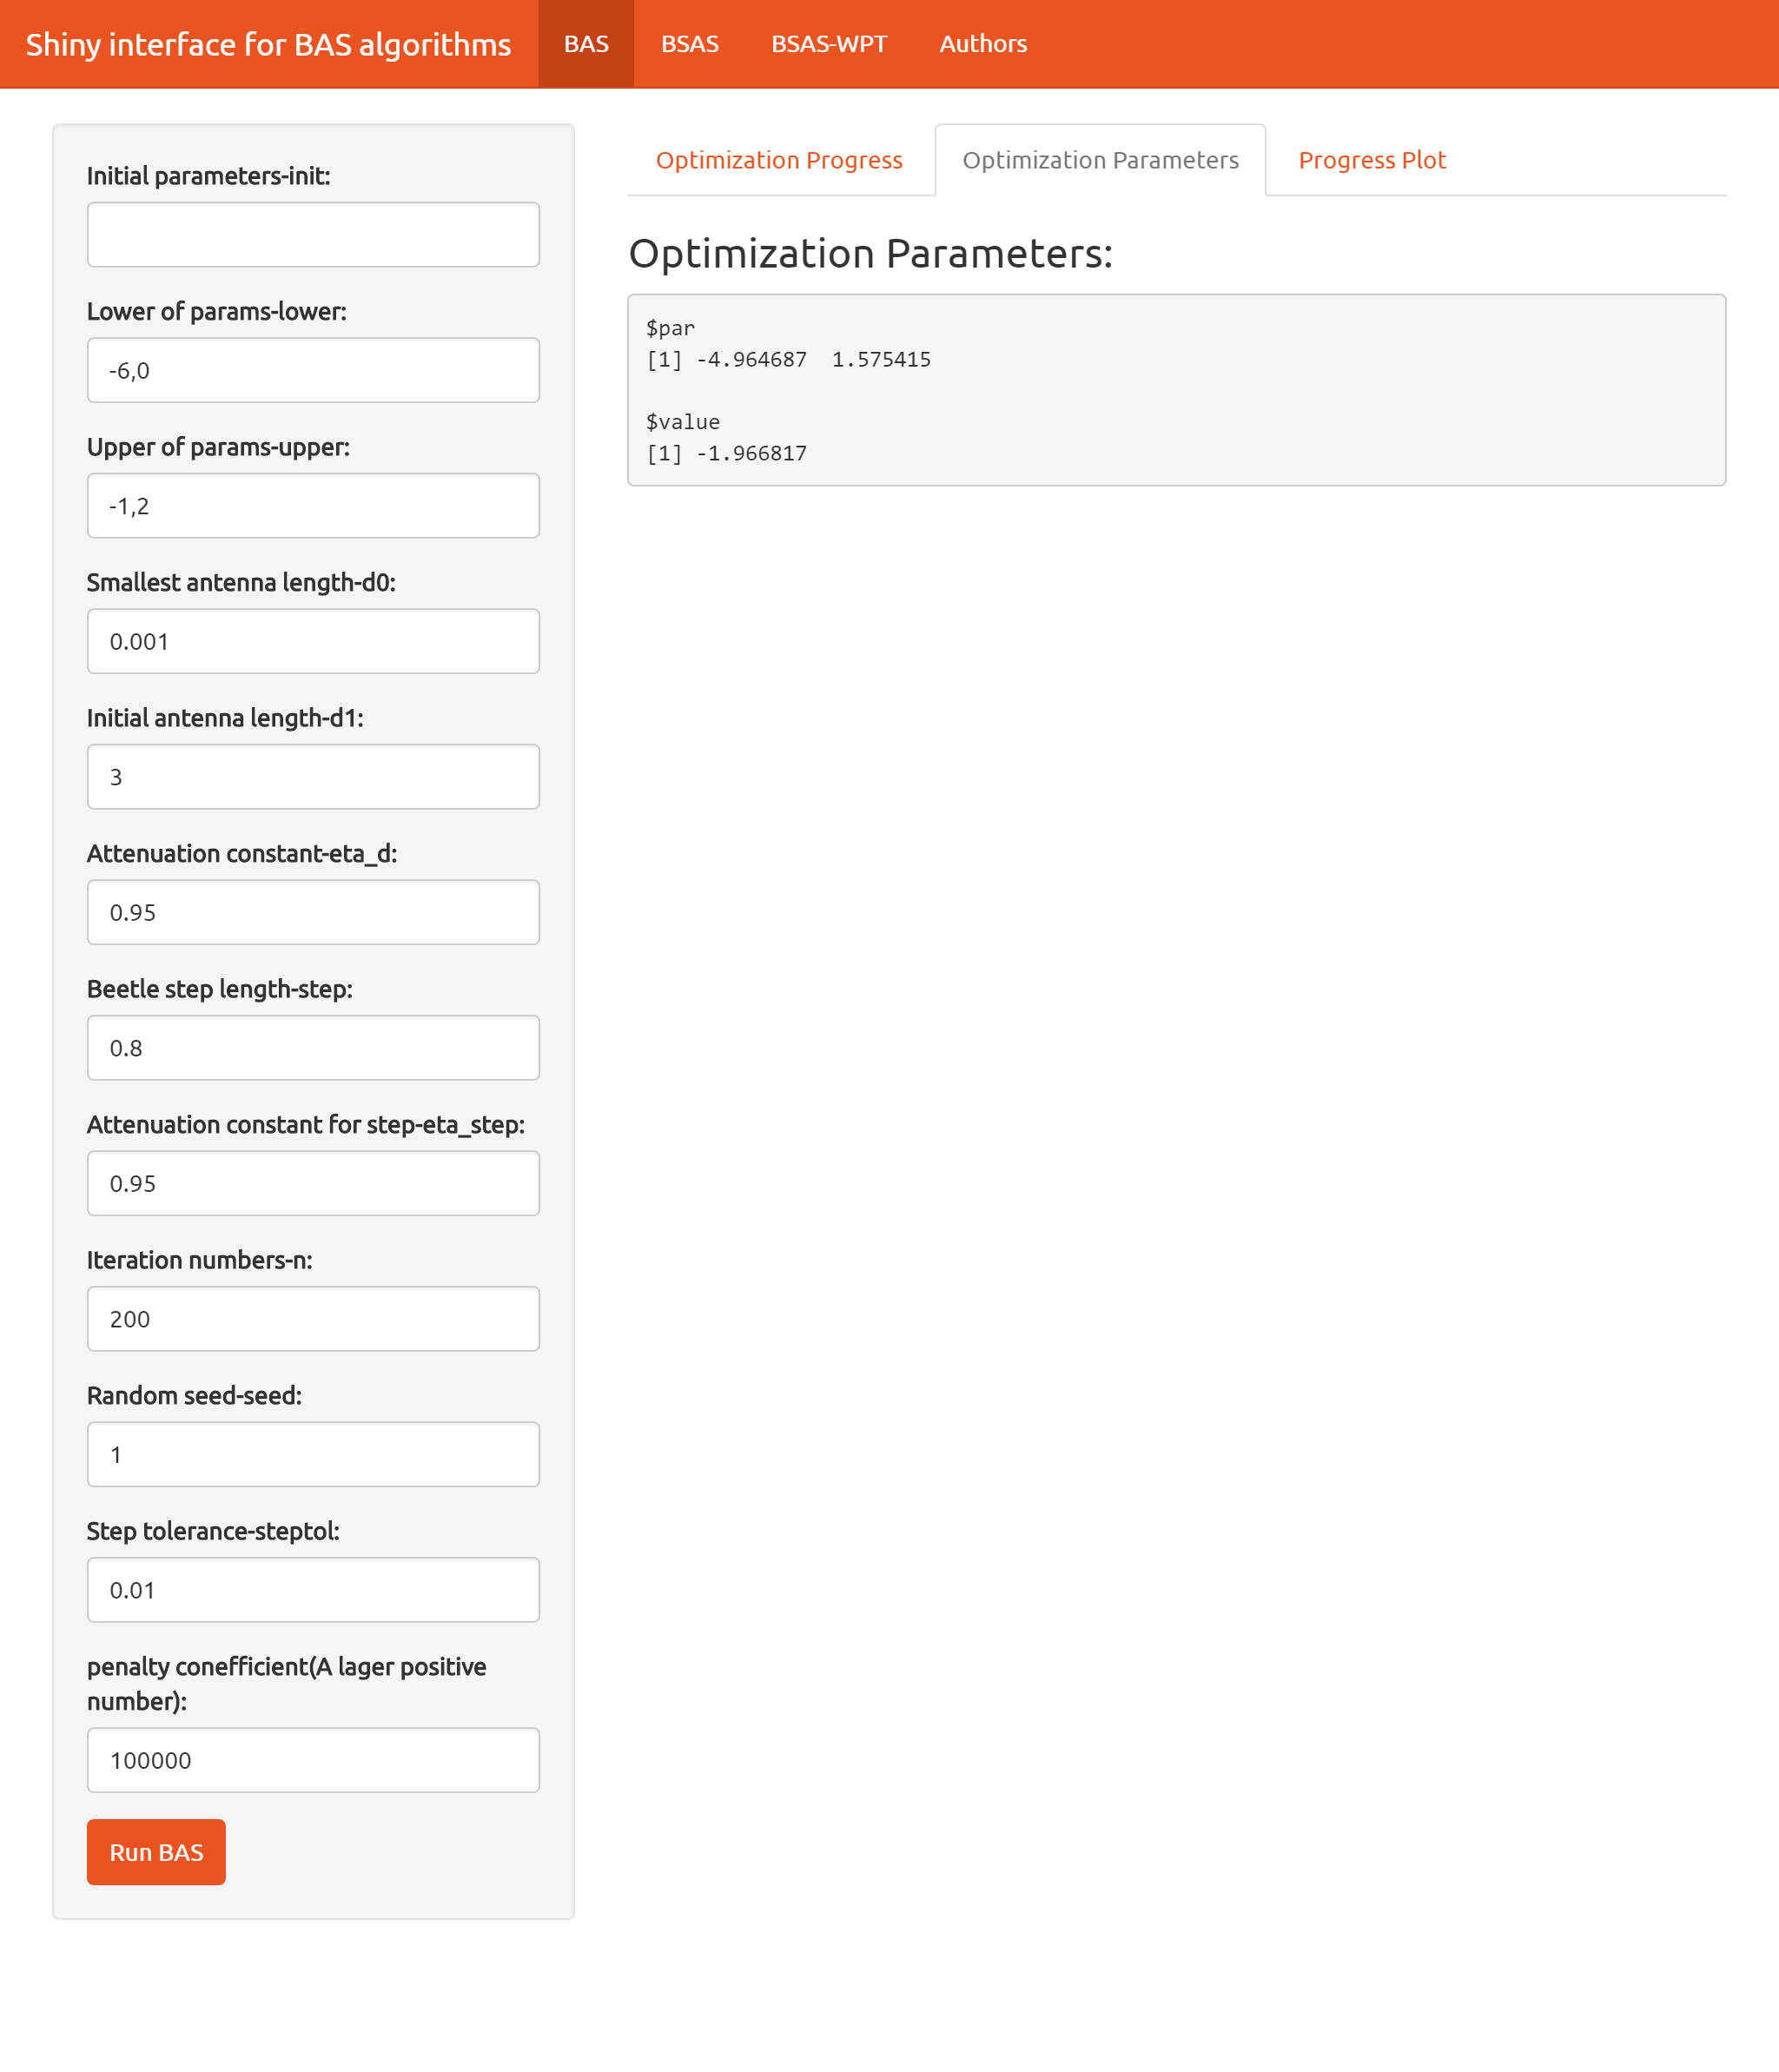
\includegraphics[width=0.95\linewidth]{img/app3} 

}

\caption{Optimization Parameters栏信息}\label{fig:basparms}
\end{figure}

可以看到,窗口的\texttt{\$par}显示的是参数的优化结果,而\texttt{\$value}则是对应的目标函数值。

\begin{figure}

{\centering 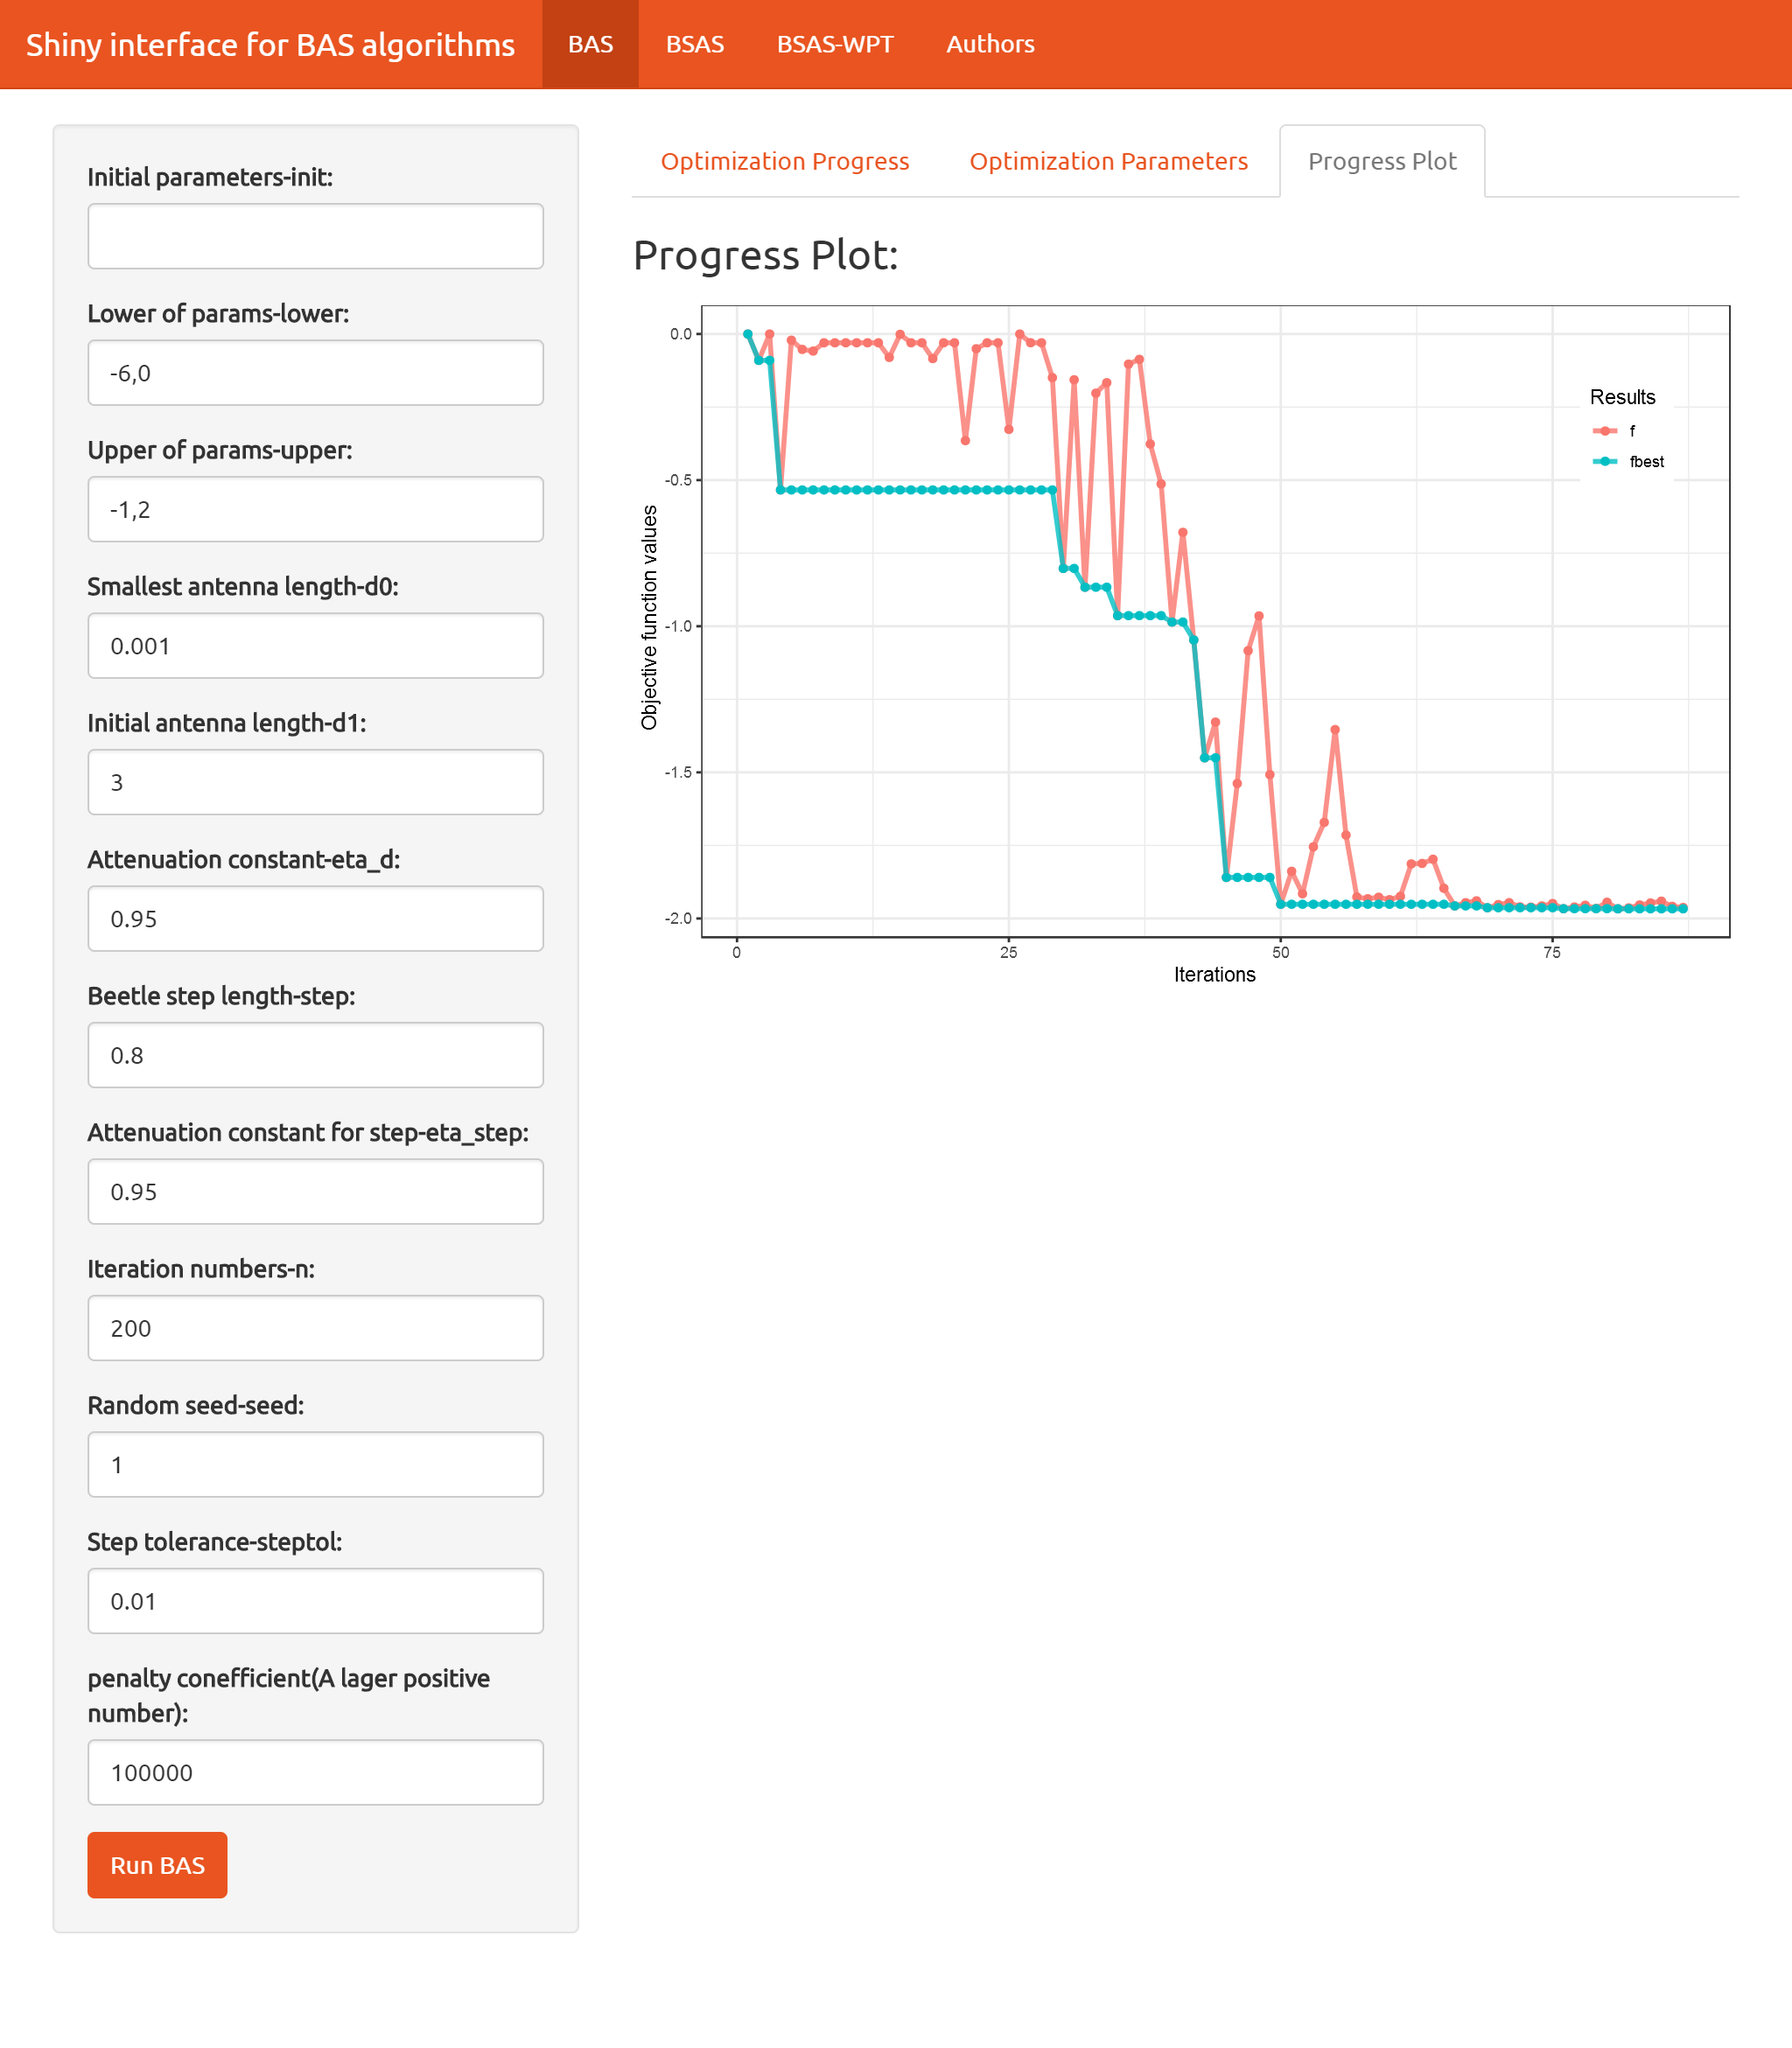
\includegraphics[width=0.95\linewidth]{img/app4} 

}

\caption{Progress Plot栏信息}\label{fig:basplot}
\end{figure}

\texttt{BAS}与其他两种算法有着不同的可视化结果,其并不是基于反馈来控制步长的。因此,图中的两条曲线,红色的为每一回合的目标函数值,而蓝色的为此前回合中最优的目标函数值。

\subsection{Pressure Vessel function}\label{pressure-vessel-function-1}

这次,我们在\texttt{BSAS-WPT}栏下进行界面使用。先在代码中预定义目标函数和约束:

\begin{Shaded}
\begin{Highlighting}[]
\NormalTok{pressure_Vessel <-}\StringTok{ }\KeywordTok{list}\NormalTok{(}
  \DataTypeTok{obj =} \ControlFlowTok{function}\NormalTok{(x)\{}
\NormalTok{    x1 <-}\StringTok{ }\KeywordTok{floor}\NormalTok{(x[}\DecValTok{1}\NormalTok{])}\OperatorTok{*}\FloatTok{0.0625}
\NormalTok{    x2 <-}\StringTok{ }\KeywordTok{floor}\NormalTok{(x[}\DecValTok{2}\NormalTok{])}\OperatorTok{*}\FloatTok{0.0625}
\NormalTok{    x3 <-}\StringTok{ }\NormalTok{x[}\DecValTok{3}\NormalTok{]}
\NormalTok{    x4 <-}\StringTok{ }\NormalTok{x[}\DecValTok{4}\NormalTok{]}
\NormalTok{    result <-}\StringTok{ }\FloatTok{0.6224}\OperatorTok{*}\NormalTok{x1}\OperatorTok{*}\NormalTok{x3}\OperatorTok{*}\NormalTok{x4 }\OperatorTok{+}\StringTok{ }
\StringTok{      }\FloatTok{1.7781}\OperatorTok{*}\NormalTok{x2}\OperatorTok{*}\NormalTok{x3}\OperatorTok{^}\DecValTok{2} \OperatorTok{+}
\StringTok{      }\FloatTok{3.1611}\OperatorTok{*}\NormalTok{x1}\OperatorTok{^}\DecValTok{2}\OperatorTok{*}\NormalTok{x4 }\OperatorTok{+}\StringTok{ }
\StringTok{      }\FloatTok{19.84}\OperatorTok{*}\NormalTok{x1}\OperatorTok{^}\DecValTok{2}\OperatorTok{*}\NormalTok{x3}
\NormalTok{  \},}
  \DataTypeTok{con =} \ControlFlowTok{function}\NormalTok{(x)\{}
\NormalTok{    x1 <-}\StringTok{ }\KeywordTok{floor}\NormalTok{(x[}\DecValTok{1}\NormalTok{])}\OperatorTok{*}\FloatTok{0.0625}
\NormalTok{    x2 <-}\StringTok{ }\KeywordTok{floor}\NormalTok{(x[}\DecValTok{2}\NormalTok{])}\OperatorTok{*}\FloatTok{0.0625}
\NormalTok{    x3 <-}\StringTok{ }\NormalTok{x[}\DecValTok{3}\NormalTok{]}
\NormalTok{    x4 <-}\StringTok{ }\NormalTok{x[}\DecValTok{4}\NormalTok{]}
    \KeywordTok{c}\NormalTok{(}
      \FloatTok{0.0193}\OperatorTok{*}\NormalTok{x3 }\OperatorTok{-}\StringTok{ }\NormalTok{x1,}\CommentTok{#<=0}
      \FloatTok{0.00954}\OperatorTok{*}\NormalTok{x3 }\OperatorTok{-}\StringTok{ }\NormalTok{x2,}
      \FloatTok{750.0}\OperatorTok{*}\FloatTok{1728.0} \OperatorTok{-}\StringTok{ }\NormalTok{pi}\OperatorTok{*}\NormalTok{x3}\OperatorTok{^}\DecValTok{2}\OperatorTok{*}\NormalTok{x4 }\OperatorTok{-}\StringTok{ }\DecValTok{4}\OperatorTok{/}\DecValTok{3}\OperatorTok{*}\NormalTok{pi}\OperatorTok{*}\NormalTok{x3}\OperatorTok{^}\DecValTok{3}
\NormalTok{    )}
\NormalTok{  \}}
\NormalTok{)}
\end{Highlighting}
\end{Shaded}

调用用户界面,注意此时多出了\texttt{constr},也就是约束函数,\texttt{\$}符号在索引列表中的元素时使用:

\begin{Shaded}
\begin{Highlighting}[]
\KeywordTok{run_BAS_App}\NormalTok{(}\DataTypeTok{func =}\NormalTok{ pressure_Vessel}\OperatorTok{$}\NormalTok{obj,}
            \DataTypeTok{constr =}\NormalTok{ pressure_Vessel}\OperatorTok{$}\NormalTok{con)}
\end{Highlighting}
\end{Shaded}

自行调整参数后,用户界面如图\ref{fig:wpt1}所示:

\begin{figure}

{\centering 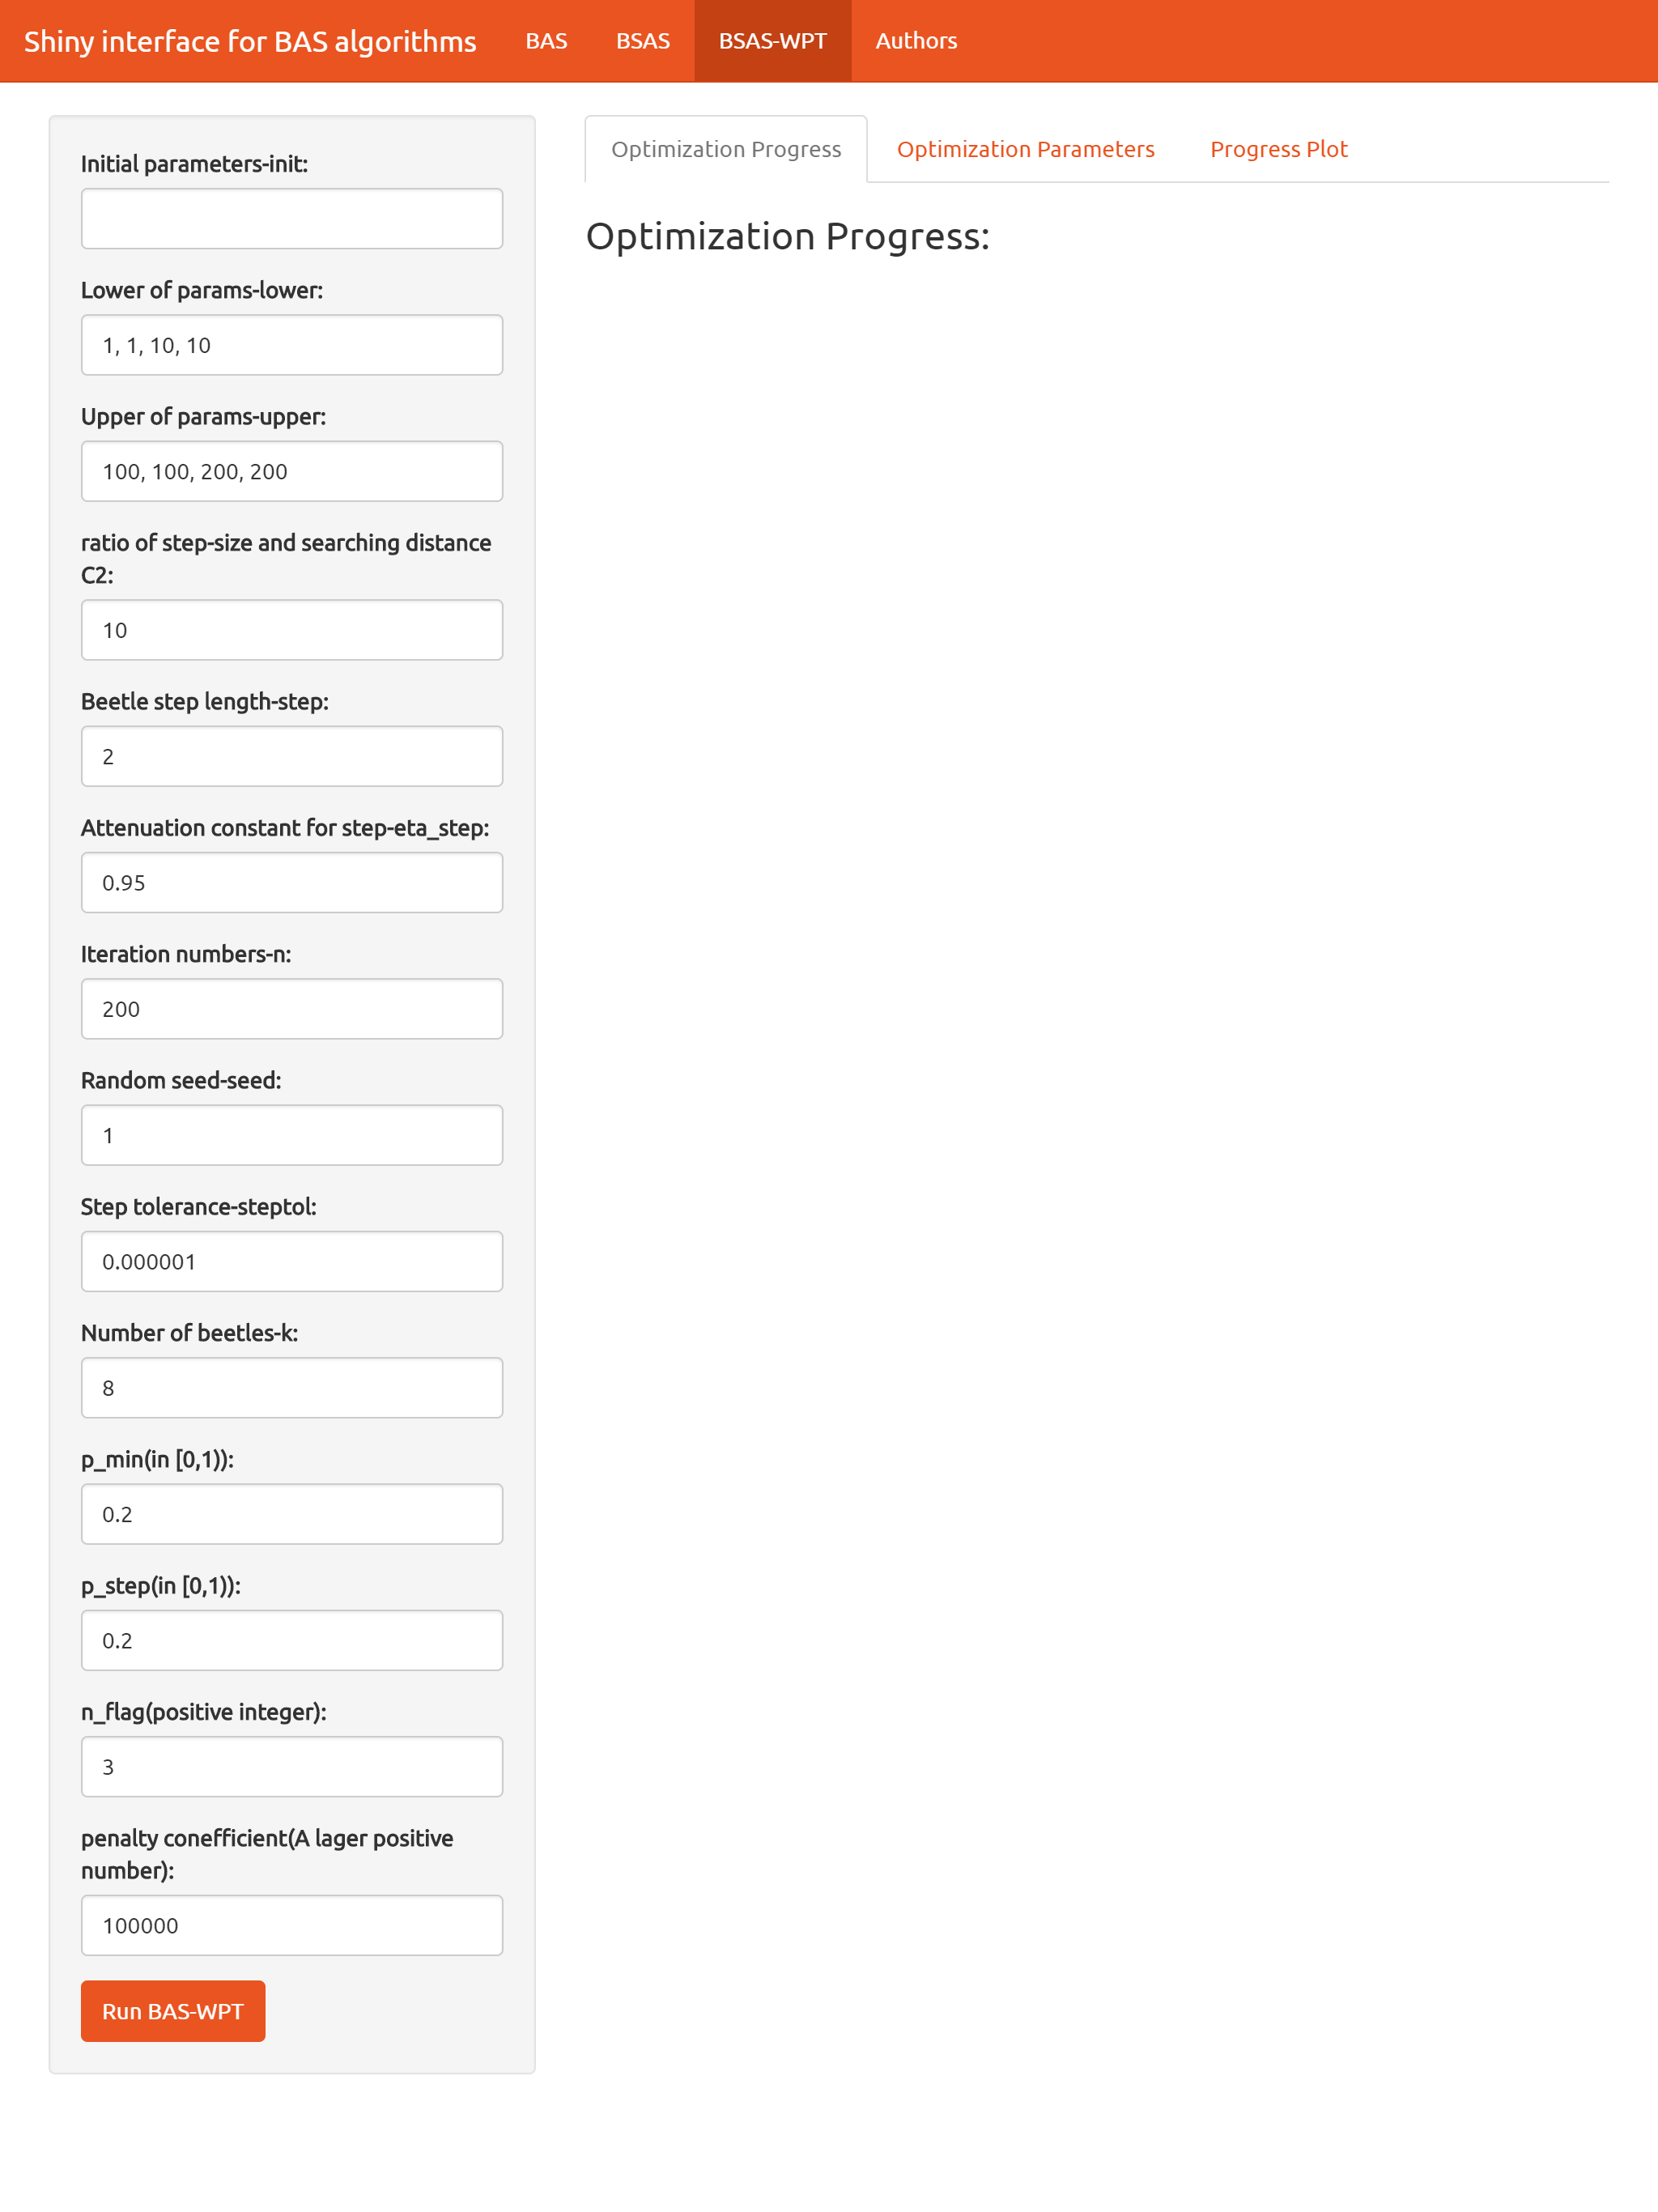
\includegraphics[width=0.95\linewidth]{img/wpt1} 

}

\caption{BSAS-WPT参数调整}\label{fig:wpt1}
\end{figure}

点击\texttt{Run\ BAS-WPT}之后,选择\texttt{optimization\ Parameters}栏目,可以看到优化结果如图\ref{fig:wptparms}所示:

\begin{figure}

{\centering 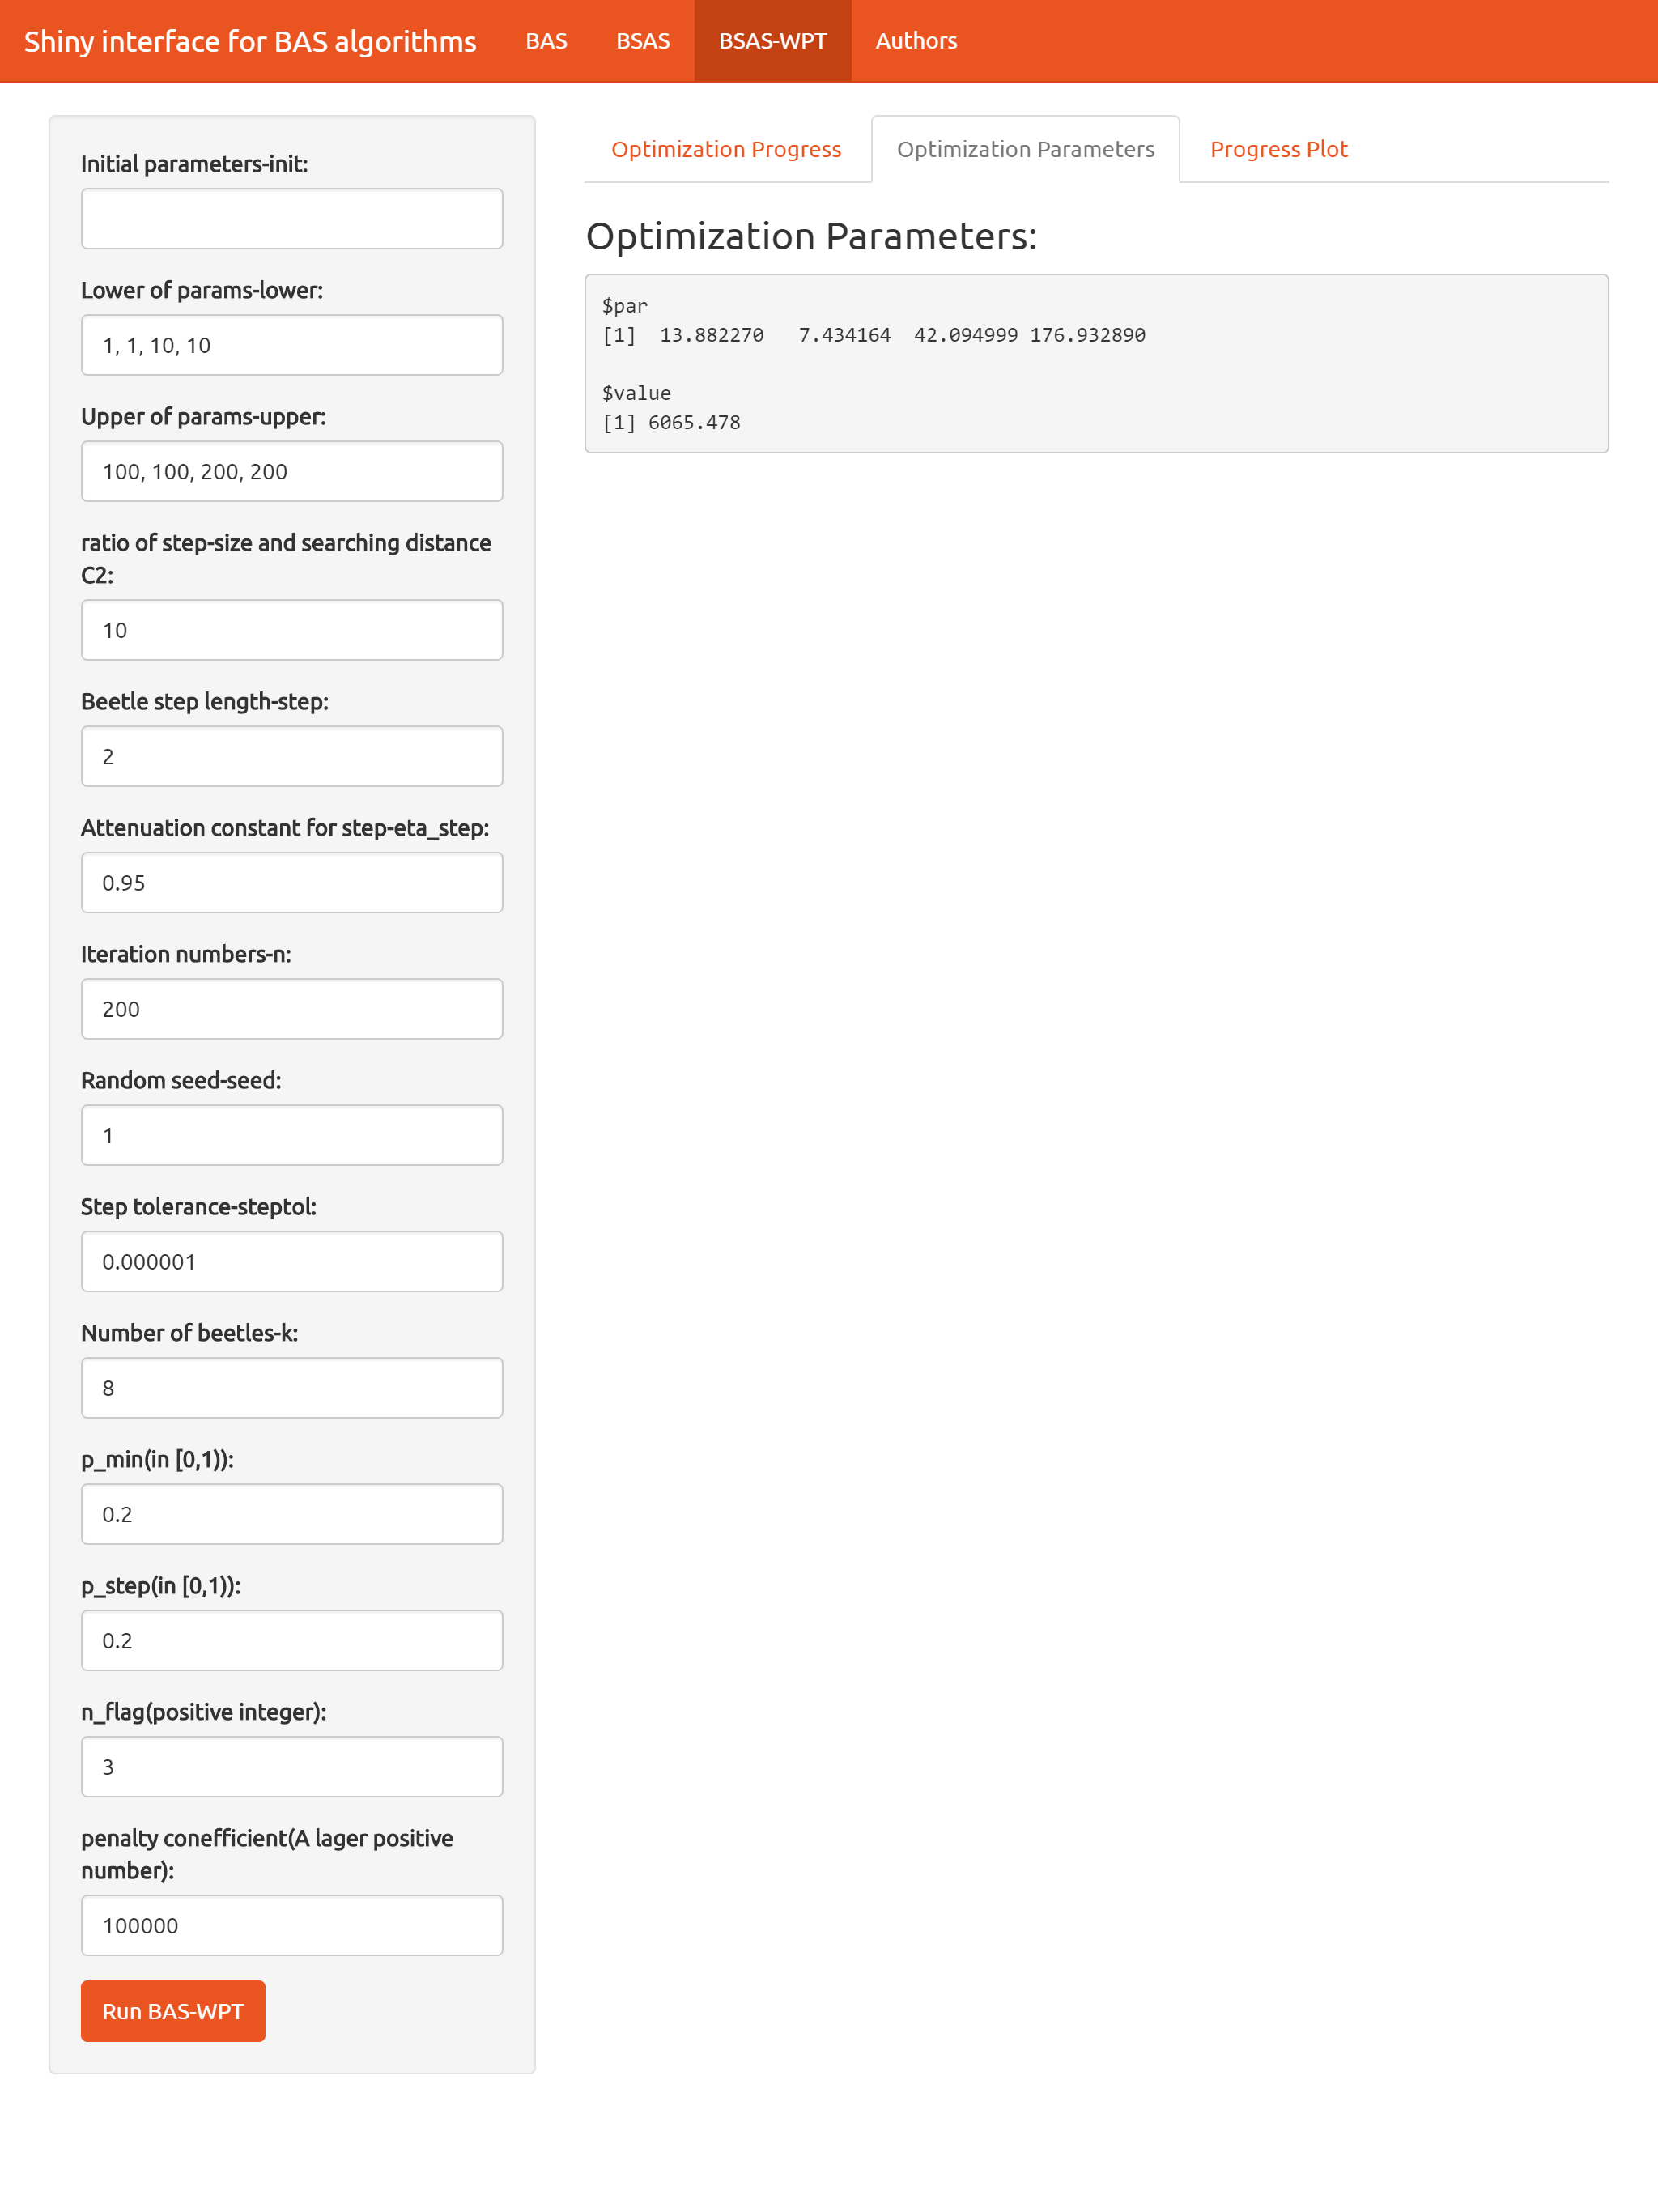
\includegraphics[width=0.95\linewidth]{img/wpt2} 

}

\caption{BSAS-WPT优化结果}\label{fig:wptparms}
\end{figure}

选择\texttt{Progress\ Plot}栏目,过程可视化如图\ref{fig:wptplot}所示:

\begin{figure}

{\centering 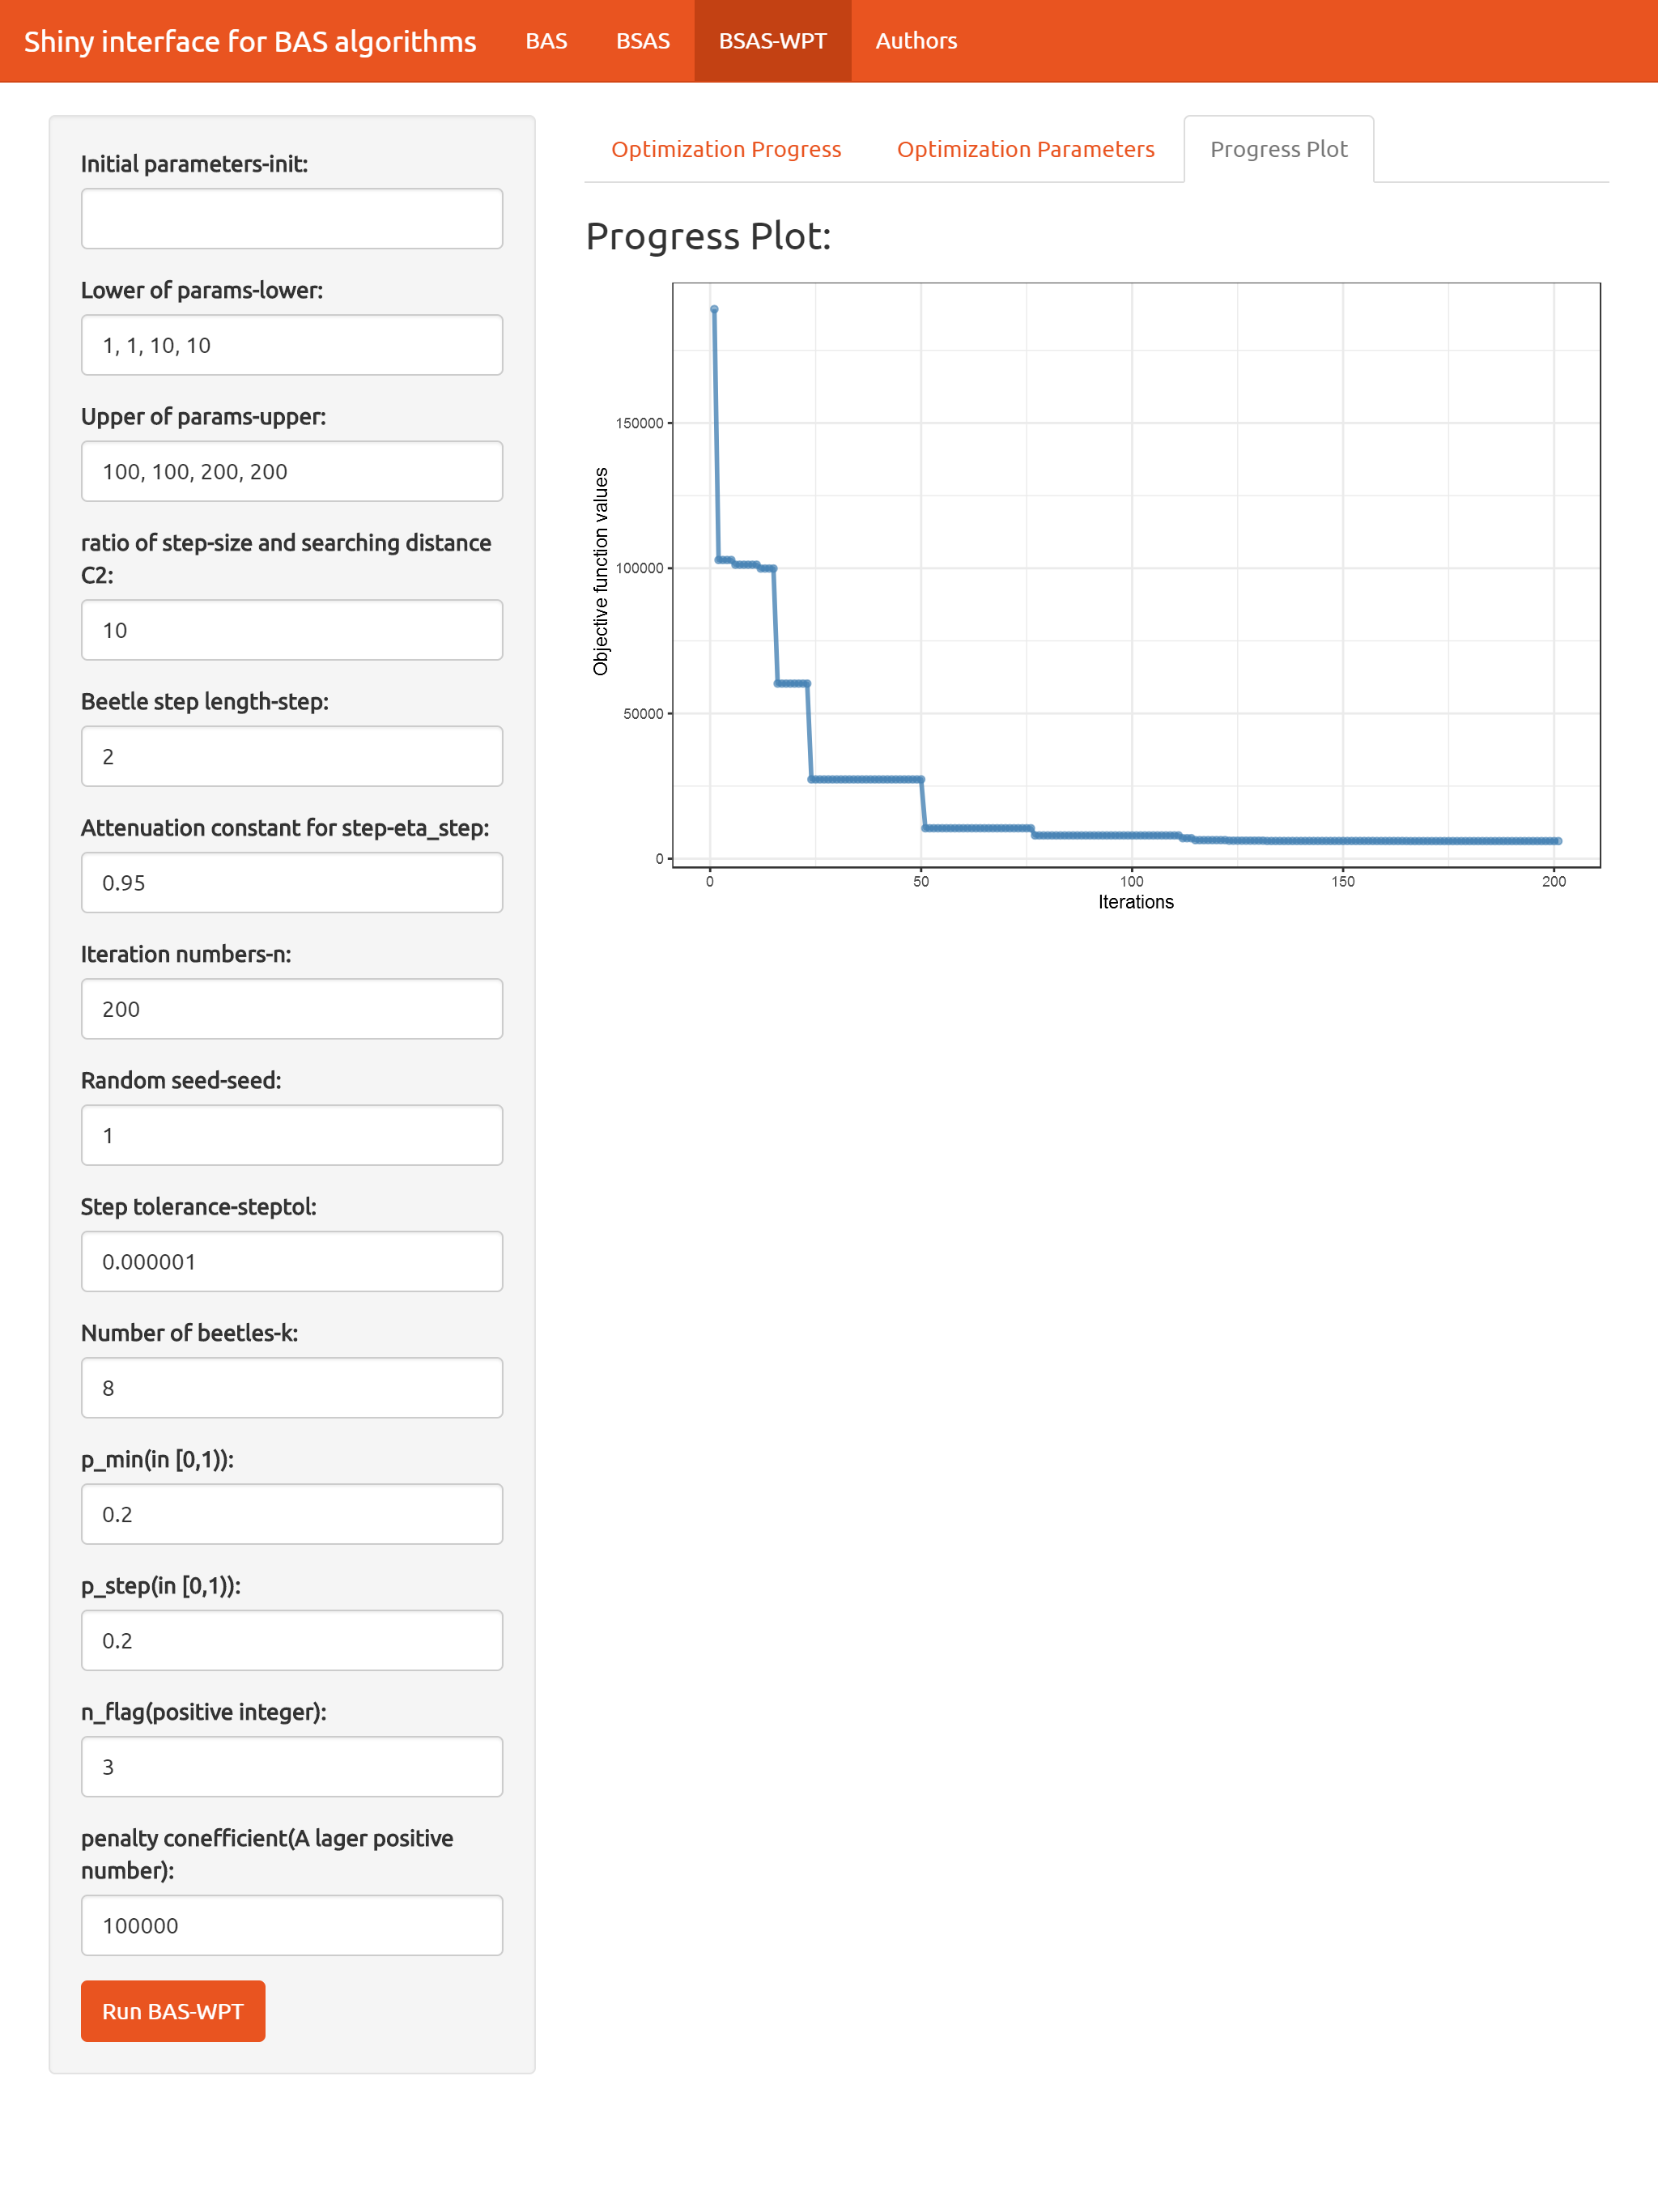
\includegraphics[width=0.95\linewidth]{img/wpt3} 

}

\caption{BSAS-WPT优化过程可视化}\label{fig:wptplot}
\end{figure}

\section{Authors界面}\label{authors}

如果并不想执行任何函数优化,则可以不指定函数和约束。在\texttt{R}里面输入以下代码:

\begin{Shaded}
\begin{Highlighting}[]
\KeywordTok{library}\NormalTok{(rBAS) }\CommentTok{#加载rBAS包}
\KeywordTok{run_BAS_App}\NormalTok{() }\CommentTok{#直接调用函数}
\end{Highlighting}
\end{Shaded}

可以看到\texttt{rBAS}的用户界面,里面有关于\texttt{rBAS}的作者信息,如图\ref{fig:author}所示。

\begin{figure}

{\centering 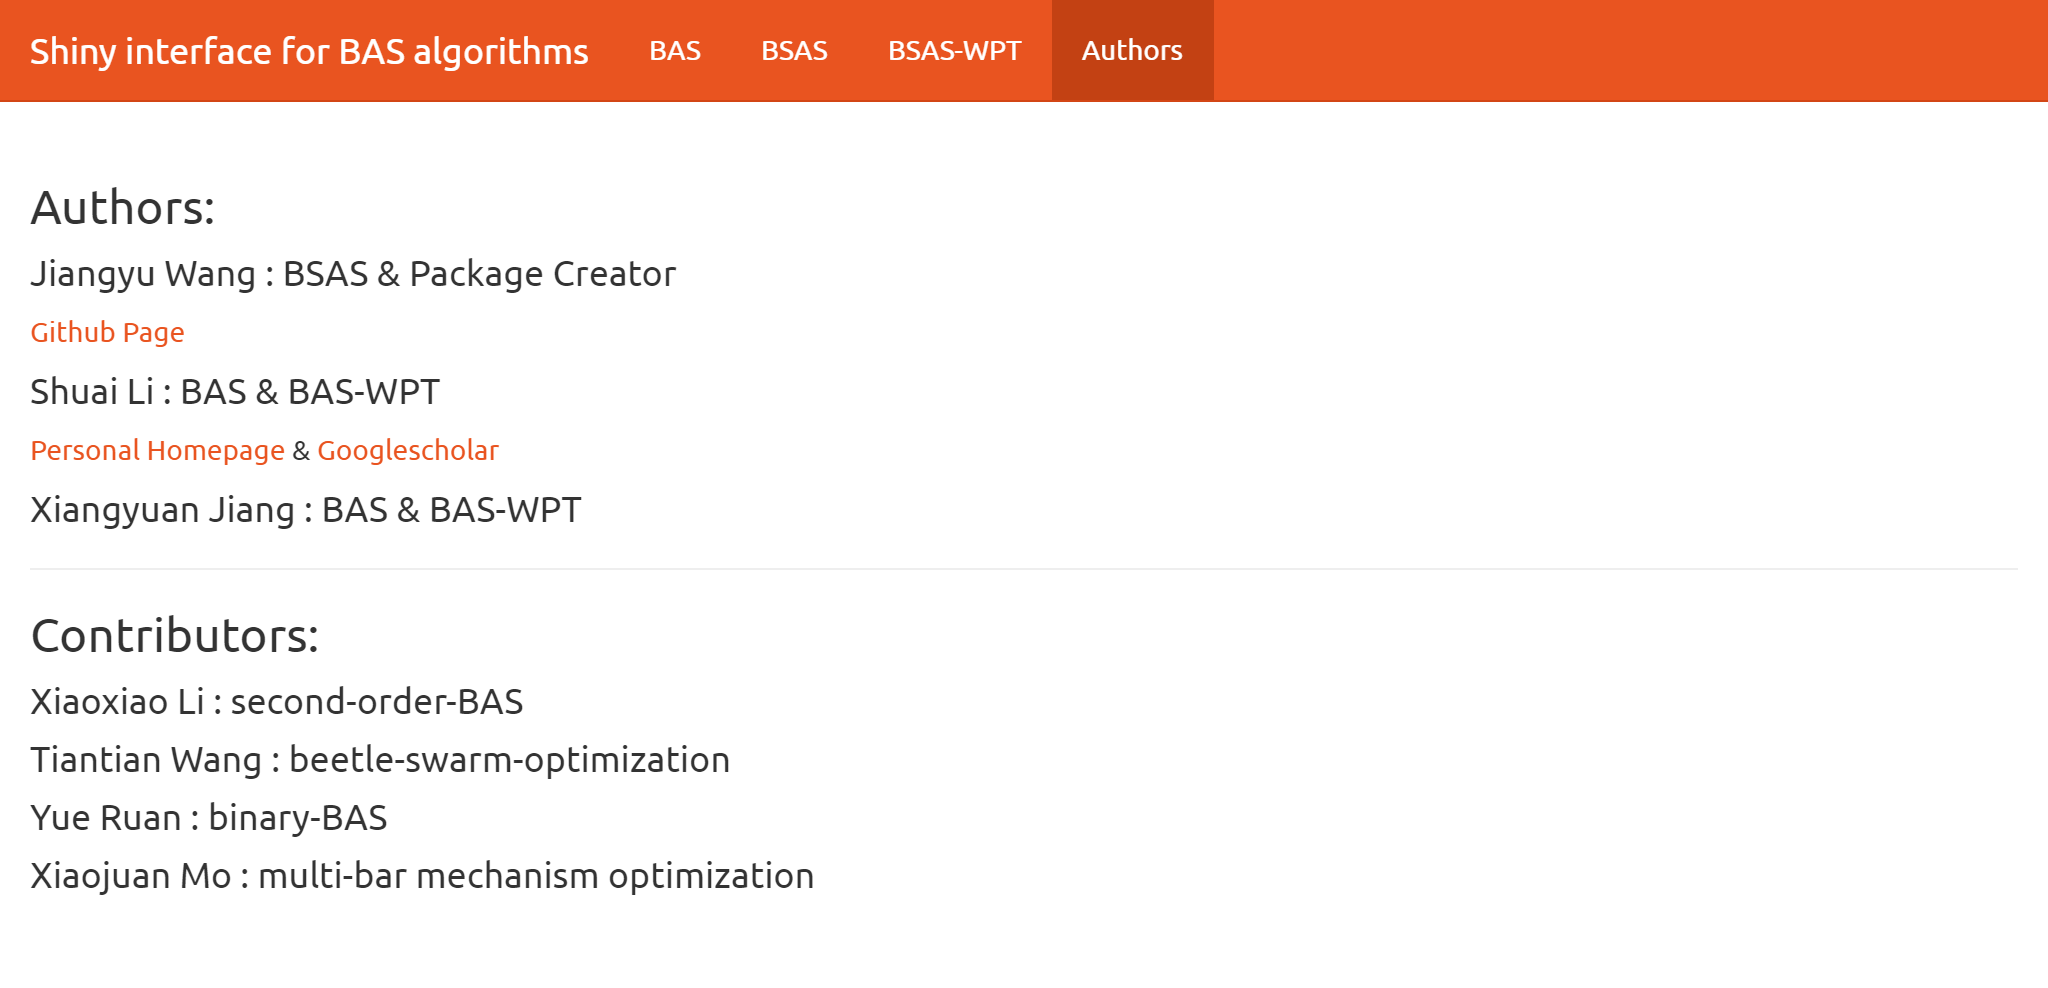
\includegraphics[width=1\linewidth]{img/author} 

}

\caption{用户界面作者信息}\label{fig:author}
\end{figure}

如果大家对该项目有兴趣,参与了包的开发,或者\texttt{BAS}算法应用案例的提出。我会在征得当事人同意的情况下,将名字加入该界面:)。

\chapter{BAS案例一:多杆机构优化问题}\label{examples}

说明:由于自身专业知识局限,在整理转述各位研究者或贡献者所提供的材料时,我可能无法准确地表达出对应领域的知识要点。避免言多必失,我仅仅做简要的翻译或者是介绍。对于读者而言,如果觉得并不能解你之疾,或没有\textbf{挠到痒处},建议直接和对应的作者联系。对于贡献者而言,如果我表述有误,欢迎提出建议,或者在github上\texttt{pull\ request}。

\begin{quote}
由群友莫小娟博士研究生提供案例。
\end{quote}

由于案例均为各位热心的同学提供,均为自己的研究。因此,希望大家要引用其中的结果时,可以引用对应同学的文章。此外,也请大家转载时注明来源。

\section{背景}

\subsection{四连杆机构(Four-bar linkage mechanism)}\label{bars4}

四连杆机构如图\ref{fig:fourbars}所示:

\begin{figure}

{\centering 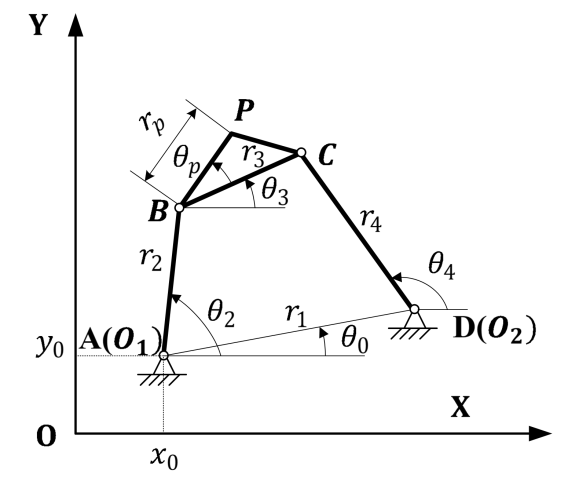
\includegraphics[width=0.7\linewidth]{img/bars4} 

}

\caption{四连杆机构示意}\label{fig:fourbars}
\end{figure}

基于闭环矢量方程,推导出节点位置。推导过程如式\eqref{eq:bars4loop1}至式\eqref{eq:bars4loop4}:

\begin{equation}
\mathbf{\text{Loop:}}   r_1e^{i\theta_0} + r_4e^{i\theta_4} - r_2e^{i\theta_2} -r_3e^{i\theta_3} = 0\\
\label{eq:bars4loop1}
\end{equation}

\begin{equation}
\begin{cases} 
r_1cos(\theta_0) + r_4cos(\theta_4)-r_2cos(\theta_2)-r_3cos(\theta_3)=0 \\ 
r_1sin(\theta_0) + r_4sin(\theta_4)-r_2sin(\theta_2)-r_3sin(\theta_3)=0
\end{cases}
\label{eq:bars4loop2}
\end{equation}

\begin{equation}
\begin{split}
&\theta_3 =2atan(\frac{-A\pm\sqrt{2}{A^2-4BC}}{2B})+\theta_0\\
&A = cos(\theta_2 - \theta_0)-K_1+K_2cos(\theta_2-\theta_0)+K_3\\
&B = -2sin(\theta_2-\theta_0), F=K_1+(K_2-1)cos(\theta_2-\theta_0)+K_3\\
&K_1 = r_1/r_2,K_2=r_1/r_3,K_3=(r_4^2-r_1^2-r_2^2-r_3^2)/(2r_2r_3)\\
\end{split}
\label{eq:bars4loop3}
\end{equation}

\begin{equation}
\begin{cases} 
x_p=x_0+r_2cos(\theta_2)+r_pcos(\theta_3+\theta_p) \\ 
y_p=y_0+r_2sin(\theta_2)+r_psin(\theta_3+\theta_p)
\end{cases}
\label{eq:bars4loop4}
\end{equation}

\subsection{六连杆机构(Stephenson III Six-bar linkage
mechanism)}\label{bars6}

六连杆机构如图\ref{fig:sixbars}所示:

\begin{figure}

{\centering 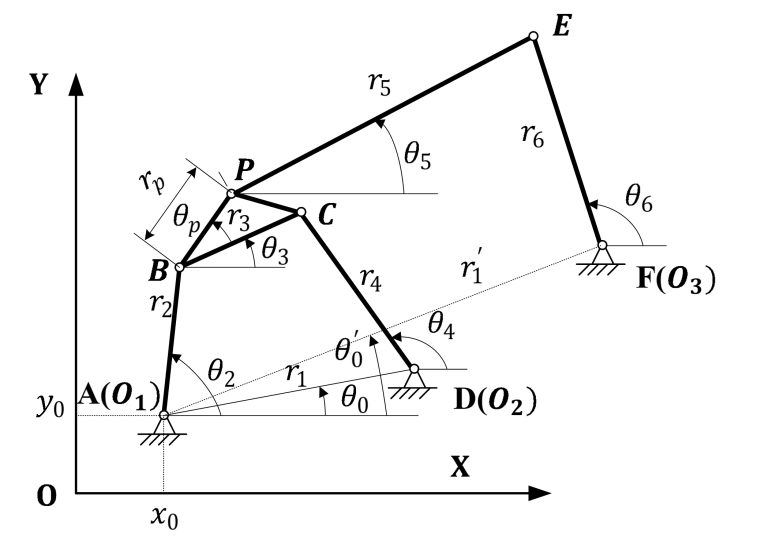
\includegraphics[width=0.7\linewidth]{img/bars6} 

}

\caption{六连杆机构示意}\label{fig:sixbars}
\end{figure}

基于闭环矢量方程,推导出节点位置和外部链接角度。推导过程如式\eqref{eq:bars6loop1}至式\eqref{eq:bars6loop2}:

\begin{equation}
\begin{split}
&\mathbf{\text{Loop1:}}   r_1e^{i\theta_0} + r_4e^{i\theta_4} - r_2e^{i\theta_2} -r_3e^{i\theta_3} = 0\\
&\mathbf{\text{Loop2:}}   r_1'e^{i\theta_0'} + r_6e^{i\theta_6} - r_2e^{i\theta_2} -r_pe^{i(\theta_3+\theta_p)}-r_5e^{i\theta_5} = 0\\
\end{split}
\label{eq:bars6loop1}
\end{equation}

\begin{equation}
\begin{split}
\text{Loop1:}\\
&\alpha = r_2cos(\theta_2) - r_1cos(\theta_0), \beta = r_2sin(\theta_2)-r_1sin(\theta_0) \\
&\gamma = (r_4^2+\alpha^2+\beta^2-r_3^2)/(2r_4),\lambda=atan2(\alpha,\beta)\\
&\theta_4 = atan(cos(\lambda)\gamma/\beta,\{1-(cos(\lambda)\gamma/\beta)^2\}^{1/2})-\lambda\\
&\theta_3=atan2(r_4sin(\theta_4)-\beta,r_4cos(\theta_4)-\alpha)\\
\text{Loop2:}\\
&\alpha_1 = r_2cos(\theta_2)+r_pcos(\theta_3+\theta_p)-r_6cos(\theta_6)\\
&\beta_1=r_2sin(\theta_2)+r_psin(\theta_3+\theta_p)-r_6sin(\theta_6)\\
&\gamma_1=(r_6^2+\alpha_1^2+\beta_1^2-r_5^2)/(2r_6),\lambda_1=atan2(\alpha_1,\beta_1)\\
&\theta_6=atan2(cos(\lambda)\gamma_1/\beta_1,-\{1-(cos(\lambda_1)\gamma_1/\beta_1)^{2}\}^{1/2}) - \lambda_1\\
&\theta_5 = atan2(r_6sin(\theta_6)-\beta_1,r_6cos(\theta_6)-\alpha_1)
\end{split}
\label{eq:bars6loop2}
\end{equation}

于是,可以得到节点位置如式\eqref{eq:bars6loop3}:

\begin{equation}
\begin{cases} 
x_A = x_0,y_A = y_0 \\
x_D = x_0+r_1cos(\theta_0),y_D = y_0+r_1sin(\theta_0)\\
x_F = x_0+r_1'cos(\theta_0'),x_F = x_0 + r_1'sin(\theta_0')\\
x_p = x_0 + r_2cos(\theta_2) + r_pcos(\theta_3+\theta_p)\\
y_P = y_0 + r_2sin(\theta_2)+r_Psin(\theta_3+\theta_p)\\
\end{cases}
\label{eq:bars6loop3}
\end{equation}

\section{优化问题}

\subsection{四连杆机构}\label{bars4optim}

四杆机构的优化问题可以用式\eqref{eq:optim4bars}表示。

\begin{equation}
\begin{split}
\text{min   } &\sum_{i=1}^N[(P_{Xd}^i-P_X^i)^2+(P_{Yd}^i-P_Y^i)^2]+M_1h_1(x)+M_2h_2(x)\\
\text{where } & x_i\in [l_{min}^i,l_{max}^i] \quad \forall x_i \in X,\\
&X=[r_1,r_2,r_3,r_4,r_p,\theta_p,\theta_0,x_0,y_0,\theta_2^1,\cdots,\theta_2^N]\\
\end{split}
\label{eq:optim4bars}
\end{equation}

其中,

\begin{equation}
h_1(x) = \begin{cases}
1, & \text{the Grashof condition false}\\
0, & \text{the Grashof condition true}
\end{cases}
\label{eq:hx1}
\end{equation}

\begin{equation}
h_2(x) = \begin{cases}
1, & \text{the sequence condition of the crank angle false}\\
0, & \text{the sequence condition of the crank angle true}
\end{cases}
\label{eq:hx2}
\end{equation}

\(h_1(X)\) 和 \(h_2(X)\)
分别用于评估曲柄存在条件(\texttt{Grashof\ Condition})以及曲柄角度(顺时针或逆时针)的顺序情况。\(M_1\)
和 \(M_2\)分别是对应的惩罚系数。\(X\) 为设计参数。

\subsection{六连杆机构}\label{bars6optim}

\begin{equation}
\begin{split}
\text{min   } &\sum_{i=1}^N[(P_{Xd}^i-P_X^i)^2+(P_{Yd}^i-P_Y^i)^2]+\sum_{i=1}^M[(\theta_{6d}^i-\theta_6^i)^2]\\
&+M_1h_1(x)+M_2h_2(x)+M_3h_3(X)\\
\text{where } & x_i\in [l_{min}^i,l_{max}^i] \quad \forall x_i \in X,\\
&X=[r_1,r_2,r_3,r_4,r_5,r_6,r_p,\theta_p,\theta_0,x_0,y_0,\theta_2^1,\cdots,\theta_2^N]\\
\end{split}
\label{eq:optim6bars}
\end{equation}

其中,\(h_1(X)\) 与 \(h_2(X)\) 同式\eqref{eq:hx1}与\eqref{eq:hx2},
\(h_3(X)\)如式\eqref{eq:hx3}:

\begin{equation}
h_3(x) = \begin{cases}
1, & \text{non-violation of transmission angle false}\\
0, & \text{non-violation of transmission angle true}
\end{cases}
\label{eq:hx3}
\end{equation}

\(h_3(X)\)
所表示的是,是否没有违背传动角(超过20°)的约束。同样地,\(M_3\)
为对应的惩罚系数。

\section{优化理论}

案例所使用的算法是\textbf{标准化的群体天牛算法}。有意思的是,此处群体天牛算法,和\texttt{rBAS}包的\texttt{BSASoptim}的算法极为类似。这也说明,加入群体智能策略,会使得\texttt{BAS}对于复杂问题寻优能力增强。

联系在于:此案例使用的群体天牛,是在每回合,对于天牛探索方向数的提升。即,每回合生成多个随机的方向,在这些方向上,派出天牛进行试探。这点和\texttt{BSAS}保持一致,可以理解为,\textbf{如果天牛不止有一对须,而是有多对,那每回合探索的方向也会有多个}。大致的原理如式\eqref{eq:barsbsas}:

\begin{equation}
\begin{split}
x_{ri} &= x_{t} + d^t\overrightarrow{b_i}, \quad i = 1,\cdots,q\\
x_{li} &= x_{t} - d^t\overrightarrow{b_i}, \\
x_{ti} &= x_{t-1} - \delta^t\overrightarrow{b_i}sign(f(x_{ri})-f(x_{li}))
\end{split}
\label{eq:barsbsas}
\end{equation}

区别在于:并未使用基于结果反馈的步长调节策略。

对于轨迹优化问题,莫小娟同学给出的参数建议是,\(d_0 = 0.10,\delta_0=0.05,c_1=0.9998,c_2=0.5,q=40,T_{max}=50000\)。部分同学可能看过手册的\ref{algorithm}节,对于步长\(d\)和须到质心距离\(\delta\)的更新,即式\eqref{eq:WPTupdate}中有所提及。此处,参数的含义如式\eqref{eq:barsupdate}所示。部分参数与式\eqref{eq:WPTupdate}类同,也有同名但含义冲突的,大家复现时需要注意这些地方。

\begin{equation}
\begin{split}
d^t &= c_1d^{t-1}\\
\delta^t&=c_2 d^t\\
\end{split}
\label{eq:barsupdate} 
\end{equation}

\section{优化结果}

此处,莫小娟同学提供了8个案例,并且与其他的经典算法(指多杆机构优化问题中多用的算法)进行了优化效果的对比。

\subsection{Case1 无规定时间内轨迹生成(Path generation without
prescribed
timing)}\label{case1-path-generation-without-prescribed-timing}

本案例是四杆机构的路径(6个点)在一条垂直的线上(没有规定时间)。通过式\eqref{eq:optim4bars}计算得到误差。

设计参数为:

\[
X = [r_1,r_2,r_3,r_4,r_p,\theta_p,\theta_0,x_0,y_0,\theta_2^1,\cdots,\theta_2^6]
\] 目标点坐标:

\[
\{C_d^i\} = \{(20,20),(20,25),(20,30),(20,40),(20,45)\}
\]

参数约束:

\[
r_1,r_2,r_3,r_4\in[0,60]\quad r_p,x_0,y_0\in[-60,60]\quad \theta_0,\theta_1,\cdots,\theta_2^6,\theta_p\in[0,2\pi]
\] 算法参数为
\(d_0 = 0.10,\delta_0=0.05,c_1=0.9998,c_2=0.5,q=40,T_{max}=50000\),动画结果如图\ref{fig:case1gif}。

\url{img/case1.gif}

与其他算法对比结果如图\ref{fig:case1png}和表\ref{tab:case1table}。

\begin{figure}

{\centering 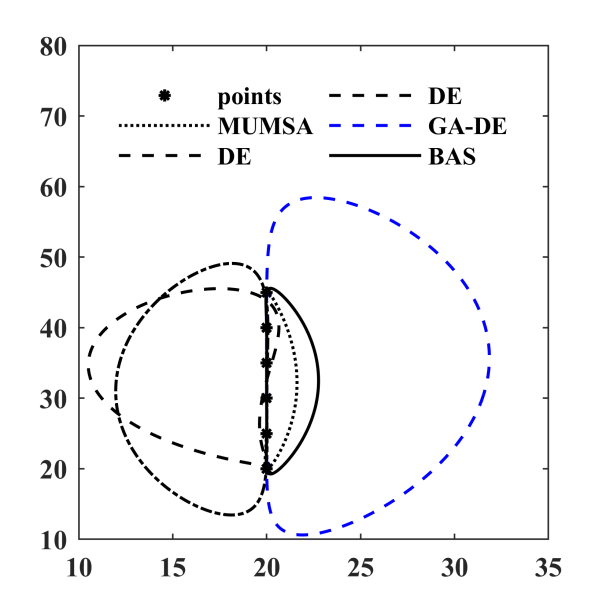
\includegraphics[width=0.5\linewidth]{img/case1png} 

}

\caption{各算法优化轨迹}\label{fig:case1png}
\end{figure}

\begin{table}[t]

\caption{\label{tab:case1table}case1各算法结果对比}
\centering
\begin{tabular}{lccccc}
\toprule
  & MUMSA & GA & DE & GA.DE & BAS\\
\midrule
$r_1$ & 31.788264 & 28.771330 & 35.020740 & 13.2516000 & 19.4920810\\
$r_2$ & 8.204647 & 5.000000 & 6.404196 & 5.9407800 & 6.2644716\\
$r_3$ & 24.932131 & 35.365480 & 31.607220 & 58.3118000 & 20.1001631\\
$r_4$ & 31.385926 & 59.136810 & 50.599490 & 53.7207000 & 19.0219161\\
$r_p$ & 37.108246 & 14.850370 & 46.461261 & 61.3011560 & 39.8538048\\
\addlinespace
$\theta_p$ & 0.398977 & 1.570796 & 1.106544 & -1.3002600 & 0.3679660\\
$\theta_0$ & 4.015959 & 5.287474 & 0.000000 & 0.1960760 & 4.4245619\\
$x_0$ & -6.366519 & 29.913290 & 60.000000 & -35.3621000 & -13.0300715\\
$y_0$ & 56.836760 & 32.602280 & 18.077910 & 36.7704000 & 51.1796666\\
$\theta_2^1$ & 1.366547 & 6.283185 & 6.283185 & 1.6601500 & 5.9699819\\
\addlinespace
$\theta_2^2$ & 2.330773 & 0.318205 & 0.264935 & 2.0468400 & 0.4554995\\
$\theta_2^3$ & 2.871039 & 0.638520 & 0.500377 & 2.4281100 & 1.0202707\\
$\theta_2^4$ & 3.394591 & 0.979950 & 0.735321 & 2.8090100 & 1.5550696\\
$\theta_2^5$ & 3.970960 & 1.412732 & 0.996529 & 3.1900900 & 2.1117409\\
$\theta_2^6$ & 4.963490 & 2.076254 & 1.333549 & 3.5737900 & 2.8839248\\
\addlinespace
$Error$ & 0.002057 & 1.101697 & 0.122738 & 0.0000172 & 0.0000124\\
\bottomrule
\end{tabular}
\end{table}

\subsection{Case2 有规定时间的轨迹生成(with prescribed
timing)}\label{case2-with-prescribed-timing}

本案例四杆机构的路径为5个没有对齐的点(规定时间)。通过式\eqref{eq:optim4bars}计算得到误差。

设计参数为:

\[
X = [r_1,r_2,r_3,r_4,r_p,\theta_p]
\] 目标点坐标:

\begin{align}
&\{C_d^i\} = \{(3,3),(2.759,3.363),(2.759,3.363),(1.890,3.862),(1.355,3.943)\} \notag \\
&\{\theta_2^1,\theta_2^2,\theta_2^3,\theta_2^4,\theta_2^5\}=\{\pi/6,\pi/4,\pi/3,5\pi/12,\pi/2\} \notag \\
\end{align}

参数约束:

\[
r_1,r_2,r_3,r_4\in[0,5]\quad r_p\in[-5,5]\quad \theta_p\in[0,2\pi]
\]

算法参数为
\(d_0 = 0.10,\delta_0=0.05,c_1=0.9998,c_2=0.5,q=40,T_{max}=10000\),动画结果如图\ref{fig:case2gif}。

\url{img/case2.gif}

与其他算法对比结果如图\ref{fig:case2png}和表\ref{tab:case2table}。

\begin{figure}

{\centering 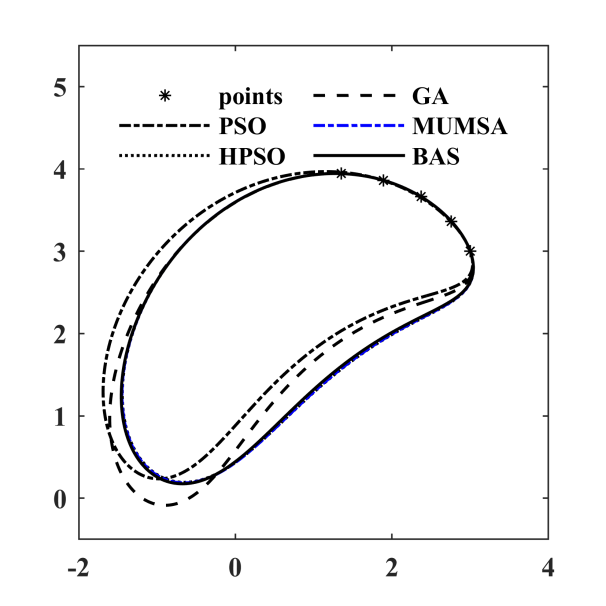
\includegraphics[width=0.5\linewidth]{img/case2png} 

}

\caption{各算法优化轨迹}\label{fig:case2png}
\end{figure}

\begin{table}[t]

\caption{\label{tab:case2table}case2各算法结果对比}
\centering
\begin{tabular}{lccccc}
\toprule
  & PSO & HPSO & GA & MUMSA & BAS\\
\midrule
$r_1$ & 3.0576200 & 3.7877200 & 3.0630424 & 3.7732686 & 3.7135255\\
$r_2$ & 1.8618400 & 1.9984200 & 1.9959624 & 2.0000040 & 1.9978745\\
$r_3$ & 3.8459100 & 4.1331300 & 3.3058230 & 4.1169710 & 4.0469527\\
$r_4$ & 2.9706300 & 2.7451300 & 2.5247060 & 2.7461567 & 2.7192391\\
$r_p$ & 2.4968270 & 2.3697220 & 2.3721479 & 2.3684374 & 2.3702974\\
\addlinespace
$\theta_p$ & 0.7243557 & 0.7841479 & 0.8044176 & 0.7831567 & 0.7865371\\
$Error$ & 0.0005860 & 0.0009860 & 0.0000018 & 0.0000018 & 0.0000007\\
\bottomrule
\end{tabular}
\end{table}

\subsection{Case3 规定时间内路径生成(Path generation with prescribed
timing)}\label{case3-path-generation-with-prescribed-timing}

本案例四杆机构需要在规定时间通过一个闭环。通过式\eqref{eq:optim4bars}计算得到误差。

设计参数为:

\[
X = [r_1,r_2,r_3,r_4,r_p,\theta_p,\theta_0,x_0,y_0,\theta_2^1,\cdots,\theta_2^6]
\]

目标点坐标:

\begin{align}
\{C_d^i\} = \{&(0.5,1.1),(0.4,1.1),(0.3,1.1),(0.2,1.0),(0.1,0.9),(0.05,0.75), \notag \\
&(0.02,0.6),(0,0.5),(0,0.4),(0.03,0.3),(0.1,0.25),(0.15,0.2), \notag\\
&(0.2,0.3),(0.3,0.4),(0.4,0.5),(0.5,0.7),(0.6,0.9),(0.6,1.0)\} \notag\\
\{\theta_2^i\}=\{&\theta_2^1,\theta_2^1+20\cdot i/\pi\},\quad i = 1,\cdots,17 \notag \\
\end{align}

参数约束:

\[
r_1,r_2,r_3,r_4\in[0,5]\quad r_p,x_0,y_0\in[-5,5]\quad \theta_0,\theta_2^1,\theta_p\in[0,2\pi]
\]

算法参数为
\(d_0 = 0.10,\delta_0=0.05,c_1=0.9998,c_2=0.5,q=8,T_{max}=50000\),动画结果如图\ref{fig:case3gif}。

\url{img/case3.gif}

与其他算法对比结果如图\ref{fig:case3png}和表\ref{tab:case3table}。

\begin{figure}

{\centering 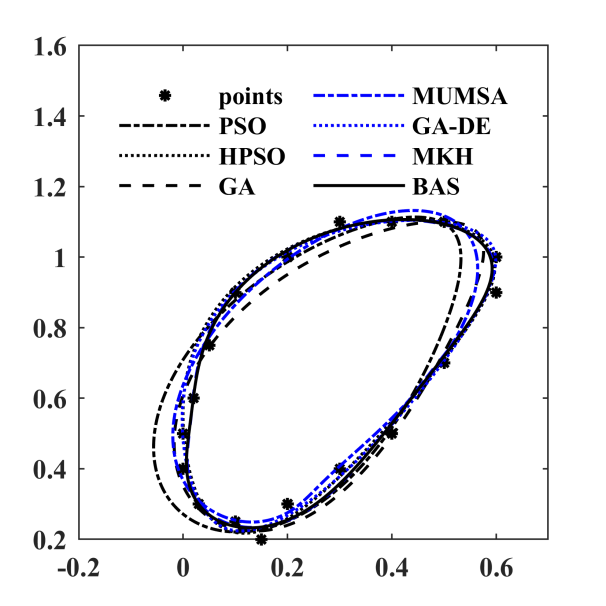
\includegraphics[width=0.5\linewidth]{img/case3png} 

}

\caption{各算法优化轨迹}\label{fig:case3png}
\end{figure}

\begin{table}[t]

\caption{\label{tab:case3table}case3各算法结果对比}
\centering
\begin{tabular}{lccccccc}
\toprule
  & PSO & HPSO & GA & MUMSA & GA.DE & MKH & BAS\\
\midrule
$r_1$ & 2.9261 & 2.8500 & 3.0579 & 4.4538 & 47.4379 & 1.0043 & 1.0542\\
$r_2$ & 0.4877 & 0.3700 & 0.2378 & 0.2971 & 0.3248 & 0.4218 & 0.4239\\
$r_3$ & 2.9099 & 2.9048 & 4.8290 & 3.9131 & 0.4729 & 0.8782 & 0.9146\\
$r_4$ & 2.1503 & 0.5000 & 2.0565 & 0.8494 & 47.3093 & 0.5801 & 0.5989\\
$r_p$ & 1.4939 & 1.9737 & 2.0035 & 2.6520 & 0.3413 & 0.5234 & 0.5450\\
\addlinespace
$\theta_p$ & -0.3325 & 1.0274 & 1.1779 & 2.4647 & -1.2154 & 0.8148 & 0.8227\\
$\theta_0$ & 0.7190 & 0.7600 & 1.0022 & 2.7387 & 3.3203 & 0.2929 & 0.2850\\
$x_0$ & -0.3846 & 0.9400 & 1.7768 & -1.3092 & 0.5270 & 0.2689 & 0.2677\\
$y_0$ & -0.6752 & -1.1712 & -0.6420 & 2.8070 & 0.7239 & 0.1772 & 0.1544\\
$\theta_2^1$ & 0.2159 & 0.5134 & 0.2262 & 4.8535 & 3.5123 & 0.8860 & 1.1764\\
\addlinespace
$Error$ & 0.0492 & 0.0111 & 0.0337 & 0.0196 & 0.0109 & 0.0091 & 0.0090\\
\bottomrule
\end{tabular}
\end{table}

\subsection{Case4 规定时间路径生成问题}\label{case4-}

第四个案例同样是一个规定时间的路径生成问题。六个优化点由一个\texttt{semi-archer}弧构成,问题定义如下。

设计参数为:

\[
X = [r_1,r_2,r_3,r_4,r_p,\theta_p,\theta_0,x_0,y_0]
\]

目标点坐标:

\begin{align}
&\{C_d^i\} = \{(0,0),(1.9098,5.8779),(6.60989.5106),(13.09,9.5106),(18.09,5.8779),(20,0)\} \notag \\
&\{\theta_2^1,\theta_2^2,\theta_2^3,\theta_2^4,\theta_2^5\}=\{\pi/6,\pi/3,\pi/2,2\pi/3,5\pi/6,\pi\} \notag \\
\end{align}

参数约束:

\[
r_1,r_2,r_3,r_4\in[0,50]\quad r_p,x_0,y_0\in[-50,50]\quad \theta_0,\theta_p\in[0,2\pi]
\]

算法参数为
\(d_0 = 0.10,\delta_0=0.05,c_1=0.9997,c_2=0.5,q=40,T_{max}=30000\),动画结果如图\ref{fig:case4gif}。

\url{img/case4.gif}

与其他算法对比结果如图\ref{fig:case4png}和表\ref{tab:case4table}。

\begin{figure}

{\centering 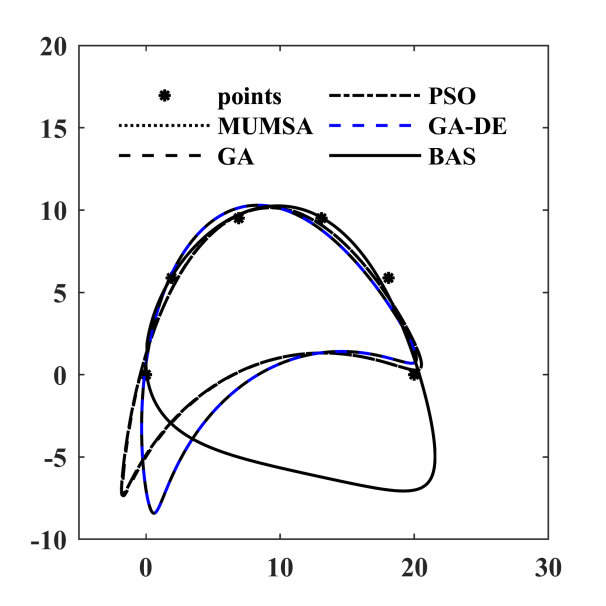
\includegraphics[width=0.5\linewidth]{img/case4png} 

}

\caption{各算法优化轨迹}\label{fig:case4png}
\end{figure}

\begin{table}[t]

\caption{\label{tab:case4table}case4各算法结果对比}
\centering
\begin{tabular}{lccccc}
\toprule
  & MUMSA & GA & PSO & GA.DE & BAS\\
\midrule
$r_1$ & 50.0000000 & 50.0000000 & 50.0000000 & 50.000000 & 47.2345017\\
$r_2$ & 5.0000000 & 5.0000000 & 5.0000000 & 5.000000 & 8.8473992\\
$r_3$ & 7.0310470 & 6.9700900 & 7.0310200 & 5.905343 & 25.0474709\\
$r_4$ & 48.1341830 & 48.1993000 & 48.1342000 & 50.000000 & 50.0000000\\
$r_p$ & 21.3533558 & 21.2191204 & 21.3532819 & 18.819312 & 50.0000000\\
\addlinespace
$\theta_p$ & 0.6517294 & 0.6380060 & 0.6517238 & 0.000000 & 5.7107187\\
$\theta_0$ & 0.0428247 & 0.0508453 & 0.0428286 & 0.463633 & 0.8225945\\
$x_0$ & 12.1974940 & 12.2377000 & 12.1975000 & 14.373772 & 16.5531171\\
$y_0$ & -15.9982030 & -15.8332000 & -15.9981000 & -12.444295 & -48.1473786\\
$Error$ & 2.5803500 & 2.5828600 & 2.5803600 & 2.349649 & 0.7863680\\
\bottomrule
\end{tabular}
\end{table}

\subsection{Case5 规定时间内路径生成问题}\label{case5-}

这个例子是一个椭圆路径生成问题,没有规定的时间,其中轨迹是由10个点定义的。问题定义如下。

设计参数为:

\[
X = [r_1,r_2,r_3,r_4,r_p,\theta_p,\theta_0,x_0,y_0,\theta_2^1,\cdots,\theta_2^{10}]
\]

目标点坐标:

\begin{align}
\{C_d^i\} = \{&(20,10),(17.66,15.142),(11.736,17.878),(5,16.928),(0.60307,12.736), \notag \\
&(0.60307,7.2638),(5,3.0718),(11.736,2.1215),(17.66,4.8577),(20,0)\}\notag\\
\end{align}

参数约束:

\[
r_1,r_2,r_3,r_4\in[0,80]\quad r_p,x_0,y_0\in[-80,80]\quad \theta_0,\theta_2^1,\cdots,\theta_2^{10},\theta_p\in[0,2\pi]
\]

算法参数为
\(d_0 = 0.10,\delta_0=0.05,c_1=0.9998,c_2=0.5,q=40,T_{max}=40000\),动画结果如图\ref{fig:case5gif}。

\url{img/case5.gif}

与其他算法对比结果如图\ref{fig:case5png}和表\ref{tab:case5table}。

\begin{figure}

{\centering 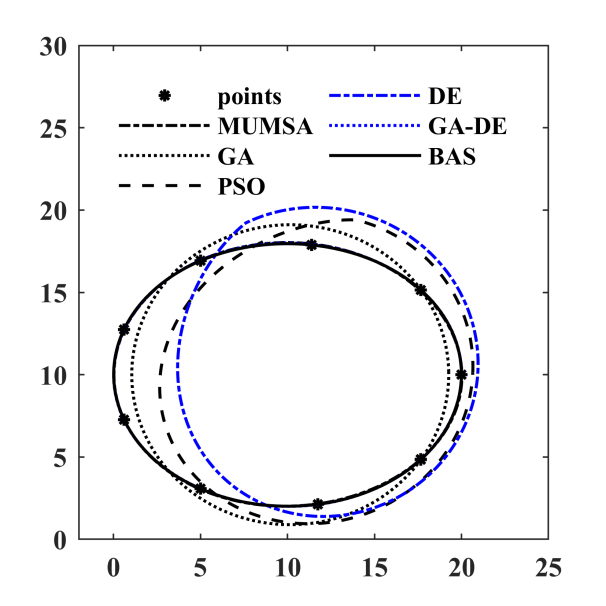
\includegraphics[width=0.5\linewidth]{img/case5png} 

}

\caption{各算法优化轨迹}\label{fig:case5png}
\end{figure}

\begin{table}[t]

\caption{\label{tab:case5table}case5各算法结果对比}
\centering
\begin{tabular}{lcccccc}
\toprule
  & MUMSA & GA & PSO & DE & GA.DE & BAS\\
\midrule
$r_1$ & 79.5160680 & 79.981513 & 52.535162 & 54.360893 & 80.0000000 & 71.8681225\\
$r_2$ & 9.7239730 & 9.109993 & 8.687886 & 8.683351 & 8.4203200 & 9.2618623\\
$r_3$ & 45.8425240 & 72.936511 & 36.155078 & 34.318634 & 51.3426000 & 44.4542963\\
$r_4$ & 51.4384800 & 80.000000 & 80.000000 & 79.996171 & 42.4532000 & 43.0533508\\
$r_p$ & 8.7289390 & 0.000000 & 1.481055 & 1.465250 & 10.6530404 & 8.7820722\\
\addlinespace
$\theta_p$ & -0.3452264 & 0.000000 & 1.570796 & 1.570669 & 2.6465448 & 1.6362575\\
$\theta_0$ & 5.5969445 & 0.026149 & 1.403504 & 2.129650 & 4.2817700 & 1.6011655\\
$x_0$ & 2.0211090 & 10.155966 & 11.002124 & 10.954397 & 5.5337200 & 16.7540360\\
$y_0$ & 13.2165878 & 10.000000 & 11.095585 & 11.074534 & 0.4771830 & 15.2986682\\
$\theta_2^1$ & 0.6376873 & 6.283185 & 6.282619 & 6.283185 & 2.0935000 & 0.1258416\\
\addlinespace
$\theta_2^2$ & 1.3255329 & 0.600745 & 0.615302 & 0.616731 & 2.8129100 & 0.8167208\\
$\theta_2^3$ & 2.0080339 & 1.372812 & 1.305421 & 1.310254 & 3.5160500 & 1.5351326\\
$\theta_2^4$ & 2.6955659 & 2.210575 & 2.188053 & 2.193570 & 4.2063800 & 2.1811489\\
$\theta_2^5$ & 3.3845794 & 2.862639 & 2.913049 & 2.917170 & 4.8905100 & 2.8753839\\
$\theta_2^6$ & 4.0829376 & 3.420547 & 3.499313 & 3.490746 & 5.5739800 & 3.5728072\\
\addlinespace
$\theta_2^7$ & 4.7984548 & 4.072611 & 4.125586 & 4.132017 & 6.2645800 & 4.2854058\\
$\theta_2^8$ & 5.5117056 & 4.910373 & 4.919977 & 4.922075 & 0.6761980 & 5.0016208\\
$\theta_2^9$ & 6.2127919 & 5.682440 & 5.685021 & 5.695372 & 1.3830700 & 5.7133417\\
$\theta_2^{10}$ & 0.6371866 & 6.283185 & 6.282323 & 6.282970 & 2.0934800 & 0.1258290\\
$Error$ & 0.0047000 & 2.281273 & 1.971004 & 1.952326 & 0.0006022 & 0.0004252\\
\bottomrule
\end{tabular}
\end{table}

\subsection{Case6 六杆机构路径生成}\label{case6-}

这个案例我也看不懂。大概意思是,六杆问题,在规定时间内让轨迹耦合目标点,并且\texttt{output\ link}在停顿位置(\texttt{dwell\ portion}?我翻译不下去了\ldots{}\ldots{})保持在一个精确的角度。大家看底下的原文靠谱一点。

\begin{quote}
``This case is a path and function combined synthesis problem with
prescribed timing in which the coupler of six-bar mechanism has to the
precision points and its output link has to maintain an accuracy angle
in the dwell portion.''

\begin{flushright}--- Xiaojuan Mo\end{flushright}
\end{quote}

设计参数为:

\[
X = [r_1,r_2,r_3,r_4,r_5,r_6,r_p,\theta_p,r_1',\theta_0,\theta_0',x_0,y_0,\theta_2^1] 
\]

目标点坐标:

\begin{align}
\{C_d^i\} = \{&(-0.5424,2.3708),(0.2202,2.9871),(0.9761,3.4633), \notag \\
&(1.0618,36380),(0.8835,3.7226),(0.5629,3.7156),\notag \\
&(0.1744,3.6128),(-0.2338,3.4206),(-0.6315,3.1536), \notag \\
&(-1.0,2.8284),(-1.3251,2.4600),(-1.5922,2.0622), \notag \\
&(-1.7844,1.6539),(-1.8872,1.2654),(-1.8942,0.9448), \notag \\
&(-1.8096,0.7665),(-1.6349,0.8522),(-1.1587,1.6081)\} \notag \\
\{\theta_2^i\} = \{&0,15,40,60,80,100,120,140,160,180,\notag \\
& 200, 220,240,260,280,300,320,345\} \notag \\
& \rightarrow \theta_2^i = \theta_2 + \delta_2^i \notag \\
\end{align}

在停顿位置处的输入输出角度的关联如下:

\begin{align}
&\theta_2^i = \theta_2^1+\{160,180,200,220\}\rightarrow \theta_6^i=210 \notag \\
&\theta_2^i=\theta_2^1+\{345,0,15\} \rightarrow \theta_6^i = 225 \notag \\
\end{align}

\begin{quote}
注意,上述涉及到角度的数值单位均为deg,而非弧度。
\end{quote}

算法参数为
\(d_0 = 0.05,\delta_0=0.025,c_1=0.9999,c_2=0.5,q=10,T_{max}=50000\),动画结果如图\ref{fig:case6gif}。

\url{img/case6.gif}

与其他算法对比结果如图\ref{fig:case6png},
图\ref{fig:case6png2}和表\ref{tab:case6table}。

\begin{figure}

{\centering 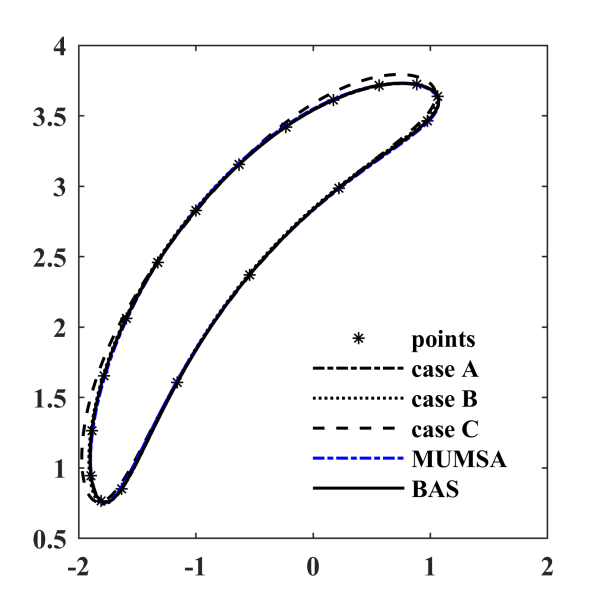
\includegraphics[width=0.5\linewidth]{img/case6png} 

}

\caption{各算法优化轨迹}\label{fig:case6png}
\end{figure}

\begin{figure}

{\centering 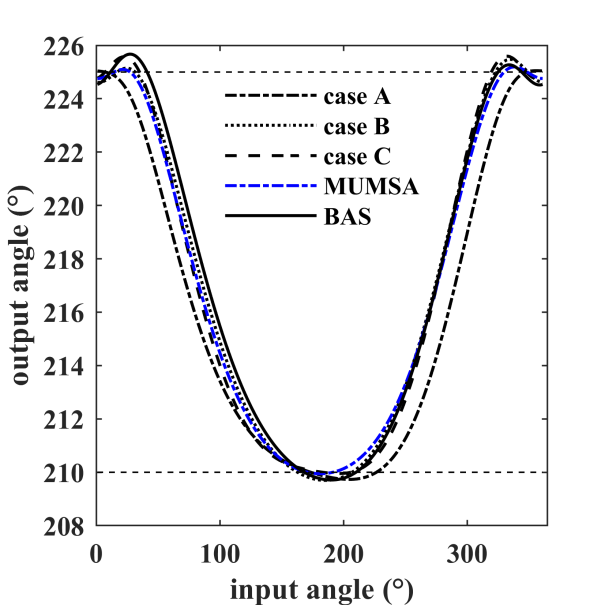
\includegraphics[width=0.5\linewidth]{img/case6png2} 

}

\caption{各算法优化角度}\label{fig:case6png2}
\end{figure}

\begin{table}[t]

\caption{\label{tab:case6table}case6各算法结果对比}
\centering
\begin{tabular}{lccccc}
\toprule
  & DE.A & DE.B & DE.C & MUMSA & BAS\\
\midrule
$r_1$ & 1.8145 & 1.8065 & 2.0926 & 1.713529 & 1.838058488\\
$r_2$ & 0.9911 & 0.9826 & 1.1464 & 0.92602 & 1.006097698\\
$r_3$ & 1.9995 & 2.0177 & 1.989 & 1.991373 & 1.997800646\\
$r_4$ & 2.0315 & 2.0009 & 1.9727 & 1.848672 & 2.008472163\\
$r_5$ & 4.3674 & 5.7769 & 6.6633 & 5.35498 & 6.106586728\\
\addlinespace
$r_6$ & 2.4924 & 2.5296 & 2.5517 & 2.54979 & 2.551492193\\
$r_p$ & 2.8174 & 2.8711 & 2.7178 & 2.975936132 & 2.815041279\\
$\theta_p$ & 0.7776 & 0.783712 & 0.845246 & 0.831651258 & 0.78386985\\
$\theta_0$ & 6.269879 & 0.011582 & 6.242260827 & 0.067677 & 6.277427755\\
$r_1'$ & 4.4158 & 5.2817 & 6.2907 & 4.87374 & 5.63828226\\
\addlinespace
$\theta_0'$ & 0.235595 & 0.0170309 & 6.18118303 & 0.0967027 & 6.257863894\\
$x_0$ & 0.0115 & 0.0415 & -0.2729 & 0.175257 & -0.013849346\\
$y_0$ & 0.0157 & -0.0377 & 0.0931 & -0.1187032 & 0.011591976\\
$\theta_2^1$ & 0.00052 & 0.003648 & -0.04062 & 6.222361 & 6.281768246\\
$Evaluations$ & 53310 & 93405 & 93405 & 93405 & 50000\\
\addlinespace
$Error$ & 0.000250876 & 0.005653158 & 0.03537533 & 0.0014 & 0.000195212659\\
\bottomrule
\end{tabular}
\end{table}

\subsection{Case7 无规定时间的路径生成}\label{case7-}

本案例为一个'8'型路径生成问题,轨迹由12个点规定。

设计参数为:

\[
X = [r_1,r_2,r_3,r_4,r_p,\theta_p,\theta_0,x_0,y_0,\theta_2^1,\cdots,\theta_2^{12}]
\]

目标点坐标:

\begin{align}
\{C_d^i\} = \{&(4.15,2.21),(4.50,2.18),(4.53,1.83),(4.13,1.68),(3.67,1.58),(2.96,1.33), \notag \\
&(2.67,1.06),(2.63,0.82),(2.92,0.81),(3.23,1.07),(3.49,1.45),(3.76,1.87)\}\notag\\
\end{align}

参数约束:

\begin{align}
&r_1\in[0,5]\quad r_2,r_3,r_4\in[0,10] \quad r_p\in[0,14],\notag \\
&x_0,y_0\in[-80,80]\quad \theta_0,\theta_2^1,\cdots,\theta_2^{12},\theta_p\in[0,2\pi] \notag \\
\end{align}

算法参数为
\(d_0 = 0.05,\delta_0=0.025,c_1=0.9995,c_2=0.5,q=40,T_{max}=20000\),动画结果如图\ref{fig:case7gif}。

\url{img/case7.gif}

与其他算法对比结果如图\ref{fig:case7png}和表\ref{tab:case7table}。

\begin{figure}

{\centering 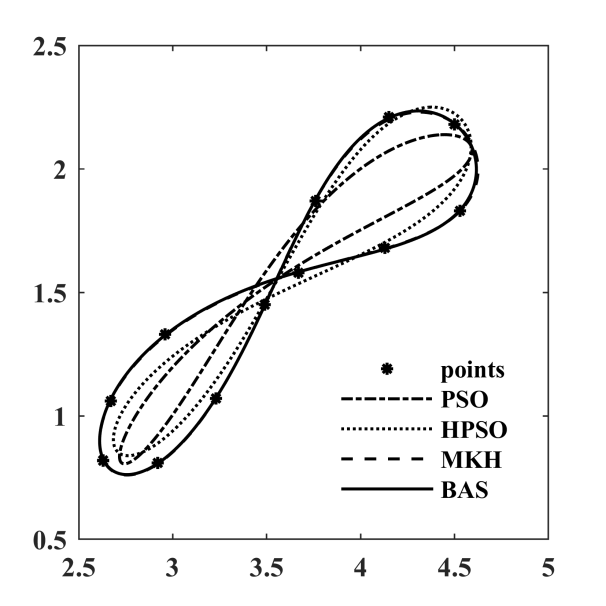
\includegraphics[width=0.5\linewidth]{img/case7png} 

}

\caption{各算法优化轨迹}\label{fig:case7png}
\end{figure}

\begin{table}[t]

\caption{\label{tab:case7table}case7各算法结果对比}
\centering
\begin{tabular}{lcccc}
\toprule
  & PSO & HPSO & MKH & BAS\\
\midrule
$r_1$ & 4.550300 & 4.535900 & 2.8764500 & 2.8162769\\
$r_2$ & 1.101300 & 1.113300 & 1.1464400 & 1.1382629\\
$r_3$ & 3.955800 & 14.738100 & 4.4077300 & 4.0509922\\
$r_4$ & 3.933000 & 16.801700 & 4.7571300 & 4.1957758\\
$r_p$ & 3.941572 & 3.941866 & 2.6665746 & 2.6682801\\
\addlinespace
$\theta_p$ & -0.539171 & -1.521104 & -1.1363513 & 5.1910788\\
$\theta_0$ & 0.000000 & 0.000000 & 0.1650200 & 0.2070603\\
$x_0$ & 0.000000 & 0.000000 & 1.1426500 & 1.1226995\\
$y_0$ & 0.000000 & 0.000000 & 0.4823700 & 0.5246662\\
$\theta_2^1$ & -0.201400 & -0.181600 & -0.3139900 & 6.1191060\\
\addlinespace
$Error$ & 0.171600 & 0.096400 & 0.0001597 & 0.0000994\\
\bottomrule
\end{tabular}
\end{table}

\subsection{Case8 无规定时间的路径生成}\label{case8-}

本案例为一个叶形路径生成问题(无规定时间),轨迹由25个点规定。

设计参数为:

\[
X = [r_1,r_2,r_3,r_4,r_p,\theta_p,\theta_0,x_0,y_0,\theta_2^1,\cdots,\theta_2^{25}]
\]

目标点坐标:

\begin{align}
\{C_d^i\} = \{&(7.03,5.99),(6.95,5.45),(6.77,5.03),(6.4,4.6),(5.91,4.03), \notag \\
&(5.43,3.56),(4.93,2.94),(4.67,2.6),(4.38,2.2),(4.04,1.67),\notag \\
&(3.76,1.22),(3.76,1.97),(3.76,2.78),(3.76,3.56),(3.76,4.34), \notag \\
&(3.76,4.91),(3.76,5.47),(3.8,5.98),(4.07,6.4),(4.53,6.75), \notag \\
&(5.07,6.85),(5.05,6.84),(5.89,6.83),(6.41,6.8),(6.92,6.58)\} \notag \\
\end{align}

参数约束:

\[
r_1,r_2,r_3,r_4\in[0,5]\quad r_p,x_0,y_0\in[-5,5] \quad \theta_0,\theta_2^1,\cdots,\theta_2^{25},\theta_p\in[0,2\pi]
\]

算法参数为
\(d_0 = 0.05,\delta_0=0.025,c_1=0.99975,c_2=0.5,q=40,T_{max}=50000\),动画结果如图\ref{fig:case8gif}。

\url{img/case8.gif}

与其他算法对比结果如图\ref{fig:case8png}和表\ref{tab:case8table}。

\begin{figure}

{\centering 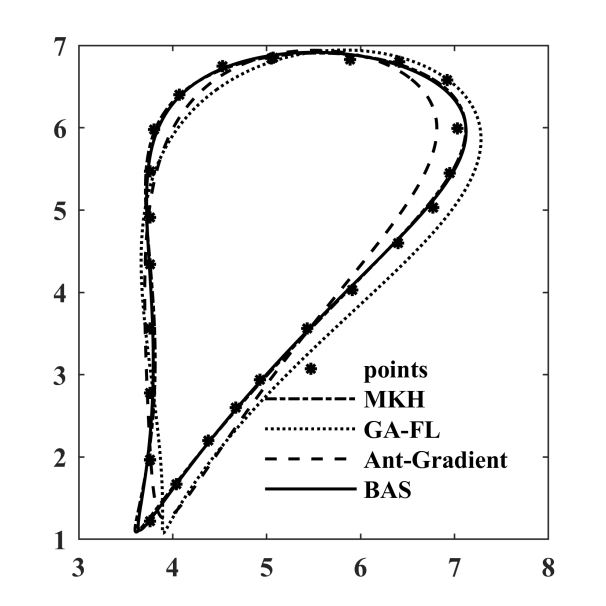
\includegraphics[width=0.5\linewidth]{img/case8png} 

}

\caption{各算法优化轨迹}\label{fig:case8png}
\end{figure}

\begin{table}[t]

\caption{\label{tab:case8table}case8各算法结果对比}
\centering
\begin{tabular}{lcccc}
\toprule
  & MKH & GA.FL & Ant.Gradient & BAS\\
\midrule
$r_1$ & 9.99432 & 9 & 13.08 & 9.6132193\\
$r_2$ & 1.93027 & 3.01 & 1.89 & 1.9459840\\
$r_3$ & 4.57242 & 8.8 & 8.41 & 4.9080817\\
$r_4$ & 7.36674 & 8.8 & 6.75 & 6.6768279\\
$r_p$ & 8.04254 & 11.0995 & 14.45 & 8.6409226\\
\addlinespace
$\theta_p$ & 0.187430 & -0.681 & 0.195 & 0.1694076\\
$\theta_0$ & -0.61763 & 0.489 & -0.3815 & 5.7260733\\
$x_0$ & -2.31301 & -2.4 & -8.77 & -2.9214626\\
$y_0$ & 2.86189 & -4 & 1.20 & 2.7190256\\
$\theta_2^1$ & * & * & * & 0.4529787\\
\addlinespace
$Error$ & 0.03916 & 0.9022 & 0.5504 & 0.0397777\\
\bottomrule
\end{tabular}
\end{table}

\chapter{BAS案例二:龙门起重机运动控制}\label{examples2}

\begin{quote}
由群友李晓晓同学提供案例。
\end{quote}

\section{问题背景}

龙门起重机(gantry
crane),如图\ref{fig:gc}所示,是水平桥架设置在两条支腿上构成门架形状的一种桥架型起重机。起重小车trolley在桥架上运行,利用绳索(cable)一类的柔性体连接负载(load)。在负载的输送过程中,load的摆动问题一直是影响吊车装运效率提高的一大难题。

\begin{figure}

{\centering 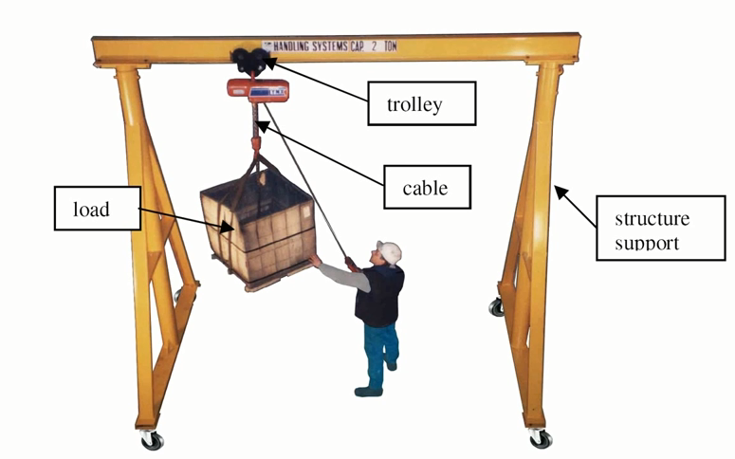
\includegraphics[width=0.7\linewidth]{img/gc} 

}

\caption{龙门起重机示意}\label{fig:gc}
\end{figure}

模型可以简化为图\ref{fig:gc2}。重物通过绳索与小车相连,小车在外力的作用下水平运动,小车质量为M(kg),重物的质量为m(kg),绳索的长度为r(m),\(\theta\)为摆角,x表示水平方向上的位移。

\begin{figure}

{\centering 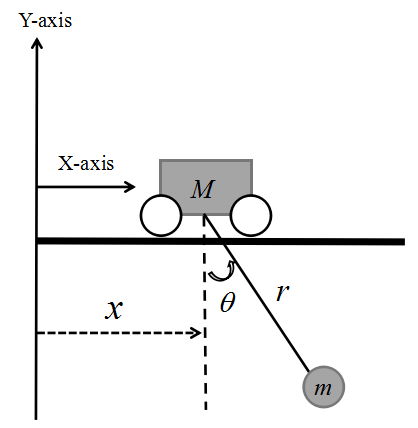
\includegraphics[width=0.6\linewidth]{img/gc2} 

}

\caption{龙门起重机模型}\label{fig:gc2}
\end{figure}

\section{优化问题抽象}

优化的变量为\texttt{bang-coast-bang}控制中,\(x = [tp_1,tp_2,tf]^T\),两个给予脉冲加速度激励的时段以及全部的作业时间,以此来使得负载的摆角(优化目标)最小。

取小车的位置x,摆角\(\theta\)作为系统的广义坐标系。小车和负载在t时刻的位置坐标如式\eqref{eq:loadposition}所示。

\begin{equation}
\begin{cases} 
x_M(t)&=\quad x(t)\\ 
y_M(t)&=\quad 0 \\
x_m(t)&=\quad x(t)+rsin\theta(t)\\
t_m(t)&=\quad -rco\theta(t)
\end{cases}
\label{eq:loadposition}
\end{equation}

因此,对\(t\)求导,得到小车和负载的速度分量如式\eqref{eq:speedp}所示。

\begin{equation}
\begin{cases} 
\dot{x}_M(t) &=\quad \dot{x}_t\\
\dot{y}_M(t) &=\quad 0\\
\dot{x}_m(t) &=\quad \dot{x}(t)+r\dot{\theta}(t)cos\theta(t)\\
\dot{y}_m(t) &=\quad r\dot{\theta}(t)sin\theta(t)
\end{cases}
\label{eq:speedp}
\end{equation}

系统动能如式\eqref{eq:kineticenergy}:

\begin{equation}
\begin{split}
T  = &\frac{1}{2}MV_M^2(t) + \frac{1}{2}mV_m^2(t) \\
=&\frac{1}{2}M(\dot{x}_M^2(t)+\dot{y}_M^2(t))+\frac{1}{2}m(\dot{x}_m^2(t)+\dot{y}_m^2(t))\\
=&\frac{1}{2}M\dot{x}_M^2(t) + \frac{1}{2}m\dot{x}_m^2(t) + \\
&\frac{1}{2}mr^2\dot{\theta}^2(t) + mr\dot{x}(t)\dot{\theta}(t)cos\theta(t)
\end{split}
\label{eq:kineticenergy}
\end{equation}

势能如式\eqref{eq:potentialenergy}:

\begin{equation}
P = -mgrcos\theta(t)
\label{eq:potentialenergy}
\end{equation}

通过式\eqref{eq:potentialenergy}和式\eqref{eq:kineticenergy},我们可以得到拉格朗日方程,即\(L = T -P\)。根据欧拉-拉格朗日方程(Euler-Lagrangian
equation),龙门起重机的动力学模型如式\eqref{eq:EL}所示。

\begin{equation}
\frac{d}{dt}[\frac{\partial{L}}{\partial{\dot{q_k}}}] - \frac{\partial{L}}{\partial{q_k}}=Q_k, \quad k=1,\cdots,n
\label{eq:EL}
\end{equation}

其中,\(n\)表示系统的自由度,\(\{q_1,\cdots,q_n\}\)表示广义坐标集合,\(\{Q_1,\cdots,Q_n\}\)表示广义的驱动力(对应于各自的广义坐标)。把摆角作为广义坐标,可以得到式\eqref{eq:thetaEL1}。

\begin{equation}
\frac{d}{dt}[\frac{\partial{L}}{\partial{\dot{\theta}}}] - \frac{\partial{L}}{\partial{\theta}}=0
\label{eq:thetaEL1}
\end{equation}

第一项为\(mr^2\ddot{\theta}(t)+mr\ddot{x}(t)cos\theta(t)\),第二项为\(-mgrsin\theta(t)\),代入式\eqref{eq:thetaEL1}中可以得到\(\theta\)的求解方程,即式\eqref{eq:thetaEL2}。

\begin{equation}
\ddot{\theta}(t)=-\frac{\ddot{x}(t)cos\theta(t)+gsin\theta(t)}{r}
\label{eq:thetaEL2}
\end{equation}

通过求解该方程,我们可以得到我们的优化目标。

\section{优化理论}\label{-1}

优化理论为二阶BAS算法。李晓晓同学给出的参数是,\(w_0 = 0.7\),
\(w_1 = 0.2\)。当然,文档中对于不同的目标函数可能有不同的调参结果,大家可以自行调试。

\section{优化结果}\label{-1}

\begin{table}[t]

\caption{\label{tab:example2parms}实验参数取值}
\centering
\begin{tabular}{ccc}
\toprule
Parameter & Description & Values\\
\midrule
$c$ & Constant & 5\\
$\lambda$ & Step length ratio & 0.95\\
$\gamma$ & Penalty coefficient & $10^{50}$\\
$n$ & Number of iterations & 1000\\
$r$ & Height of crane & 20(m)\\
\addlinespace
$h$ & Load displacement & 40(m)\\
\bottomrule
\end{tabular}
\end{table}

\begin{table}[t]

\caption{\label{tab:example2result}优化结果对比}
\centering
\begin{tabular}{ccc}
\toprule
Variables & fmincon & BAS\\
\midrule
$tp_1$ & 8.9624000 & 6.9082000\\
$tp_2$ & 8.9803000 & 6.9741000\\
$tf$ & 19.8346000 & 15.8866000\\
$f$ & 0.0029586 & 0.0001415\\
\bottomrule
\end{tabular}
\end{table}

从表\ref{tab:example2result}中可以看到,BAS能够让起重机小车在7秒内加速到最大速度,在16秒内就能到达终点并消除摆角。动图\ref{fig:example2fminconbob}至\ref{fig:example2bastrace}分别为采用\texttt{fmincon}和\texttt{BAS}做优化的结果,可以让我们有更为直观的认识。

\url{img/fminconbob.gif}

\url{img/BASbob.gif}

\url{img/fmincontrace.gif}

\url{img/BAStrace.gif}

\begin{figure}

{\centering 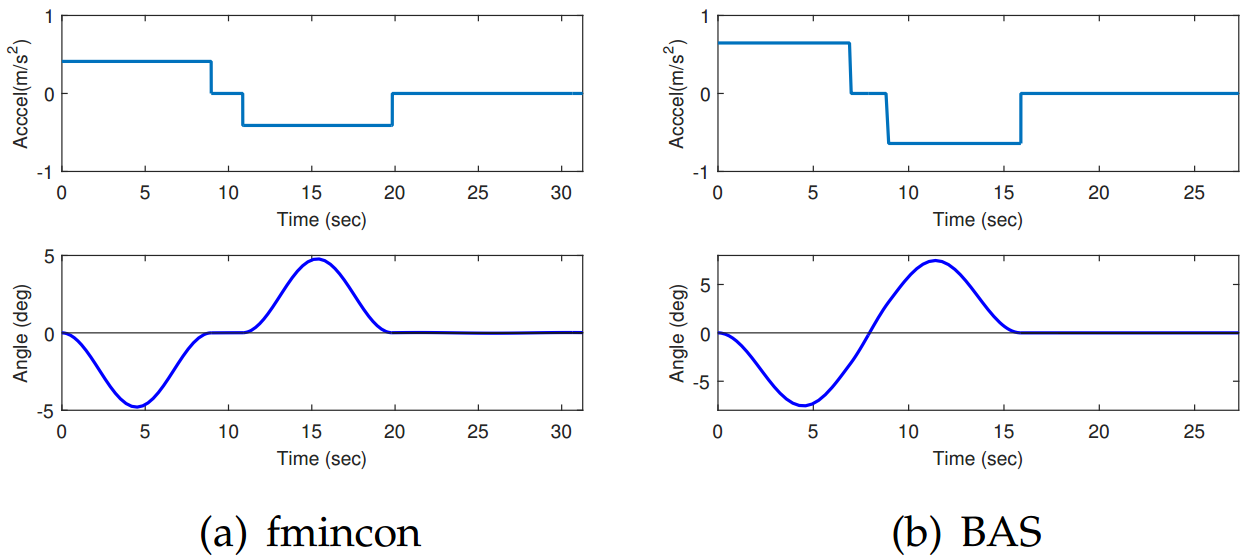
\includegraphics[width=0.7\linewidth]{img/ex2_1} 

}

\caption{起重小车加速度曲线}\label{fig:ex2accel}
\end{figure}

\begin{figure}

{\centering 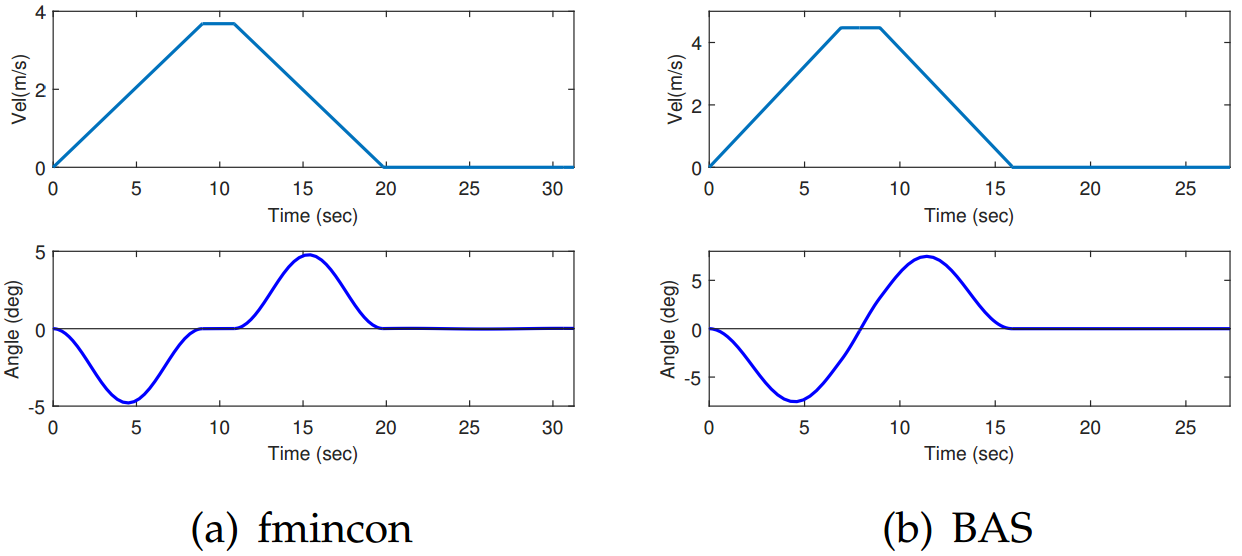
\includegraphics[width=0.7\linewidth]{img/ex2_2} 

}

\caption{起重小车速度曲线}\label{fig:ex2velocity}
\end{figure}

\begin{figure}

{\centering 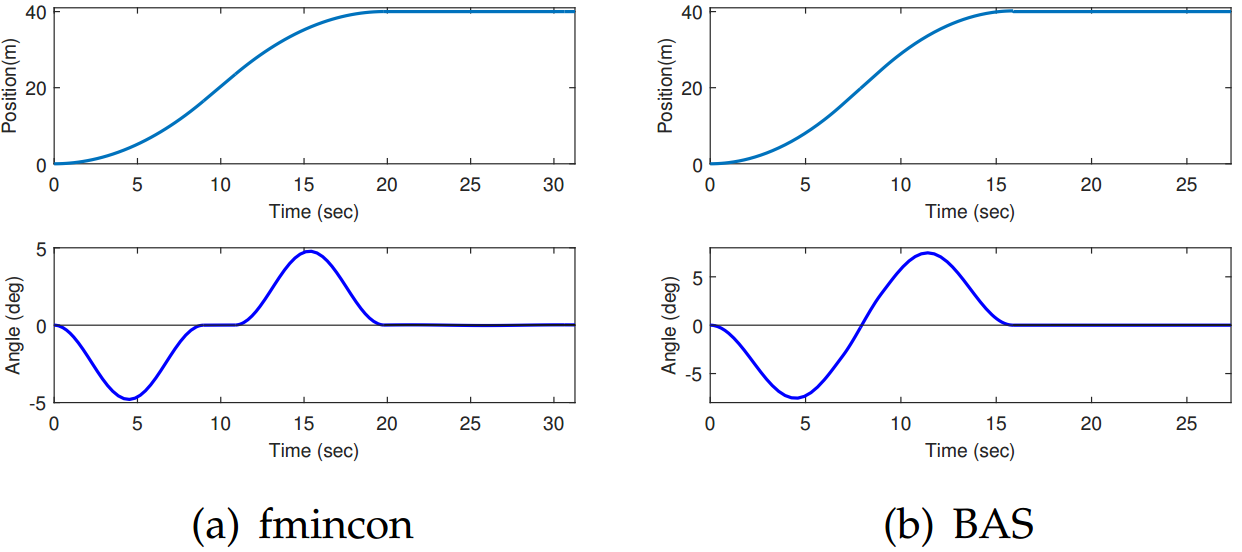
\includegraphics[width=0.7\linewidth]{img/ex2_3} 

}

\caption{起重小车位置曲线}\label{fig:ex2position}
\end{figure}

\chapter{Python接口}\label{python}

项目地址 \url{https://github.com/whhxp/Platypus} 。由吴会欢同学fork
\href{https://github.com/Project-Platypus/Platypus}{Platypus}项目后,修改而来。

\begin{quote}
文档内容由吴会欢同学提供。
\end{quote}

\section{安装方式}

在线安装

\begin{Shaded}
\begin{Highlighting}[]
\NormalTok{pip install git}\OperatorTok{+}\NormalTok{https:}\OperatorTok{//}\NormalTok{github.com}\OperatorTok{/}\NormalTok{whhxp}\OperatorTok{/}\NormalTok{Platypus.git}
\end{Highlighting}
\end{Shaded}

还可以本地安装。

利用git 将项目克隆到本地,然后目录改为文件目录后,进行安装。

\begin{Shaded}
\begin{Highlighting}[]
\NormalTok{git clone https:}\OperatorTok{//}\NormalTok{github.com}\OperatorTok{/}\NormalTok{whhxp}\OperatorTok{/}\NormalTok{Platypus.git}
\NormalTok{cd Platypus}
\NormalTok{python setup.py install}
\end{Highlighting}
\end{Shaded}

\section{使用}

Platypus是一个多目标优化库。这里我们将通过一个例子来简单介绍如何在Platypus中使用BAS。首先我们需要导入需要使用的函数

\begin{Shaded}
\begin{Highlighting}[]
\ImportTok{from}\NormalTok{ platypus }\ImportTok{import}\NormalTok{ Problem, Real}
\ImportTok{from}\NormalTok{ platypus.algorithms.bas }\ImportTok{import}\NormalTok{ BAS}
\ImportTok{from}\NormalTok{ math }\ImportTok{import}\NormalTok{ sin, pi, cos, exp, sqrt}
\end{Highlighting}
\end{Shaded}

下一步,我们需要创建问题,这里我找了三个问题作为例子。

第一个问题是Goldstein and Price problem。

\begin{figure}

{\centering 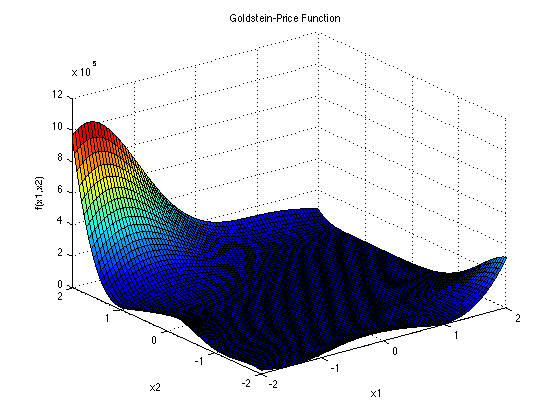
\includegraphics[width=0.7\linewidth]{img/python1} 

}

\caption{Goldstein-Price problem}\label{fig:python1}
\end{figure}

\begin{equation}
\begin{split}
f({x})=& [1+(x_1+x_2+1)^2(19-14x_1+3x_1^2-14x_2\notag \\
& +6x_1x_2+3x_2^2)][30+(2x_1-3X_2)^2(18-32x_1\notag  \\
& +12x_1^2+48x_2-36x_1x_2+27x_2^2)]\notag
\end{split}
\end{equation}

这个函数通常在正方形区间 \(x_i \in[-2,2]\)中进行评估,其中\(i = 1,2\).
全局最小值在\(x^*=(0,-1)\)处,为\(f(x^*)=3\)。

\begin{Shaded}
\begin{Highlighting}[]
\KeywordTok{class}\NormalTok{ gold(Problem):}
    \KeywordTok{def} \FunctionTok{__init__}\NormalTok{(}\VariableTok{self}\NormalTok{):}
        \BuiltInTok{super}\NormalTok{(gold, }\VariableTok{self}\NormalTok{).}\FunctionTok{__init__}\NormalTok{(nvars}\OperatorTok{=}\DecValTok{2}\NormalTok{, nobjs}\OperatorTok{=}\DecValTok{1}\NormalTok{)}
        \VariableTok{self}\NormalTok{.types[:] }\OperatorTok{=}\NormalTok{ [Real(}\OperatorTok{-}\DecValTok{2}\NormalTok{, }\DecValTok{2}\NormalTok{), Real(}\OperatorTok{-}\DecValTok{2}\NormalTok{, }\DecValTok{2}\NormalTok{)]}

    \KeywordTok{def}\NormalTok{ evaluate(}\VariableTok{self}\NormalTok{, solution):}
        \BuiltInTok{vars} \OperatorTok{=}\NormalTok{ solution.variables[:]}
\NormalTok{        x1 }\OperatorTok{=} \BuiltInTok{vars}\NormalTok{[}\DecValTok{0}\NormalTok{]}
\NormalTok{        x2 }\OperatorTok{=} \BuiltInTok{vars}\NormalTok{[}\DecValTok{1}\NormalTok{]}
\NormalTok{        fact1a }\OperatorTok{=}\NormalTok{ (x1 }\OperatorTok{+}\NormalTok{ x2 }\OperatorTok{+} \DecValTok{1}\NormalTok{) }\OperatorTok{**} \DecValTok{2}
\NormalTok{        fact1b }\OperatorTok{=} \DecValTok{19} \OperatorTok{-} \DecValTok{14} \OperatorTok{*}\NormalTok{ x1 }\OperatorTok{+} \DecValTok{3} \OperatorTok{*}\NormalTok{ x1 }\OperatorTok{**} \DecValTok{2} \OperatorTok{-} \DecValTok{14} \OperatorTok{*}\NormalTok{ x2 }\OperatorTok{+} \DecValTok{6} \OperatorTok{*}\NormalTok{ x1 }\OperatorTok{*}\NormalTok{ x2 }\OperatorTok{+} \DecValTok{3} \OperatorTok{*}\NormalTok{ x2 }\OperatorTok{**} \DecValTok{2}
\NormalTok{        fact1 }\OperatorTok{=} \DecValTok{1} \OperatorTok{+}\NormalTok{ fact1a }\OperatorTok{*}\NormalTok{ fact1b}

\NormalTok{        fact2a }\OperatorTok{=}\NormalTok{ (}\DecValTok{2} \OperatorTok{*}\NormalTok{ x1 }\OperatorTok{-} \DecValTok{3} \OperatorTok{*}\NormalTok{ x2) }\OperatorTok{**} \DecValTok{2}
\NormalTok{        fact2b }\OperatorTok{=} \DecValTok{18} \OperatorTok{-} \DecValTok{32} \OperatorTok{*}\NormalTok{ x1 }\OperatorTok{+} \DecValTok{12} \OperatorTok{*}\NormalTok{ x1 }\OperatorTok{**} \DecValTok{2} \OperatorTok{+} \DecValTok{48} \OperatorTok{*}\NormalTok{ x2 }\OperatorTok{-} \DecValTok{36} \OperatorTok{*}\NormalTok{ x1 }\OperatorTok{*}\NormalTok{ x2 }\OperatorTok{+} \DecValTok{27} \OperatorTok{*}\NormalTok{ x2 }\OperatorTok{**} \DecValTok{2}
\NormalTok{        fact2 }\OperatorTok{=} \DecValTok{30} \OperatorTok{+}\NormalTok{ fact2a }\OperatorTok{*}\NormalTok{ fact2b}
\NormalTok{        solution.objectives[:] }\OperatorTok{=}\NormalTok{ [fact1 }\OperatorTok{*}\NormalTok{ fact2]}
\end{Highlighting}
\end{Shaded}

第一个问题是MICHALEWICZ FUNCTION。

\begin{figure}

{\centering 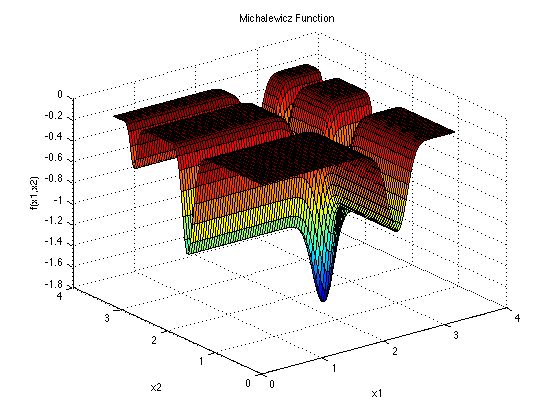
\includegraphics[width=0.7\linewidth]{img/python2} 

}

\caption{MICHALEWICZ FUNCTION}\label{fig:python2}
\end{figure}

\[
f(x)=-\sum_{i=1}^{d}sin(x_i)[sin(\frac{ix_i^2}{\pi})]^{2m}
\] Michalewicz function
有\(d!\)个局部极值,通常在\(x_i\in[0,\pi],i=1,\cdots,d\)内进行评价。

\begin{Shaded}
\begin{Highlighting}[]
\KeywordTok{class}\NormalTok{ mich(Problem):}
    \KeywordTok{def} \FunctionTok{__init__}\NormalTok{(}\VariableTok{self}\NormalTok{):}
        \BuiltInTok{super}\NormalTok{(mich, }\VariableTok{self}\NormalTok{).}\FunctionTok{__init__}\NormalTok{(nvars}\OperatorTok{=}\DecValTok{2}\NormalTok{, nobjs}\OperatorTok{=}\DecValTok{1}\NormalTok{)}
        \VariableTok{self}\NormalTok{.types[:] }\OperatorTok{=}\NormalTok{ [Real(}\OperatorTok{-}\DecValTok{6}\NormalTok{, }\OperatorTok{-}\DecValTok{1}\NormalTok{), Real(}\DecValTok{0}\NormalTok{, }\DecValTok{2}\NormalTok{)]}

    \KeywordTok{def}\NormalTok{ evaluate(}\VariableTok{self}\NormalTok{, solution):}
        \BuiltInTok{vars} \OperatorTok{=}\NormalTok{ solution.variables[:]}
\NormalTok{        x1 }\OperatorTok{=} \BuiltInTok{vars}\NormalTok{[}\DecValTok{0}\NormalTok{]}
\NormalTok{        x2 }\OperatorTok{=} \BuiltInTok{vars}\NormalTok{[}\DecValTok{1}\NormalTok{]}
\NormalTok{        y1 }\OperatorTok{=} \OperatorTok{-}\NormalTok{sin(x1) }\OperatorTok{*}\NormalTok{ ((sin((x1 }\OperatorTok{**} \DecValTok{2}\NormalTok{) }\OperatorTok{/}\NormalTok{ pi)) }\OperatorTok{**} \DecValTok{20}\NormalTok{)}
\NormalTok{        y2 }\OperatorTok{=} \OperatorTok{-}\NormalTok{sin(x2) }\OperatorTok{*}\NormalTok{ ((sin((}\DecValTok{2} \OperatorTok{*}\NormalTok{ x2 }\OperatorTok{**} \DecValTok{2}\NormalTok{) }\OperatorTok{/}\NormalTok{ pi)) }\OperatorTok{**} \DecValTok{20}\NormalTok{)}
\NormalTok{        solution.objectives[:] }\OperatorTok{=}\NormalTok{ [y1 }\OperatorTok{+}\NormalTok{ y2]}
\end{Highlighting}
\end{Shaded}

第三个问题是ACKLEY函数(ACKLEY FUNCTION)。

\begin{figure}

{\centering 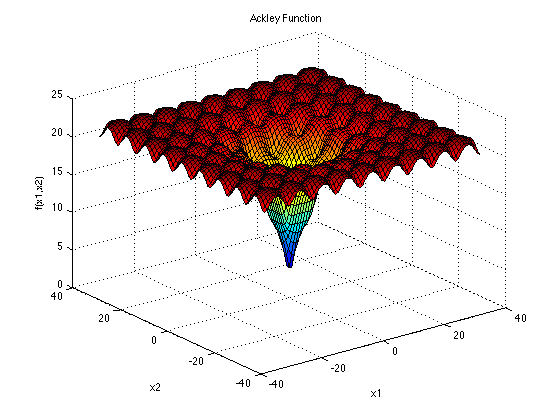
\includegraphics[width=0.7\linewidth]{img/python3} 

}

\caption{ACKLEY FUNCTION}\label{fig:python3}
\end{figure}

\[
f(x) = -aexp(-b\sqrt{\frac{1}{d}\sum_{i=1}^dx_i^2}-exp(\frac{1}{d}\sum_{i=1}^{d}cos(cx_i))+a+exp(1)
\] 推荐的测试参数为\(a=20,b=0.2,c=2\pi\),
\(x_i\in[-32.768,32.768],i=1,\cdots,d\)。
全局最小值为\(f(x^*)=0,\quad at\quad x^* = (0,\cdots,0)\)

\begin{Shaded}
\begin{Highlighting}[]
\KeywordTok{class}\NormalTok{ Ackley(Problem):}
    \KeywordTok{def} \FunctionTok{__init__}\NormalTok{(}\VariableTok{self}\NormalTok{):}
        \BuiltInTok{super}\NormalTok{(Ackley, }\VariableTok{self}\NormalTok{).}\FunctionTok{__init__}\NormalTok{(nvars}\OperatorTok{=}\DecValTok{2}\NormalTok{, nobjs}\OperatorTok{=}\DecValTok{1}\NormalTok{)}
        \VariableTok{self}\NormalTok{.types[:] }\OperatorTok{=}\NormalTok{ [Real(}\OperatorTok{-}\DecValTok{15}\NormalTok{, }\DecValTok{30}\NormalTok{), Real(}\OperatorTok{-}\DecValTok{15}\NormalTok{, }\DecValTok{20}\NormalTok{)]}

    \KeywordTok{def}\NormalTok{ evaluate(}\VariableTok{self}\NormalTok{, solution):}
        \BuiltInTok{vars} \OperatorTok{=}\NormalTok{ solution.variables[:]}
\NormalTok{        n }\OperatorTok{=} \DecValTok{2}
\NormalTok{        a }\OperatorTok{=} \DecValTok{20}
\NormalTok{        b }\OperatorTok{=} \FloatTok{0.2}
\NormalTok{        c }\OperatorTok{=} \DecValTok{2} \OperatorTok{*}\NormalTok{ pi}
\NormalTok{        s1 }\OperatorTok{=} \DecValTok{0}
\NormalTok{        s2 }\OperatorTok{=} \DecValTok{0}
        \ControlFlowTok{for}\NormalTok{ i }\KeywordTok{in} \BuiltInTok{range}\NormalTok{(n):}
\NormalTok{            s1 }\OperatorTok{=}\NormalTok{ s1 }\OperatorTok{+} \BuiltInTok{vars}\NormalTok{[i] }\OperatorTok{**} \DecValTok{2}
\NormalTok{            s2 }\OperatorTok{=}\NormalTok{ s2 }\OperatorTok{+}\NormalTok{ cos(c }\OperatorTok{*} \BuiltInTok{vars}\NormalTok{[i])}
\NormalTok{        y }\OperatorTok{=} \OperatorTok{-}\NormalTok{a }\OperatorTok{*}\NormalTok{ exp(}\OperatorTok{-}\NormalTok{b }\OperatorTok{*}\NormalTok{ sqrt(}\DecValTok{1} \OperatorTok{/}\NormalTok{ n }\OperatorTok{*}\NormalTok{ s1)) }\OperatorTok{-}\NormalTok{ exp(}\DecValTok{1} \OperatorTok{/}\NormalTok{ n }\OperatorTok{*}\NormalTok{ s2) }\OperatorTok{+}\NormalTok{ a }\OperatorTok{+}\NormalTok{ exp(}\DecValTok{1}\NormalTok{)}
\NormalTok{        solution.objectives[:] }\OperatorTok{=}\NormalTok{ [y]}
        
\end{Highlighting}
\end{Shaded}

然后我们将每个问题构成一个单独的实例。

\begin{Shaded}
\begin{Highlighting}[]
\NormalTok{problem }\OperatorTok{=}\NormalTok{ gold()}
\NormalTok{problem2 }\OperatorTok{=}\NormalTok{ mich()}
\NormalTok{problem3 }\OperatorTok{=}\NormalTok{ Ackley()}
\end{Highlighting}
\end{Shaded}

接下来,我们创建BAS算法的实例。BAS算法中需要修改一些参数来获得更好的结果。例如第一个BAS实例中step=1,c=5。完成初始化后,我们可以针对不同的问题迭代不同的次数,例如第三个BAS实例中,算法迭代了300次。最后通过print函数读取最优解。可以直接输出solution这个类,他的输出顺序是:

\textbf{Solution{[}solution.variables\textbar{}solution.objectives\textbar{}solution.constraints{]}}

\begin{Shaded}
\begin{Highlighting}[]
\NormalTok{algorithm }\OperatorTok{=}\NormalTok{ BAS(problem, step}\OperatorTok{=}\DecValTok{1}\NormalTok{, c}\OperatorTok{=}\DecValTok{5}\NormalTok{)}
\NormalTok{algorithm.run(}\DecValTok{100}\NormalTok{)}
\BuiltInTok{print}\NormalTok{(algorithm.best)}
\end{Highlighting}
\end{Shaded}

结果显示为:

\begin{verbatim}
Solution[-0.0024583254426162517,-1.002363921850713|3.0026888420039026|0]
\end{verbatim}

当然也可以直接输出目标函数,例如算法实例2。

\begin{Shaded}
\begin{Highlighting}[]
\NormalTok{algorithm2 }\OperatorTok{=}\NormalTok{ BAS(problem2, step}\OperatorTok{=}\DecValTok{5}\NormalTok{)}
\NormalTok{algorithm2.run(}\DecValTok{1000}\NormalTok{)}
\BuiltInTok{print}\NormalTok{(algorithm2.best.objectives)}
\end{Highlighting}
\end{Shaded}

结果显示为:

\begin{verbatim}
[-1.6524859808670134]
\end{verbatim}

或者也可以通过格式化的方法获得更好的输出效果

\begin{Shaded}
\begin{Highlighting}[]
\NormalTok{algorithm3 }\OperatorTok{=}\NormalTok{ BAS(problem3, step}\OperatorTok{=}\DecValTok{30}\NormalTok{, c}\OperatorTok{=}\FloatTok{0.1}\NormalTok{)}
\NormalTok{algorithm3.run(}\DecValTok{300}\NormalTok{)}
\BuiltInTok{print}\NormalTok{(}\StringTok{'Variables = }\SpecialCharTok{\{\}}\CharTok{\textbackslash{}n}\StringTok{Objective = }\SpecialCharTok{\{\}}\StringTok{'}\NormalTok{.}\BuiltInTok{format}\NormalTok{(algorithm3.best.variables,algorithm3.best.objectives))}
\end{Highlighting}
\end{Shaded}

结果显示为:

\begin{verbatim}
Variables = [1.52121543e-06 2.42423873e-06]
Objective = [8.095169530708546e-06]
\end{verbatim}

\chapter{Matlab用户}\label{matlabr}

之前一直有同学在群里面反映,有没有matlab用户可以使用rBAS的方法。尽管我曾经也是matlab的忠实用户,但现在能力退化严重,实在是写不动代码。加之,我认为学习R的成本很低,而且更加便捷。因此,也就熄了再去做一个matlab
toolbox的心思。

不过,我还是决定尝试下是否存在两者的接口,可以完成参数的传递,让使用matlab的同学也可以使用rBAS。于是有了下面几点思路。

\begin{itemize}
\tightlist
\item
  使用matlab,通过R(D)COM服务器来与R通讯,其配置对于R用户而言尚且显得麻烦,何况matlab用户。不过在看mathwork的网站时,倒是得知他们把R
  interface作为了未来的开发计划之一。所以,日后可以采用在matlab中调用R的形式。目前尚无此功能。
\item
  使用R中的R.matlab包,来与matlab通讯。这个办法咋一看很简单,尝试也成功了。最大的问题是\textbf{慢},其次看源码应该是要配置\textbf{Java}(我电脑上原本有,执行无碍,但没有删除Java后尝试)。这种慢,可以称为很慢,后面我们能见识到。
\item
  使用\textbf{第三方语言},如C/C++。别害怕,因为matlab提供了很强大的工具,即\texttt{Matlab\ Coder}来把你的matlab代码转为C或者C++。
\end{itemize}

下面我们讲第二点和第三点是如何操作的。

\section{使用R.matlab包}\label{r.matlab}

这一节更类似于娱乐和探索。因为该方法用于优化求解的速度,真的让人难以接受(也有可能是我没有找对方法)。如果无意于此,可以跳过。

首先,可以按照下面的代码从CRAN安装该包。

\begin{Shaded}
\begin{Highlighting}[]
\KeywordTok{install.packages}\NormalTok{(}\StringTok{'R.matlab'}\NormalTok{)}
\end{Highlighting}
\end{Shaded}

当然,也可以利用\texttt{devtools}从github上按照该包。

\begin{Shaded}
\begin{Highlighting}[]
\NormalTok{devtools}\OperatorTok{::}\KeywordTok{install_github}\NormalTok{(}\StringTok{'HenrikBengtsson/R.matlab'}\NormalTok{)}
\end{Highlighting}
\end{Shaded}

接下来,按照\href{https://cran.r-project.org/web/packages/R.matlab/R.matlab.pdf}{包的文档}进行操作。

首先,加载包。

\begin{Shaded}
\begin{Highlighting}[]
\KeywordTok{library}\NormalTok{(}\StringTok{'R.matlab'}\NormalTok{)}
\end{Highlighting}
\end{Shaded}

在R中打开\texttt{matlab\ server}。

\begin{Shaded}
\begin{Highlighting}[]
\NormalTok{Matlab}\OperatorTok{$}\KeywordTok{startServer}\NormalTok{()}
\end{Highlighting}
\end{Shaded}

效果就是可以看到matlab窗口以最小化的形式出现,不过里面没有视图,大家可以不必理会。后续操作均在R中完成。

其次创建matlab对象,用于与Matlab通讯。

\begin{Shaded}
\begin{Highlighting}[]
\NormalTok{matlab <-}\StringTok{ }\KeywordTok{Matlab}\NormalTok{()}
\end{Highlighting}
\end{Shaded}

然后,把要优化的函数(\textbf{使用matlab定义}),写入R。

\begin{Shaded}
\begin{Highlighting}[]
\KeywordTok{setFunction}\NormalTok{(matlab, }\StringTok{" \textbackslash{}}
\StringTok{  function z=test(x) \textbackslash{}}
\StringTok{            %test function \textbackslash{}}
\StringTok{            z = 100 *(x(2) - x(1).^2).^2+(x(1)-1).^2;\textbackslash{}}
\StringTok{            "}\NormalTok{)}
\end{Highlighting}
\end{Shaded}

这段代码,在matlab的本地服务器创建了一个M函数,如下所示。注意用\texttt{\textbackslash{}}号的使用。

\begin{Shaded}
\begin{Highlighting}[]
\NormalTok{function z =test(x,y)}
  \CommentTok{%test function}
\NormalTok{  z=}\FloatTok{100}\NormalTok{*(y-x.^}\FloatTok{2}\NormalTok{).^}\FloatTok{2}\NormalTok{+(x-}\FloatTok{1}\NormalTok{).^}\FloatTok{2}\NormalTok{;}
\end{Highlighting}
\end{Shaded}

接下来我们创建目标函数。

\begin{Shaded}
\begin{Highlighting}[]
\NormalTok{func_MR <-}\StringTok{ }\ControlFlowTok{function}\NormalTok{(x)\{}
  \KeywordTok{setVariable}\NormalTok{(matlab,}\DataTypeTok{x =}\NormalTok{ x) }\CommentTok{# 把R里面的x,赋值到matlab里面的x变量}
  \KeywordTok{evaluate}\NormalTok{(matlab,}\StringTok{'z = test(x)'}\NormalTok{) }\CommentTok{# 在matlab里面执行 z = test(x) 命令}
\NormalTok{  res <-}\StringTok{ }\KeywordTok{getVariable}\NormalTok{(matlab,}\KeywordTok{c}\NormalTok{(}\StringTok{'z'}\NormalTok{)) }\CommentTok{# 从matlab里面读取 z 变量}
  \KeywordTok{return}\NormalTok{(res}\OperatorTok{$}\NormalTok{z) }\CommentTok{#返回z值}
\NormalTok{\}}
\end{Highlighting}
\end{Shaded}

这段代码块思路是,既然利用的是rBAS包,那么每次更新,都利用上一回合R计算的值,传递到matlab里面。然后,在matlab里面执行用户定义的函数。最后再用R把matlab里面算出来的变量值读取出来。

这就是我们新的优化函数,虽然绕一点,但是是容易想到和理解的办法。接下来就是使用rBAS包来优化这个目标函数了。

\begin{Shaded}
\begin{Highlighting}[]
\KeywordTok{system.time}\NormalTok{(\{}
\NormalTok{  fit<-}
\StringTok{    }\KeywordTok{BSOoptim}\NormalTok{(}\DataTypeTok{fn =}\NormalTok{ func_MR,}
             \DataTypeTok{init =} \OtherTok{NULL}\NormalTok{,}
             \DataTypeTok{s =} \DecValTok{2}\NormalTok{,}
             \DataTypeTok{lower =} \KeywordTok{c}\NormalTok{(}\OperatorTok{-}\DecValTok{50}\NormalTok{,}\OperatorTok{-}\DecValTok{50}\NormalTok{),}
             \DataTypeTok{upper =} \KeywordTok{c}\NormalTok{(}\DecValTok{50}\NormalTok{,}\DecValTok{50}\NormalTok{),}
             \DataTypeTok{n =} \DecValTok{1}\NormalTok{,}
             \DataTypeTok{w =} \KeywordTok{c}\NormalTok{(}\FloatTok{0.9}\NormalTok{,}\FloatTok{0.4}\NormalTok{),}
             \DataTypeTok{w_vs =} \FloatTok{0.4}\NormalTok{, }
             \DataTypeTok{step =} \DecValTok{10}\NormalTok{,}
             \DataTypeTok{step_w =} \KeywordTok{c}\NormalTok{(}\FloatTok{0.9}\NormalTok{,}\FloatTok{0.4}\NormalTok{),}
             \DataTypeTok{c =} \DecValTok{8}\NormalTok{,}
             \DataTypeTok{v =} \KeywordTok{c}\NormalTok{(}\OperatorTok{-}\FloatTok{5.12}\NormalTok{,}\FloatTok{5.12}\NormalTok{),}
             \DataTypeTok{trace =}\NormalTok{ T,}\DataTypeTok{seed =} \DecValTok{1}\NormalTok{)}
\NormalTok{\}) }
\end{Highlighting}
\end{Shaded}

我们使用了一段\texttt{BSO}算法的优化代码,但是,粒子数目设置为2,回合数只设置为1。结果,这么简单的计算,要花费\textbf{13s}。两个软件来回通讯占用了大量的时间,我相信,应该不会有用户愿意等待这么长久的时间。这个完整的优化过程,之后会有纯R代码,求解过程不到0.1s的时间。

最后呢,需要使用下面的代码关闭matlab服务器。

\begin{Shaded}
\begin{Highlighting}[]
\KeywordTok{close}\NormalTok{(matlab)}
\end{Highlighting}
\end{Shaded}

R代码使用\texttt{BSO}解这个优化问题是这样的效果。

\begin{Shaded}
\begin{Highlighting}[]
\KeywordTok{library}\NormalTok{(rBAS)}

\NormalTok{test <-}\StringTok{ }\ControlFlowTok{function}\NormalTok{(x)\{}
\NormalTok{  z <-}\StringTok{ }\DecValTok{100}\OperatorTok{*}\NormalTok{(x[}\DecValTok{2}\NormalTok{]}\OperatorTok{-}\NormalTok{x[}\DecValTok{1}\NormalTok{]}\OperatorTok{^}\DecValTok{2}\NormalTok{)}\OperatorTok{^}\DecValTok{2} \OperatorTok{+}\StringTok{ }\NormalTok{(x[}\DecValTok{1}\NormalTok{] }\OperatorTok{-}\StringTok{ }\DecValTok{1}\NormalTok{)}\OperatorTok{^}\DecValTok{2}
\NormalTok{\}}

\KeywordTok{system.time}\NormalTok{(\{}
\NormalTok{  fit<-}
\StringTok{    }\KeywordTok{BSOoptim}\NormalTok{(}\DataTypeTok{fn =}\NormalTok{ test,}
             \DataTypeTok{init =} \OtherTok{NULL}\NormalTok{,}
             \DataTypeTok{lower =} \KeywordTok{c}\NormalTok{(}\OperatorTok{-}\DecValTok{50}\NormalTok{,}\OperatorTok{-}\DecValTok{50}\NormalTok{),}
             \DataTypeTok{upper =} \KeywordTok{c}\NormalTok{(}\DecValTok{50}\NormalTok{,}\DecValTok{50}\NormalTok{),}
             \DataTypeTok{n =} \DecValTok{300}\NormalTok{,}
             \DataTypeTok{w =} \KeywordTok{c}\NormalTok{(}\FloatTok{0.9}\NormalTok{,}\FloatTok{0.4}\NormalTok{),}
             \DataTypeTok{w_vs =} \FloatTok{0.4}\NormalTok{, }
             \DataTypeTok{step =} \DecValTok{10}\NormalTok{,}
             \DataTypeTok{step_w =} \KeywordTok{c}\NormalTok{(}\FloatTok{0.9}\NormalTok{,}\FloatTok{0.4}\NormalTok{),}
             \DataTypeTok{c =} \DecValTok{8}\NormalTok{,}
             \DataTypeTok{v =} \KeywordTok{c}\NormalTok{(}\OperatorTok{-}\FloatTok{5.12}\NormalTok{,}\FloatTok{5.12}\NormalTok{),}
             \DataTypeTok{trace =}\NormalTok{ F,}\DataTypeTok{seed =} \DecValTok{1}\NormalTok{)}
\NormalTok{\})}
\end{Highlighting}
\end{Shaded}

\begin{verbatim}
##    user  system elapsed 
##    0.12    0.00    0.12
\end{verbatim}

\begin{Shaded}
\begin{Highlighting}[]
\NormalTok{fit}\OperatorTok{$}\NormalTok{par}
\end{Highlighting}
\end{Shaded}

\begin{verbatim}
## [1] 1 1
\end{verbatim}

\begin{Shaded}
\begin{Highlighting}[]
\NormalTok{fit}\OperatorTok{$}\NormalTok{value}
\end{Highlighting}
\end{Shaded}

\begin{verbatim}
## [1] 0
\end{verbatim}

时间短,而且能求出理论的最小值。这也反映了第二个方法过于低效的问题,我们看看借助第三方语言能否行得通。

\section{中转站:C/C++}\label{cc}

matlab的\texttt{matlab\ Coder}可以让用户把自己的代码变成C或者C++,前提是,需要有编译器。不过,如果你使用过R,那么一般都会安装\href{https://cran.r-project.org/bin/windows/Rtools/}{Rtools},这就意味着你安装了MinGw。下面的过程需要用到Rtools,还请大家自行下载安装。

打开matlab,输入下面的指令:

\begin{Shaded}
\begin{Highlighting}[]
\NormalTok{mex -steup}
\end{Highlighting}
\end{Shaded}

如果电脑中只安装过Rtools,而没有VS之类的编译器,一般会显示图\ref{fig:mex}的界面。

\begin{figure}

{\centering 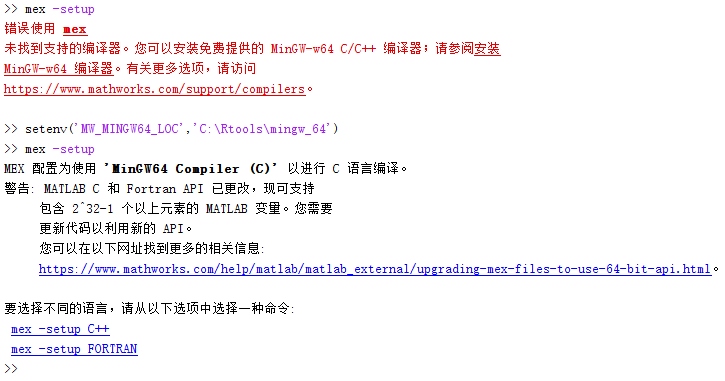
\includegraphics[width=0.95\linewidth]{img/mex} 

}

\caption{mex -setup}\label{fig:mex}
\end{figure}

第一句报错,是因为我并没有把Rtools中的mingw\_64文件夹加入环境变量。因此,在执行第二句之后,再执行\texttt{mex\ -setup}就不会报错。

好了,加入你成功了,那么抛开前面所有的知识不看。现在说Coder工具箱。

假设你的路径下有2个M文件,一个是我们之前所说的测试函数\texttt{test.m},还有一个是我们所说的,用来测试\texttt{test}函数的文件\texttt{test\_main.m}文件。它们的代码如下。

\begin{Shaded}
\begin{Highlighting}[]
\CommentTok

\NormalTok{function z = test(x)}
\NormalTok{z = }\FloatTok{100}\NormalTok{ *(x(}\FloatTok{2}\NormalTok{) - x(}\FloatTok{1}\NormalTok{).^}\FloatTok{2}\NormalTok{).^}\FloatTok{2}\NormalTok{+(x(}\FloatTok{1}\NormalTok{)-}\FloatTok{1}\NormalTok{).^}\FloatTok{2}\NormalTok{;}
\end{Highlighting}
\end{Shaded}

\begin{Shaded}
\begin{Highlighting}[]
\CommentTok

\NormalTok{z = test([}\FloatTok{1} \FloatTok{1}\NormalTok{]);}
\end{Highlighting}
\end{Shaded}

接下来我们点击Matlab菜单栏上的APP,在里面找到Matlab
Coder工具箱打开,如图\ref{fig:coder1}。

\begin{figure}

{\centering 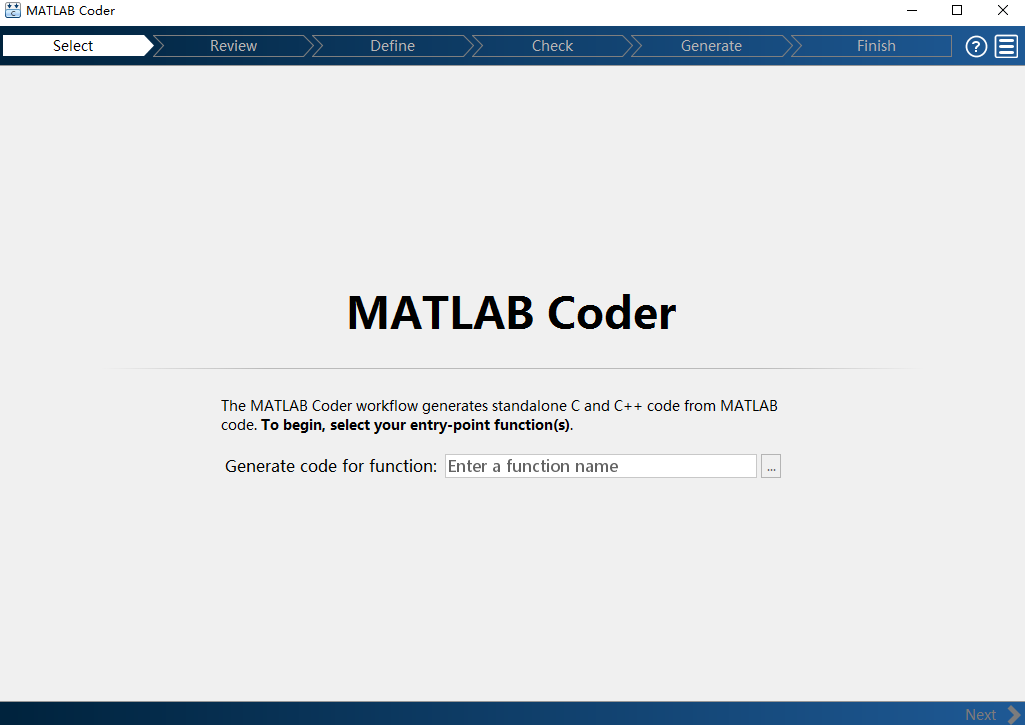
\includegraphics[width=0.95\linewidth]{img/coder1} 

}

\caption{Matlab Coder}\label{fig:coder1}
\end{figure}

点击Enter a function name右边的
\(\cdots\)符号,然后选中\texttt{test.m}文件,可以看到图\ref{fig:coder2}的效果。

\begin{figure}

{\centering 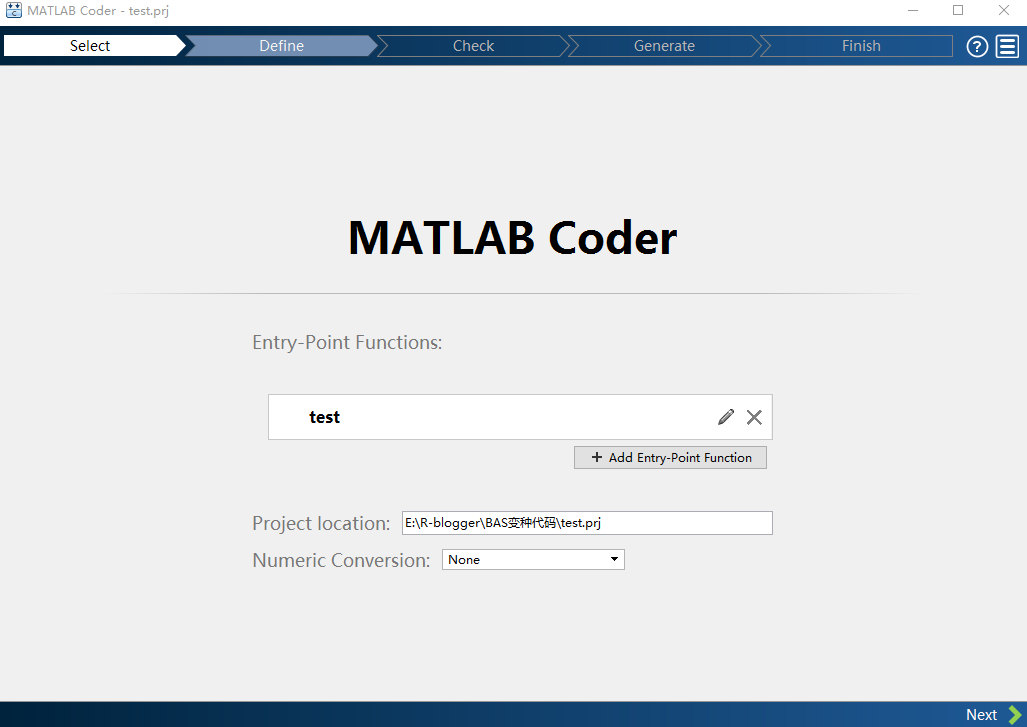
\includegraphics[width=0.95\linewidth]{img/coder2} 

}

\caption{Matlab Coder}\label{fig:coder2}
\end{figure}

点击右下角\texttt{Next}按钮,可以看到如图\ref{fig:coder3}的界面。

\begin{figure}

{\centering 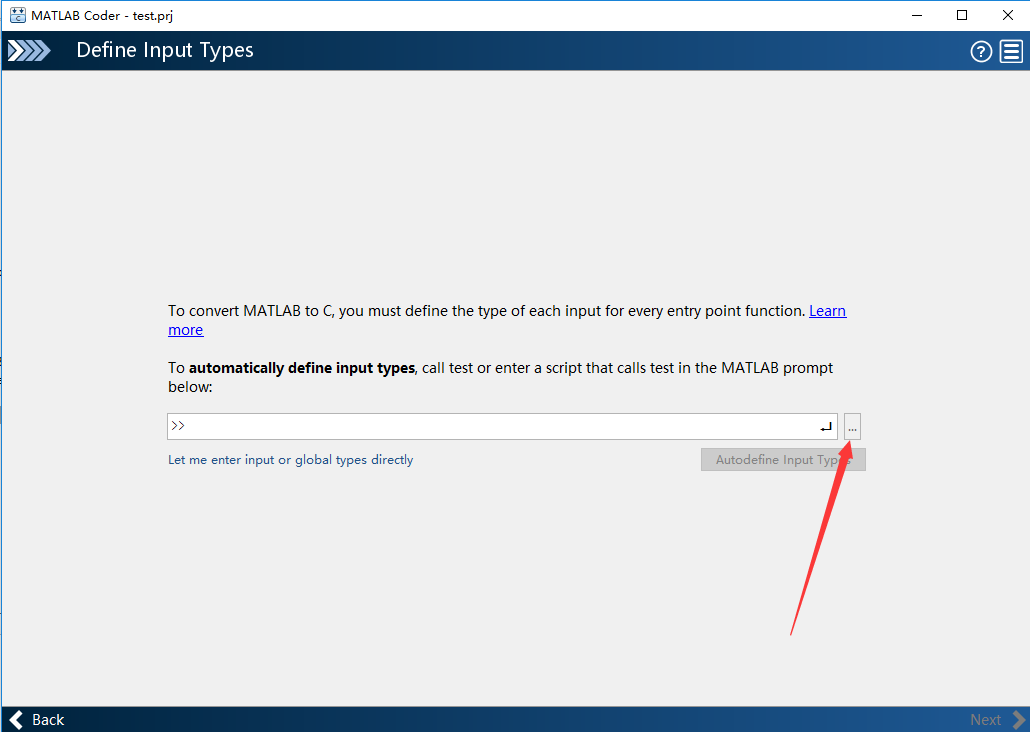
\includegraphics[width=0.95\linewidth]{img/coder3} 

}

\caption{Matlab Coder}\label{fig:coder3}
\end{figure}

点击图\ref{fig:coder3}红色箭头所指处,并选中\texttt{test\_main.m}文件,点击\texttt{Autodefine\ Input\ types},可以看到如图\ref{fig:coder4}的界面,接下来就是一路的\texttt{Next}。

\begin{figure}

{\centering 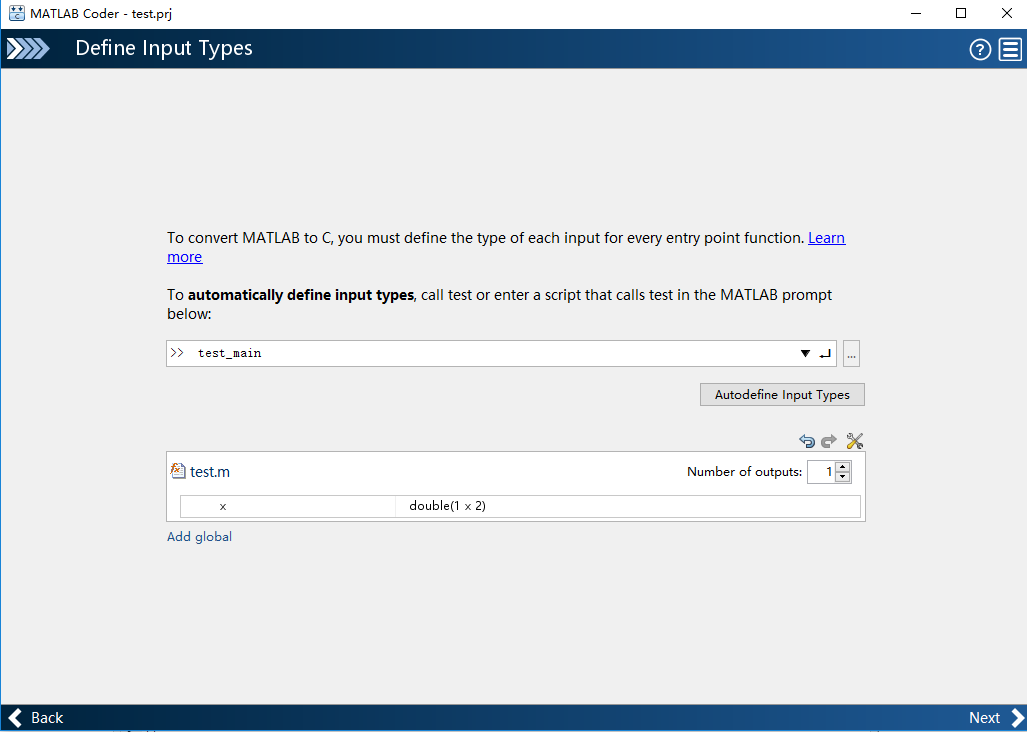
\includegraphics[width=0.95\linewidth]{img/coder4} 

}

\caption{Matlab Coder}\label{fig:coder4}
\end{figure}

\begin{figure}

{\centering 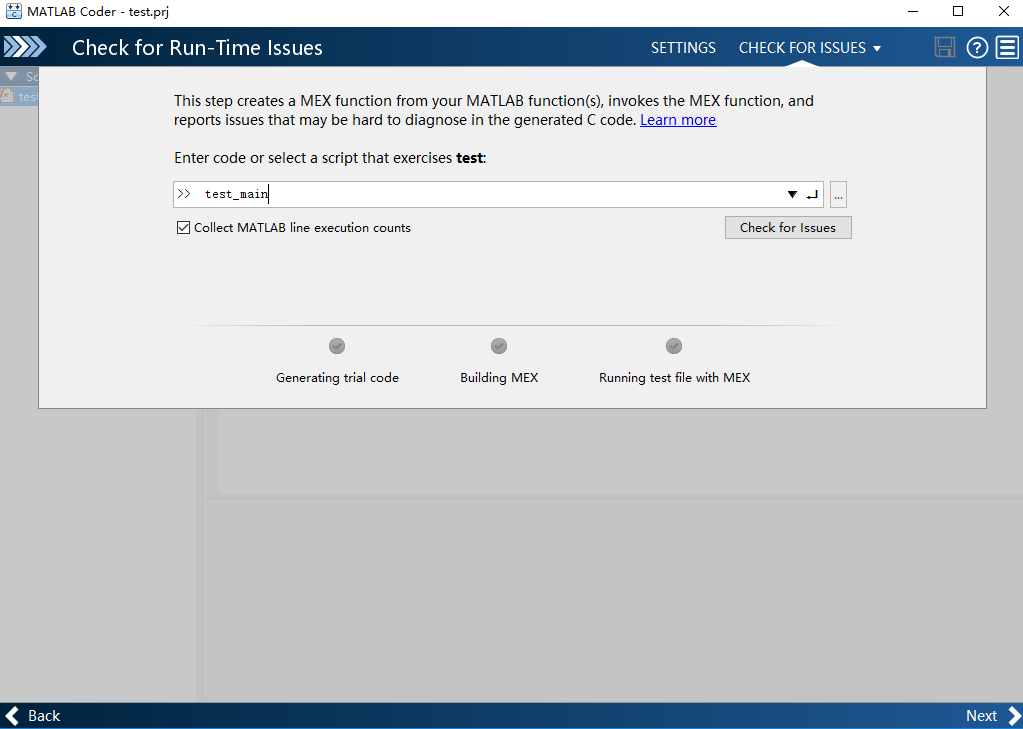
\includegraphics[width=0.95\linewidth]{img/coder5} 

}

\caption{Matlab Coder}\label{fig:coder5}
\end{figure}

直到图\ref{fig:coder6},点击\texttt{Generate}按钮,生成C代码。

\begin{figure}

{\centering 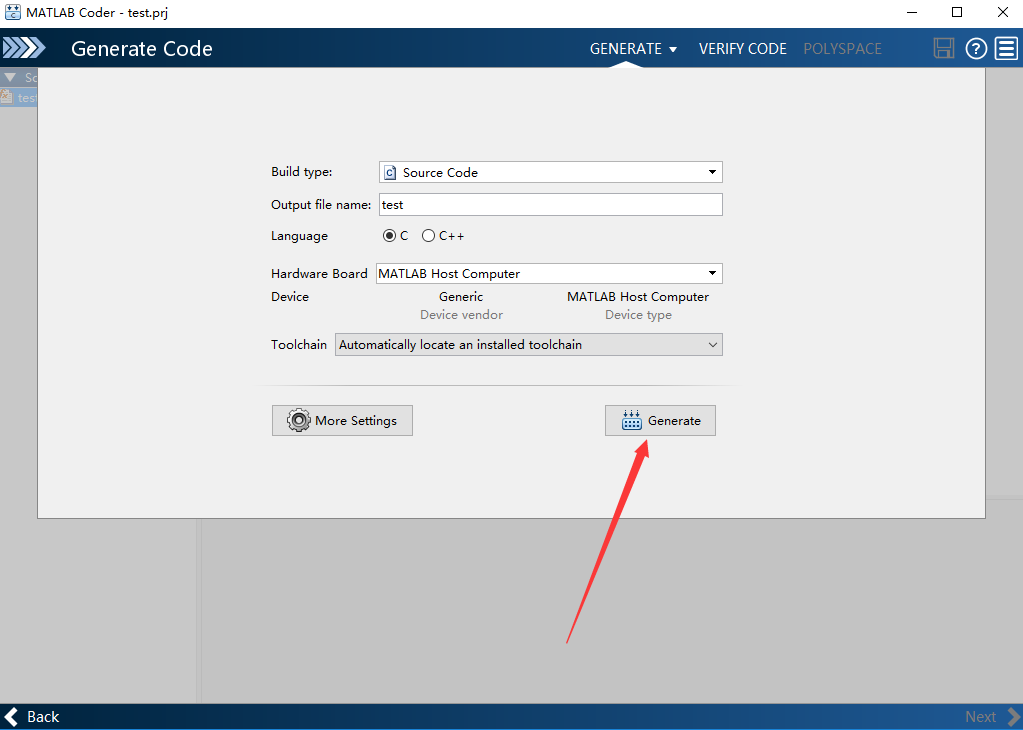
\includegraphics[width=0.95\linewidth]{img/coder6} 

}

\caption{Matlab Coder}\label{fig:coder6}
\end{figure}

而后工具箱会给出\texttt{test.c}代码的预览,如图\ref{fig:coder7}。

\begin{figure}

{\centering 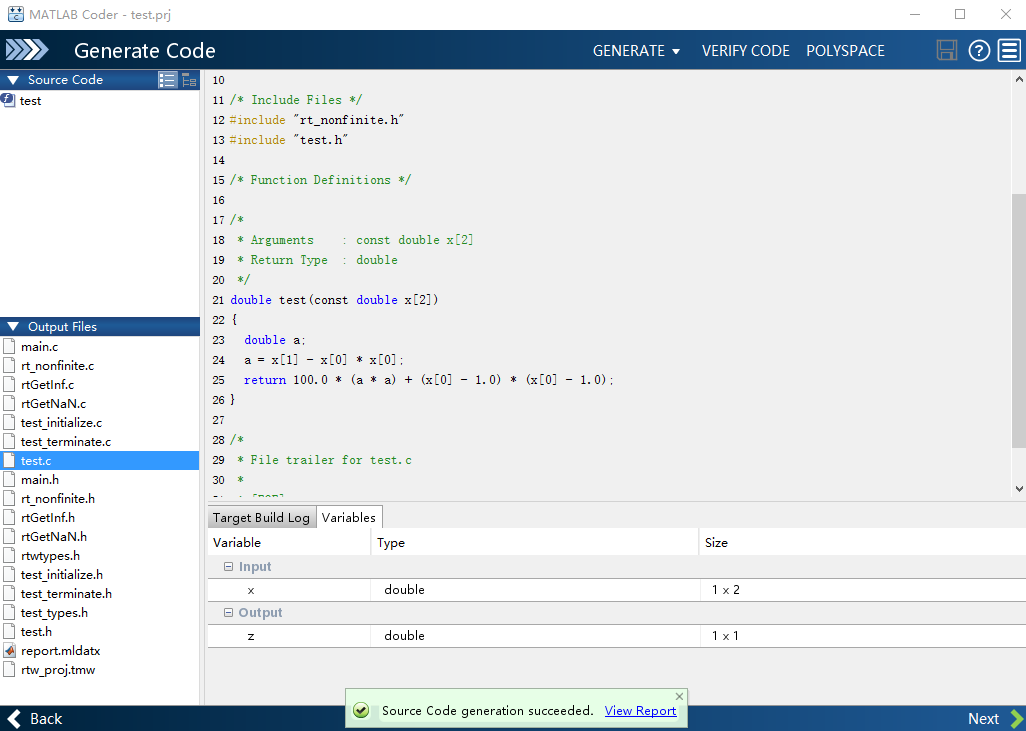
\includegraphics[width=0.95\linewidth]{img/coder7} 

}

\caption{Matlab Coder}\label{fig:coder7}
\end{figure}

我相信,大家还是能看懂这段代码。对于简单的优化问题,我们照猫画虎,就可以写出对应的C或者C++的代码。如果不想写,还可以按照上述的方法生成。

那现在问题来了,如果我们有了C代码,如何在R语言中用了。

由于matlab生成的代码很多库都是matlab依赖的(我这么认为,不一定正确),所以我们需要简单地调整一下,把代码变得简洁。

原始的代码是这样的。

\begin{Shaded}
\begin{Highlighting}[]
\CommentTok{/* Include Files */}
\PreprocessorTok{#include }\ImportTok{"rt_nonfinite.h"}
\PreprocessorTok{#include }\ImportTok{"test.h"}

\CommentTok{/* Function Definitions */}

\CommentTok{/*}
\CommentTok{ * Arguments    : const double x[2]}
\CommentTok{ * Return Type  : double}
\CommentTok{ */}
\DataTypeTok{double}\NormalTok{ test(}\DataTypeTok{const} \DataTypeTok{double}\NormalTok{ x[}\DecValTok{2}\NormalTok{])}
\NormalTok{\{}
  \DataTypeTok{double}\NormalTok{ a;}
\NormalTok{  a = x[}\DecValTok{1}\NormalTok{] - x[}\DecValTok{0}\NormalTok{] * x[}\DecValTok{0}\NormalTok{];}
  \ControlFlowTok{return} \FloatTok{100.0}\NormalTok{ * (a * a) + (x[}\DecValTok{0}\NormalTok{] - }\FloatTok{1.0}\NormalTok{) * (x[}\DecValTok{0}\NormalTok{] - }\FloatTok{1.0}\NormalTok{);}
\NormalTok{\}}

\CommentTok{/*}
\CommentTok{ * File trailer for test.c}
\CommentTok{ *}
\CommentTok{ * [EOF]}
\CommentTok{ */}
\end{Highlighting}
\end{Shaded}

我们进行\textbf{微调}(大家肯定是能理解并模仿的),变成R可以正确编译的。注意,由于Rcpp能让R和C++无缝贴合的强大功能,我把代码调整为了C++。后面的\texttt{Michalewicz\ function},\texttt{Pressure\ Vessel\ function}均是用C++所写。

\begin{verbatim}
#include <Rcpp.h>
using namespace Rcpp;
// [[Rcpp::export]]
double test(NumericVector x) {
  double a;
  a = x[1] - x[0] * x[0];
  return 100.0 * (a*a) + (x[0] - 1.0) * (x[0] - 1.0);
}
\end{verbatim}

把这段代码保存成\texttt{Rcpptest.cpp}文件,然后在R里面执行代码:

\begin{Shaded}
\begin{Highlighting}[]
\KeywordTok{library}\NormalTok{(Rcpp) }\CommentTok{#加载Rcpp包}
\KeywordTok{sourceCpp}\NormalTok{(}\StringTok{'你的Rcpptest.cpp文件路径'}\NormalTok{) }\CommentTok{#编译之前保存的cpp文件}
\end{Highlighting}
\end{Shaded}

\begin{Shaded}
\begin{Highlighting}[]
\CommentTok{#执行BSO优化算法函数}
\KeywordTok{system.time}\NormalTok{(\{}
\NormalTok{  fit<-}\KeywordTok{BSOoptim}\NormalTok{(}\DataTypeTok{fn =}\NormalTok{ test, }\CommentTok{#调用了编译的C++中的test函数}
                \DataTypeTok{init =} \OtherTok{NULL}\NormalTok{,}
                \DataTypeTok{lower =} \KeywordTok{c}\NormalTok{(}\OperatorTok{-}\DecValTok{50}\NormalTok{,}\OperatorTok{-}\DecValTok{50}\NormalTok{),}
                \DataTypeTok{upper =} \KeywordTok{c}\NormalTok{(}\DecValTok{50}\NormalTok{,}\DecValTok{50}\NormalTok{),}
                \DataTypeTok{n =} \DecValTok{300}\NormalTok{,}
                \DataTypeTok{w =} \KeywordTok{c}\NormalTok{(}\FloatTok{0.9}\NormalTok{,}\FloatTok{0.4}\NormalTok{),}
                \DataTypeTok{w_vs =} \FloatTok{0.4}\NormalTok{, }
                \DataTypeTok{step =} \DecValTok{10}\NormalTok{,}
                \DataTypeTok{step_w =} \KeywordTok{c}\NormalTok{(}\FloatTok{0.9}\NormalTok{,}\FloatTok{0.4}\NormalTok{),}
                \DataTypeTok{c =} \DecValTok{8}\NormalTok{,}
                \DataTypeTok{v =} \KeywordTok{c}\NormalTok{(}\OperatorTok{-}\FloatTok{5.12}\NormalTok{,}\FloatTok{5.12}\NormalTok{),}
                \DataTypeTok{trace =}\NormalTok{ F,}\DataTypeTok{seed =} \DecValTok{1}\NormalTok{)}
\NormalTok{\})}
\end{Highlighting}
\end{Shaded}

\begin{verbatim}
##    user  system elapsed 
##    0.13    0.00    0.13
\end{verbatim}

\begin{Shaded}
\begin{Highlighting}[]
\CommentTok{#查看优化参数}
\NormalTok{fit}\OperatorTok{$}\NormalTok{par}
\end{Highlighting}
\end{Shaded}

\begin{verbatim}
## [1] 1 1
\end{verbatim}

\begin{Shaded}
\begin{Highlighting}[]
\CommentTok{#查看优化结果}
\NormalTok{fit}\OperatorTok{$}\NormalTok{value}
\end{Highlighting}
\end{Shaded}

\begin{verbatim}
## [1] 0
\end{verbatim}

执行速度很快,大家可能会有疑问,为啥看起来比纯R代码执行的时间还要长一点。这是因为你多次执行,耗时和电脑所处的状态有关系,这点误差是正常的。但是,如果是计算量较大的代码,利\textbf{用Rcpp会比R要节省大量的时间}。

接下来我们看看另外两个例子,也就是\texttt{Michalewicz\ function}和\texttt{Pressure\ Vessel\ function}函数的优化问题。

\texttt{Michalewicz\ function}
也可以先用matlab生成C或者C++代码,然后稍作改编,保存为\texttt{Rcppmich.cpp}文件,代码如下:

\begin{verbatim}
#include <Rcpp.h>
using namespace Rcpp;

// [[Rcpp::export]]
double michcpp(NumericVector x) {
  double x0;
  double x1;
  x0 = -sin(x[0])*pow(sin((pow(x[0],2))/M_PI),20);
  x1 = -sin(x[1])*pow(sin((2*pow(x[1],2))/M_PI),20);
  return x0+x1;
}
\end{verbatim}

和matlab或者R代码比起来,也是十分易懂的。

\begin{Shaded}
\begin{Highlighting}[]
\KeywordTok{library}\NormalTok{(Rcpp) }\CommentTok{#加载Rcpp包}
\KeywordTok{sourceCpp}\NormalTok{(}\StringTok{'你的Rcppmich.cpp文件路径'}\NormalTok{) }\CommentTok{#编译之前保存的cpp文件}
\end{Highlighting}
\end{Shaded}

\begin{Shaded}
\begin{Highlighting}[]
\CommentTok{#执行BAS优化算法函数}
\KeywordTok{system.time}\NormalTok{(\{}
\NormalTok{  fit<-}\KeywordTok{BASoptim}\NormalTok{(}\DataTypeTok{fn =}\NormalTok{ michcpp, }\CommentTok{#利用了C++中的michcpp函数}
                \DataTypeTok{lower =} \KeywordTok{c}\NormalTok{(}\OperatorTok{-}\DecValTok{6}\NormalTok{,}\DecValTok{0}\NormalTok{), }\DataTypeTok{upper =} \KeywordTok{c}\NormalTok{(}\OperatorTok{-}\DecValTok{1}\NormalTok{,}\DecValTok{2}\NormalTok{),}
                \DataTypeTok{seed =} \DecValTok{1}\NormalTok{, }\DataTypeTok{n =} \DecValTok{100}\NormalTok{,}\DataTypeTok{trace =} \OtherTok{FALSE}\NormalTok{)}
\NormalTok{\})}
\end{Highlighting}
\end{Shaded}

\begin{verbatim}
##    user  system elapsed 
##       0       0       0
\end{verbatim}

\begin{Shaded}
\begin{Highlighting}[]
\CommentTok{#查看优化参数}
\NormalTok{fit}\OperatorTok{$}\NormalTok{par}
\end{Highlighting}
\end{Shaded}

\begin{verbatim}
## [1] -4.964687  1.575415
\end{verbatim}

\begin{Shaded}
\begin{Highlighting}[]
\CommentTok{#查看优化结果}
\NormalTok{fit}\OperatorTok{$}\NormalTok{value}
\end{Highlighting}
\end{Shaded}

\begin{verbatim}
## [1] -1.966817
\end{verbatim}

对于\texttt{Pressure\ Vessel\ function},保存为\texttt{RcppPV.cpp}文件,代码如下:

\begin{verbatim}
#include <Rcpp.h>
using namespace Rcpp;

// [[Rcpp::export]]
double PVobj(NumericVector x) {
  double x0 = floor(x[0])*0.0625;
  double x1 = floor(x[1])*0.0625;
  double x2 = x[2];
  double x3 = x[3];
  
  double result = 0.6224*x0*x2*x3 + 1.7781*x1*pow(x2,2) 
    +3.1611*pow(x0,2)*x3 + 19.84*pow(x0,2)*x2;
  return result;
}

// [[Rcpp::export]]
NumericVector PVcon(NumericVector x) {
  double x0 = floor(x[0])*0.0625;
  double x1 = floor(x[1])*0.0625;
  double x2 = x[2];
  double x3 = x[3];
  
  NumericVector constraint(3);
  constraint[0] = 0.0193*x2 - x0;
  constraint[1] = 0.00954*x2 - x1;
  constraint[2] = 750.0*1728.0 - 3.141593*pow(x2,2)*x3 
    - (4.0/3.0)*3.141593*pow(x2,3);
  return constraint;
}
\end{verbatim}

其中,\texttt{PVobj}是目标函数,\texttt{PVcon}是约束函数。

\begin{Shaded}
\begin{Highlighting}[]
\KeywordTok{library}\NormalTok{(Rcpp) }\CommentTok{#加载Rcpp包}
\KeywordTok{sourceCpp}\NormalTok{(}\StringTok{'你的RcppPV.cpp文件路径'}\NormalTok{) }\CommentTok{#编译之前保存的cpp文件}
\end{Highlighting}
\end{Shaded}

\begin{Shaded}
\begin{Highlighting}[]
\CommentTok{#执行BSO优化算法函数}
\KeywordTok{system.time}\NormalTok{(\{}
\NormalTok{  fit<-}\KeywordTok{BSOoptim}\NormalTok{(}\DataTypeTok{fn =}\NormalTok{ PVobj, }\CommentTok{#C++中的PVobj函数}
         \DataTypeTok{init =} \OtherTok{NULL}\NormalTok{,}
         \DataTypeTok{constr =}\NormalTok{ PVcon, }\CommentTok{#C++中的PVcon函数}
         \DataTypeTok{lower =} \KeywordTok{c}\NormalTok{( }\DecValTok{1}\NormalTok{, }\DecValTok{1}\NormalTok{, }\DecValTok{10}\NormalTok{, }\DecValTok{10}\NormalTok{),}
         \DataTypeTok{upper =} \KeywordTok{c}\NormalTok{(}\DecValTok{100}\NormalTok{, }\DecValTok{100}\NormalTok{, }\DecValTok{200}\NormalTok{, }\DecValTok{200}\NormalTok{),}
         \DataTypeTok{n =} \DecValTok{1000}\NormalTok{,}
         \DataTypeTok{w =} \KeywordTok{c}\NormalTok{(}\FloatTok{0.9}\NormalTok{,}\FloatTok{0.4}\NormalTok{),}
         \DataTypeTok{w_vs =} \FloatTok{0.9}\NormalTok{,}
         \DataTypeTok{step =} \DecValTok{100}\NormalTok{,}
         \DataTypeTok{step_w =} \KeywordTok{c}\NormalTok{(}\FloatTok{0.9}\NormalTok{,}\FloatTok{0.4}\NormalTok{),}
         \DataTypeTok{c =} \DecValTok{35}\NormalTok{,}
         \DataTypeTok{v =} \KeywordTok{c}\NormalTok{(}\OperatorTok{-}\FloatTok{5.12}\NormalTok{,}\FloatTok{5.12}\NormalTok{),}
         \DataTypeTok{trace =}\NormalTok{ F,}\DataTypeTok{seed =} \DecValTok{1}\NormalTok{,}
         \DataTypeTok{pen =} \FloatTok{1e6}\NormalTok{)}
\NormalTok{\})}
\end{Highlighting}
\end{Shaded}

\begin{verbatim}
##    user  system elapsed 
##    1.96    0.00    1.95
\end{verbatim}

\begin{Shaded}
\begin{Highlighting}[]
\CommentTok{#查看优化参数}
\NormalTok{fit}\OperatorTok{$}\NormalTok{par}
\end{Highlighting}
\end{Shaded}

\begin{verbatim}
## [1]  13.948846   7.541387  42.098446 176.636570
\end{verbatim}

\begin{Shaded}
\begin{Highlighting}[]
\CommentTok{#查看优化结果}
\NormalTok{fit}\OperatorTok{$}\NormalTok{value}
\end{Highlighting}
\end{Shaded}

\begin{verbatim}
## [1] 6059.131
\end{verbatim}

结果很好,耗时也可以接受。不过,在写\texttt{BSOoptim}函数的时候,我使用了2层的循环来嵌套,因此,\texttt{BSOoptim}函数比rBAS包中其他的函数要慢上一些。后续我打算使用Rcpp把\texttt{BSOoptim}重写一遍,这样对大型的优化问题耗时会更容易接受。

下面是\texttt{BSASoptim}对该问题的优化结果,同样也是采用C++编译的方式。

\begin{Shaded}
\begin{Highlighting}[]
\KeywordTok{system.time}\NormalTok{(\{}
\NormalTok{  result <-}\StringTok{ }\KeywordTok{BSASoptim}\NormalTok{(}\DataTypeTok{fn =}\NormalTok{ PVobj,}
                      \DataTypeTok{k =} \DecValTok{5}\NormalTok{,}
                      \DataTypeTok{lower =}\KeywordTok{c}\NormalTok{( }\DecValTok{1}\NormalTok{, }\DecValTok{1}\NormalTok{, }\DecValTok{10}\NormalTok{, }\DecValTok{10}\NormalTok{),}
                      \DataTypeTok{upper =} \KeywordTok{c}\NormalTok{(}\DecValTok{100}\NormalTok{, }\DecValTok{100}\NormalTok{, }\DecValTok{200}\NormalTok{, }\DecValTok{200}\NormalTok{),}
                      \DataTypeTok{constr =}\NormalTok{ PVcon,}
                      \DataTypeTok{n =} \DecValTok{1000}\NormalTok{,}
                      \DataTypeTok{step =} \DecValTok{100}\NormalTok{,}
                      \DataTypeTok{d1 =} \DecValTok{5}\NormalTok{,}
                      \DataTypeTok{pen =} \FloatTok{1e6}\NormalTok{,}
                      \DataTypeTok{steptol =} \FloatTok{1e-6}\NormalTok{,}
                      \DataTypeTok{n_flag =} \DecValTok{2}\NormalTok{,}
                      \DataTypeTok{seed =} \DecValTok{2}\NormalTok{,}\DataTypeTok{trace =} \OtherTok{FALSE}\NormalTok{)}
\NormalTok{\})}
\end{Highlighting}
\end{Shaded}

\begin{verbatim}
## ----step < steptol---------stop the iteration------
\end{verbatim}

\begin{verbatim}
##    user  system elapsed 
##    0.48    0.00    0.48
\end{verbatim}

\begin{Shaded}
\begin{Highlighting}[]
\NormalTok{result}\OperatorTok{$}\NormalTok{par}
\end{Highlighting}
\end{Shaded}

\begin{verbatim}
## [1]  14.908531   7.652175  43.541638 159.543000
\end{verbatim}

\begin{Shaded}
\begin{Highlighting}[]
\NormalTok{result}\OperatorTok{$}\NormalTok{value}
\end{Highlighting}
\end{Shaded}

\begin{verbatim}
## [1] 6305.57
\end{verbatim}

\chapter{已发表工作}\label{paper}

\section{工具箱/软件}

\begin{itemize}
\item
  \href{https://github.com/jywang2016/rBAS}{rBAS} ; R语言环境下的包
  。收录有BAS/BSAS/BAS-WPT/Second-Order-BAS/BSO算法,还会持续更新。此外,有用户界面可供调用。
\item
  \href{https://github.com/whhxp/Platypus/tree/master/platypus}{platpus};
  python环境下的包。目前仅收录有BAS以及三个测试函数,后续会持续更新。由吴会欢同学提供,具体的使用说明下次手册更新会进行介绍。
\item
  \href{https://github.com/RoyalTeng/BSO}{BSO};
  Matlab环境的BSO算法代码。由github用户\href{https://github.com/RoyalTeng}{RoyalTeng}提供
\item
  \href{https://github.com/AAFun/pybas}{pybas}; Python 3.X
  环境下的BAS算法包,由群友\texttt{A.star}提供。
\end{itemize}

\section{论文}

基本理论

\begin{itemize}
\tightlist
\item
  Xiangyuan Jiang, Shuai Li,BAS: Beetle Antennae Search Algorithm for
  Optimization Problems,international journal of robotics and control.
  \url{DOI:https://doi.org/10.5430/ijrc.v1n1p1}
\item
  Jiang X, Li S. Beetle Antennae Search without Parameter Tuning
  (BAS-WPT) for Multi-objective Optimization{[}J{]}. arXiv preprint
  arXiv:1711.02395, 2017.
\item
  Wang J, Chen H. BSAS: Beetle Swarm Antennae Search Algorithm for
  Optimization Problems{[}J{]}. arXiv preprint arXiv:1807.10470, 2018.
\item
  Wang T, Yang L, Liu Q. Beetle Swarm Optimization Algorithm:Theory and
  Application{[}J{]}.arXiv preprint arXiv:1808.00206, 2018
\item
  Lin M, Li Q. A Hybrid Optimization Method of Beetle Antennae Search
  Algorithm and Particle Swarm Optimization{[}C{]}. ECAR 2018.
  \url{ISBN:978-1-60595-579-7}
\end{itemize}

混沌天牛群

\begin{itemize}
\tightlist
\item
  赵玉强,钱谦.一类带学习与竞技策略的混沌天牛群搜索算法{[}J{]}.通信技术,2018,51(11):2582-2588.
\end{itemize}

多飞行器协同

\begin{itemize}
\tightlist
\item
  吴歇尔.
  面向多无人机的协同任务预分配及重分配研究{[}D{]}.南昌航空大学,2018.
\end{itemize}

神经网络结合

\begin{itemize}
\tightlist
\item
  王甜甜, 刘强. 基于BAS-BP模型的风暴潮灾害损失预测{[}J{]}. 海洋环境科学,
  2018, 37(3):457-463.
\item
  骆正山,姚梦月,骆济豪,王小完.基于KPCA-BAS-GRNN的埋地管道外腐蚀速率预测{[}J{]}.表面技术,2018,47(11):173-180.
\item
  Sun, Yuantian, et al. ``Optimized neural network using beetle antennae
  search for predicting the unconfined compressive strength of jet
  grouting coalcretes.'' International Journal for Numerical and
  Analytical Methods in Geomechanics (2019).
\end{itemize}

\href{https://arxiv.org/ftp/arxiv/papers/1811/1811.09100.pdf}{极限学习机}

\begin{itemize}
\tightlist
\item
  Zhang X, Yang Zhi, et al. Conditioning Optimization of Extreme
  Learning Machine by Multitask Beetle Antennae Swarm Algorithm{[}J{]}.
  arXiv preprint arXiv:1811.09100, 2018
\end{itemize}

Qubit神经树网络(结合PIPE与BAS进行网络结构参数优化)

\begin{itemize}
\tightlist
\item
  Qi F, Wang Q, Xu L. Disease classification model based on Qubit neural
  tree networks{[}C{]}//2018 9th International Conference on Information
  Technology in Medicine and Education (ITME). IEEE, 2018: 154-158.
\end{itemize}

智能电网

\begin{itemize}
\tightlist
\item
  Zhu Z, Zhang Z, Man W, et al. A new beetle antennae search algorithm
  for multi-objective energy management in microgrid{[}C{]}//2018 13th
  IEEE Conference on Industrial Electronics and Applications (ICIEA).
  IEEE, 2018.
\end{itemize}

组合投资分析

\begin{itemize}
\tightlist
\item
  Chen T. Beetle Swarm Optimization for Solving Investment Portfolio
  Problems{[}J{]}. The Journal of Engineering, 2018.
\end{itemize}

用于传感器网络覆盖

\begin{itemize}
\tightlist
\item
  Dianna Song, Application of Particle Swarm Optimization Based on
  Beetle Antennae Search Strategy in Wireless Sensor Network Coverage,
  International Conference on Network, Communication, Computer
  Engineering (NCCE 2018)
\end{itemize}

用于水质监测

\begin{itemize}
\tightlist
\item
  李明富,凌艳,曹勇.基于BAS
  TSFNN的水质监测方法研究{[}J{]}.湘潭大学学报自然科版,2018,(3):100\textasciitilde{}103
\end{itemize}

用于直线度误差评定

\begin{itemize}
\tightlist
\item
  陈君宝,王宸,王生怀.
  基于变步长天牛须搜索算法的空间直线度误差评定{[}J{]},工具技术,
  2018年第8期。
\item
  Wang C, Ren C, Li B, Wang Y, Wang K, ``Research on Straightness Error
  Evaluation Method Based on Search Algorithm of Beetle,'', Wang K, Wang
  Y, Strandhagen JO, Yu T, eds. (Springer Singapore, Singapore, 2019),
  pp.~368-374.
\end{itemize}

目标识别

\begin{itemize}
\tightlist
\item
  杨广;基于多区域局部自适应特征的工业机器人自主目标识别与抓取{[}D{]};浙江大学;2018年
\end{itemize}

改进算法

\begin{itemize}
\tightlist
\item
  邵良杉,韩瑞达. 基于天牛须搜索的花朵授粉算法{[}J{]}. 计算机工程与应用,
  2018, 54(18): 188-194.
\end{itemize}

奇异值分解(图像)

\begin{itemize}
\tightlist
\item
  肖振久,姜东,张晗等.增强奇异值分解的自适应零水印{[}J{]}.
  中国图像图形学报,2018,10.
\item
  肖振久,宁秋莹,张晗,唐晓亮,陈虹.NMF和增强奇异值分解的自适应零水印算法{[}J/OL{]}.计算机应用研究:1-7{[}2019-01-28{]}.\url{https://doi.org/10.19734/j.issn.1001-3695.2018.09.0751}.
\end{itemize}

室内定位

\begin{itemize}
\tightlist
\item
  邹东尧,陈鹏伟,刘宽.基于天牛须搜索优化的室内定位算法{[}J{]}.湖北民族学院学报(自然科学版),2018(04):427-431+455.
\end{itemize}

\section{专利}

\begin{itemize}
\tightlist
\item
  基于天牛须搜索的SDN网络中多目标组播路由路径构建方法(2017112674013)
\item
  奇异值分解和天牛须寻优算法的灰度图像自适应增强方法(2018102015635)
\item
  基于天牛须算法和数学形态学的射线图像焊缝提取方法(2018103673035)
\item
  一种基于天牛群优化算法的激光谐振腔设计方法(2018112408058)
\item
  基于天牛须搜索算法的空间圆柱度误差评定方法(2018106999239)
\item
  一种BASA优化GRBF-SVM的液压泵故障检测方法及系统(2018109210959)
\end{itemize}

此外,由于个人能力与时间有限,希望大家看到相关的BAS文章或者软件后,可以在
\url{https://github.com/jywang2016/rBAS_documents/issues}
上\textbf{写明文章(软件)的信息,应用的领域(如果有具体的应用案例的话)以及采用的是哪种BAS算法},以此来帮助我的整理。十分感谢大家的帮助!

\chapter{更新及维护计划}\label{updates}

\section{待加入的功能}

算法:

\begin{itemize}
\tightlist
\item
  \sout{加入\texttt{BSAS}}
\item
  \sout{加入\texttt{BSAS-WPT}}
\item
  加入\texttt{binary\ BAS} (阮月)
\item
  \sout{加入二阶 \texttt{BAS}} (李晓晓)
\item
  \sout{add \texttt{BSO(Beetle\ Swarm\ Optimizaiton)}} (王甜甜)
\item
  \ldots{}
\end{itemize}

应用:

\begin{itemize}
\tightlist
\item
  工程应用:

  \begin{itemize}
  \tightlist
  \item
    \sout{多杆件机构优化}(莫小娟)
  \item
    \sout{龙门起重机摆角优化}(李晓晓)
  \item
    建筑系统阻容模型辨识
  \item
    装配路径规划
  \item
    批量问题(binary BAS)
  \item
    \ldots{}
  \end{itemize}
\item
  基准测试

  \begin{itemize}
  \tightlist
  \item
    计划超过20个基准测试
  \item
    \ldots{}
  \end{itemize}
\end{itemize}

用户界面:

\begin{itemize}
\tightlist
\item
  基本界面

  \begin{itemize}
  \tightlist
  \item
    \sout{基本的\texttt{shiny}界面}
  \item
    \sout{更新了约束处理功能}
  \item
    \ldots{}
  \end{itemize}
\item
  自动文档

  \begin{itemize}
  \tightlist
  \item
    基于\href{https://github.com/rstudio/rmarkdown}{rmarkdown}的自动文档报告生成
  \item
    文档导出
  \item
    \ldots{}
  \end{itemize}
\end{itemize}

算法部分与用户界面将会在\texttt{rBAS}包中不断更新。应用方面虽然有计划,但是除却基准测试外,更多的需要各位同学们的贡献。这部分暂时会选择几个重要的应用集成在\texttt{rBAS}包的案例库中,全部内容则会在本手册中更新。

\section{联系方式}

\begin{enumerate}
\def\labelenumi{\arabic{enumi}.}
\item
  大家可以加入QQ群(437958608)来讨论涉及\texttt{BAS}算法的各种问题。
\item
  更进一步,如果大家有意愿将自己的研究纳入\texttt{rBAS}包或者是手册的应用案例上,欢迎大家给我发送邮件(\texttt{jywang2016@hust.edu.cn})或者群内私信。具体的代码(如果大家愿意开源的话)或者文档形式(没有代码也是十分欢迎的)都可以具体商议。我也会尽量尝试将大家的\texttt{matlab}或者\texttt{python}代码复现为\texttt{R},所以``语言阻碍''暂时还不是问题。
\item
  如果对\texttt{rBAS}有什么建议,或者\texttt{bugs},欢迎大家在\href{https://github.com/jywang2016/rBAS/issues}{issues}上发表评论。
\end{enumerate}

\cleardoublepage 

\appendix \addcontentsline{toc}{chapter}{\appendixname}


\chapter*{结语}


暂无

\bibliography{book.bib,packages.bib,article.bib}

\backmatter
\printindex

\end{document}
